% !TEX TS-program = pdflatex
\documentclass[12pt,a4paper]{report}
\usepackage{pdfpages}
\usepackage[T1]{fontenc}
\usepackage[utf8]{inputenc}
\usepackage[french]{babel}
\usepackage[a4paper,margin=2.5cm]{geometry}
\usepackage{fancyhdr}
\usepackage{graphicx}
\usepackage{titlesec}
\usepackage{xcolor}
\usepackage{listings}
\usepackage{longtable}
\usepackage{booktabs}
\usepackage{array}
\usepackage{enumitem}
\usepackage{setspace}
\usepackage{cite}
\usepackage{url}
\usepackage{hyperref}
\usepackage{svg}
\usepackage{float}
\usepackage{amssymb}
\svgpath{{./}{chapitres/}}
\svgpath{{chapitres/}}


\hypersetup{
  colorlinks=true,
  hypertexnames=false,
  linkcolor=black,
  citecolor=black,
  urlcolor=blue,
  pdftitle={Développement d'une plateforme E-Services de gestion et de suivi des demandes digitales},
  pdfauthor={Asaad AZAROUAL}
}

\definecolor{codegreen}{rgb}{0,0.5,0}
\definecolor{codegray}{rgb}{0.45,0.45,0.45}
\definecolor{codepurple}{rgb}{0.48,0.00,0.65}
\definecolor{backcolour}{rgb}{0.97,0.97,0.97}

\lstdefinestyle{pfe}{
  backgroundcolor=\color{backcolour},
  commentstyle=\color{codegreen}\itshape,
  keywordstyle=\color{codepurple}\bfseries,
  numberstyle=\tiny\color{codegray},
  basicstyle=\ttfamily\footnotesize,
  breaklines=true,
  breakatwhitespace=true,
  captionpos=b,
  keepspaces=true,
  numbers=left,
  numbersep=6pt,
  showspaces=false,
  showstringspaces=false,
  showtabs=false,
  tabsize=2,
  frame=single,
  rulecolor=\color{black!20}
}
\lstset{style=pfe}

\titleformat{\chapter}[display]
  {\normalfont\huge\bfseries}{\chaptertitlename\ \thechapter}{20pt}{\Huge}
\titlespacing*{\chapter}{0pt}{-10pt}{25pt}

\pagestyle{fancy}
\fancyhf{}
\fancyhead[L]{\small\leftmark}
\fancyhead[R]{\small EMSI Rabat}
\fancyfoot[C]{\thepage}
\renewcommand{\headrulewidth}{0.4pt}
\setlength{\headheight}{14pt}

\newcommand{\ProjectTitle}{Développement d'une plateforme E-Services de gestion et de suivi des demandes digitales}
\newcommand{\EncadrantStage}{Encadrant de stage : M. Wail DARDAR}
\newcommand{\EncadrantEMSI}{Encadrant pédagogique EMSI : Ayoub}

\hfuzz=80pt
\vfuzz=80pt
\hbadness=10000
\vbadness=10000
\emergencystretch=3em
\sloppy
\onehalfspacing

\addto\captionsfrench{\renewcommand{\listfigurename}{Table des figures}}
\addto\captionsfrench{\renewcommand{\listtablename}{Liste des tableaux}}

\begin{document}

\hypersetup{pageanchor=false}

% ===== Page de garde (PDF) =====

\includepdf[pages=1]{Page_de_garde.pdf}

% ===== Page blanche (vraiment vide) =====
\clearpage
\thispagestyle{empty}
\null
\clearpage

\clearpage
\hypersetup{pageanchor=true}
\pagenumbering{roman}
\setcounter{page}{1}

\chapter*{Remerciements}
\phantomsection
\addcontentsline{toc}{chapter}{Remerciements}

Je tiens à exprimer ma profonde gratitude à l'École Marocaine des Sciences de l'Ingénieur (EMSI Rabat) pour la qualité de la formation d'ingénierie en informatique et réseaux, ainsi que pour l'accompagnement méthodologique qui a structuré la démarche scientifique et technique de ce mémoire.

Je remercie chaleureusement mon encadrant pédagogique à l'EMSI, \textbf{M. Khalid ZINE DINE}, pour la disponibilité, les orientations pertinentes et l'exigence constructive portée sur la cohérence du rapport, la validation des choix d'architecture et la qualité de la rédaction.

Mes remerciements vont également à l'agence d'accueil \textbf{Agence de Développement du Digital (\#ADD)} et à mon encadrant de stage, \textbf{M. Wail DARDAR}, pour la confiance accordée, la définition progressive des objectifs, et la transmission d'une vision réaliste des contraintes industrielles (délais, priorisation, qualité de livraison, sécurité).

Je souhaite saluer l'équipe de stage pour l'esprit collaboratif, l'entraide technique et l'enrichissement professionnel qu'elle a apportés tout au long de la période : \textbf{Yasmine EL HABBOUR}, \textbf{MRANI ZENTAR Inaam}, \textbf{CHIKI Hind}, et \textbf{Amine EL MEZOUAGHI}. Les échanges réguliers, les revues de solutions et le partage d'expérience ont contribué directement à la maturation des choix techniques et à la validation empirique de plusieurs hypothèses de conception.

Je remercie enfin l'ensemble du corps enseignant et mes camarades de promotion pour les discussions enrichissantes, ainsi que ma famille pour le soutien indispensable durant les phases intenses de rédaction et de finalisation.

\vspace{1cm}
\hfill Asaad AZAROUAL

\cleardoublepage
\chapter*{Résumé}
\phantomsection
\addcontentsline{toc}{chapter}{Résumé}

\textbf{Ce mémoire s'inscrit dans le cadre d'un Projet de Fin d'Études} réalisé à l'EMSI Rabat (filière Ingénierie Informatique et Réseaux) et enrichi par un stage au sein de l'agence \textbf{Agence de Développement du Digital (\#ADD)}. Il vise la conception et la réalisation d'une plateforme logicielle de \emph{services électroniques} destinée à rationaliser la relation entre les usagers et les démarches administratives ou organisationnelles portées en ligne. \textbf{L'objectif principal consiste à proposer une solution modulaire, sécurisée et évolutive}, capable d'intégrer progressivement de nouveaux services sans remettre en cause l'architecture centrale.

\textbf{La démarche adoptée repose sur une ingénierie logicielle structurée}, articulée autour d'une présentation de l'agence d'accueil, d'une analyse du contexte et de la problématique, d'un cahier des charges fonctionnel et non fonctionnel, d'une étude de l'existant, puis d'une analyse des besoins formalisée sous forme de règles métiers, de cas d'utilisation et de contraintes de qualité. La conception combine des vues UML (cas d'utilisation, classes, séquences, composants et déploiement) interprétées de manière descriptive, une architecture technique en couches (présentation, API, domaine, persistance) et un modèle de données relationnel normalisé. \textbf{Les choix techniques sont étayés par des références bibliographiques et documentaires.}

\textbf{L'implémentation s'appuie sur un socle full stack cohérent} : une API REST Laravel (PHP), une interface React (Vite), une base PostgreSQL, une authentification \emph{SPA} via Laravel Sanctum (cookies de session et protection CSRF), ainsi qu'une chaîne de déploiement documentée (variables d'environnement, migrations Artisan, conteneurs Docker optionnels). Les fonctionnalités couvrent la gestion des comptes et rôles, la configuration dynamique des services, le dépôt et le suivi des demandes (y compris parcours public), les notifications e-mail, et les espaces d'administration.

\textbf{Les phases de tests et de validation} combinent tests unitaires, tests d'intégration, tests fonctionnels et scénarios de charge ciblés. Le déploiement est envisagé selon un modèle conteneurisé, avec séparation des environnements, variables de configuration externalisées et supervision minimale. \textbf{Les résultats obtenus démontrent la faisabilité technique du dispositif} et ouvrent des perspectives d'enrichissement fonctionnel, d'interopérabilité et d'industrialisation.

\vspace{0.8cm}
\noindent\textbf{Mots-clés :} services électroniques, architecture REST, Laravel, React, PostgreSQL, Sanctum, sécurité, conteneurisation, tests, déploiement.

\cleardoublepage
\chapter*{Abstract}
\phantomsection
\addcontentsline{toc}{chapter}{Abstract}

\textbf{This final-year project report presents the design and implementation of an electronic services platform} intended to streamline interactions between users and online administrative or organizational procedures. The work was conducted as part of an end-of-study project at EMSI Rabat and included a professional internship at \textbf{Agence de Développement du Digital (ADD)}. \textbf{It follows a structured software engineering approach}, including company context, problem framing, requirements specification, analysis of existing solutions, and a comprehensive needs analysis covering both functional and non-functional aspects.

\textbf{The proposed solution adopts a layered technical architecture} with a RESTful Laravel backend, a React (Vite) frontend, a PostgreSQL database, Laravel Sanctum SPA authentication (session cookies and CSRF protection), and containerized or classical deployment practices. UML viewpoints are used descriptively to clarify responsibilities, interactions, and deployment topology without relying on graphical screenshots in the written deliverable.

\textbf{Implementation details emphasize modularity, validation, error handling, observability hooks, and maintainability.} Testing activities combine unit, integration, and targeted performance checks. \textbf{Deployment considerations address environment separation, configuration management, and operational readiness.}

\textbf{The outcomes confirm technical feasibility} and highlight practical lessons on security trade-offs, data modeling, and continuous delivery. Future work may extend interoperability, workflow automation, analytics, and hardened production governance.

\vspace{0.8cm}
\noindent\textbf{Keywords:} e-services, REST architecture, Laravel, React, PostgreSQL, SPA authentication, security, containerization, testing, deployment.

\cleardoublepage

\tableofcontents
\clearpage

\phantomsection
\addcontentsline{toc}{chapter}{Table des figures}
\listoffigures
\clearpage

\phantomsection
\addcontentsline{toc}{chapter}{Liste des tableaux}
\listoftables
\clearpage

\pagenumbering{arabic}
\setcounter{page}{1}

\chapter{Introduction Générale}

\section{Présentation du sujet et du périmètre}

La généralisation des usages numériques transforme en profondeur les modalités d'accès aux services publics et privés. Les usagers attendent désormais une disponibilité élevée, une réduction des délais de traitement, une traçabilité explicite des étapes, ainsi qu'une communication claire sur l'état d'avancement des démarches engagées. Dans ce contexte, la notion de \emph{service électronique} ne se limite pas à la numérisation d'un formulaire papier : elle recouvre une chaîne de valeur complète, depuis l'authentification de l'usager jusqu'à l'archivage probant des pièces justificatives, en passant par des mécanismes de validation, d'escalade et de notification \cite{fielding2000,rfc7231}.

Le présent mémoire documente un projet de fin d'études réalisé en lien avec un stage au sein de l'agence \textbf{\#ADD}. L'ambition est de concevoir et de réaliser une plateforme logicielle capable d'accueillir plusieurs types de démarches, tout en conservant une base technique homogène. Le périmètre fonctionnel retenu privilégie la clarté des parcours utilisateur, la séparation des rôles (usager, agent, administrateur technique), ainsi qu'une extensibilité progressive : l'ajout d'un nouveau service ne doit pas imposer une refonte globale du système, mais s'appuyer sur des patrons d'implémentation éprouvés (API REST, composants d'interface réutilisables, entités de domaine paramétrables) \cite{fowler2002,gamma1994}.

Sur le plan technologique, la solution s'appuie sur un backend \emph{Laravel}, un frontend \emph{React} (outil Vite), une base \emph{PostgreSQL}, une authentification \emph{SPA} reposant sur Laravel Sanctum (cookies de session et jeton CSRF synchronisé) \cite{sanctumdoc}, et une approche de déploiement \emph{conteneurisée} ou classique documentée dans l'écosystème industriel \cite{dockerdoc,twelvefactor}. Ces choix traduisent un compromis entre maturité documentaire, vélocité de développement, et adéquation avec les architectures rencontrées en agence \cite{bass2021,sommerville2016}.

\newpage
\section{Origine des informations}

\subsection{Principe de transparence méthodologique}

Ce mémoire adopte une démarche explicite concernant l'origine des informations rapportées. L'objectif est de distinguer, sans ambiguïté, ce qui relève d'une observation directe en agence, d'une production issue du travail de conception et d'implémentation, d'une compilation documentaire issue de sources publiques, et d'une généralisation académique fondée sur des références bibliographiques.

\subsection{Données issues du stage chez \#ADD}

Les éléments relatifs à l'agence d'accueil (présentation, organisation, contexte du stage, équipe, environnement de travail) proviennent principalement des échanges avec l'encadrant de stage, des observations de l'environnement professionnel, et des documents internes \emph{non confidentiels} communiqués à des fins pédagogiques (organigrammes simplifiés, descriptions de processus, fiches de mission). Lorsqu'une information n'a pas pu être vérifiée par écrit, elle est présentée avec une formulation prudente (« selon les échanges réalisés », « d'après la structuration observée ») afin d'éviter toute sur-interprétation.

\subsection{Données issues du travail projet (implémentation et tests)}

Les descriptions techniques détaillées (parcours, endpoints, modèle de données, extraits de code, jeux de tests, résultats de validation) proviennent du dépôt logiciel associé au projet, des journaux d'exécution, des scripts de migration, et des rapports de tests produits durant la période de réalisation. Les extraits présentés via l'environnement \texttt{listings} sont \emph{représentatifs} : ils peuvent être légèrement adaptés pour améliorer la lisibilité pédagogique (nommage, suppression de bruit), tout en conservant la logique réelle des modules décrits \cite{sommerville2016}.

\subsection{Données issues de la documentation et de la littérature}

Les généralisations sur les architectures web, la sécurité applicative, les bonnes pratiques DevOps, et les principes d'ingénierie logicielle s'appuient sur des références publiques : standards, RFC, guides OWASP, documentations officielles des technologies, ouvrages de génie logiciel et d'architecture \cite{owasp2021,iso25010,pressman2014,booch2005,kleppmann2017}. Lorsqu'un choix technique est justifié par une recommandation documentaire, une citation explicite est fournie.

\subsection{Limites liées à la confidentialité et à la reproductibilité}

Certaines informations d'agence (données clients, paramètres d'infrastructure, secrets cryptographiques) ne peuvent pas être divulguées. Le mémoire respecte cette contrainte en se concentrant sur des descriptions de haut niveau et sur des jeux de données anonymisés. De même, les mesures de performance absolues peuvent varier selon matériel ; lorsque des chiffres sont donnés, ils sont présentés comme \emph{indicatifs} et obtenus sur un environnement de démonstration reproductible (conteneurs, profil de test défini) \cite{ieee1012}.

\section{Problématique et questionnement}

La problématique centrale peut être formulée ainsi : comment architecturer une solution web moderne, sécurisée et maintenable, capable d'industrialiser la mise en ligne de services électroniques hétérogènes, tout en respectant des contraintes de performance, de confidentialité et d'évolutivité ? Cette question décline plusieurs sous-questions techniques et organisationnelles. Sur le plan technique, il s'agit de choisir une décomposition modulaire cohérente, de définir des contrats d'API stables, de modéliser correctement les données métier, et de mettre en place des garde-fous de sécurité adaptés au contexte d'authentification par jetons \cite{rfc7519,owasp2021}. Sur le plan organisationnel, il s'agit d'ancrer le développement dans un cycle de validation (tests automatisés, jeux d'essai, critères d'acceptation) conforme aux pratiques de contrôle qualité logicielle \cite{sommerville2016,ieee1012}.

\section{Objectifs du travail}

Les objectifs poursuivis se répartissent en objectifs fonctionnels et objectifs non fonctionnels. Parmi les objectifs fonctionnels, on retient la capacité à créer un compte usager sécurisé, à authentifier l'utilisateur, à initier une demande de service, à suivre son cycle de vie (brouillon, soumission, instruction, décision), et à exposer des fonctionnalités d'administration pour la gestion des référentiels et des paramètres. Parmi les objectifs non fonctionnels, on retient la disponibilité raisonnable du service, la résilience face aux erreurs réseau, la journalisation des opérations sensibles, la facilité de déploiement via conteneurs \cite{dockerdoc}, ainsi qu'une documentation technique suffisante pour permettre la reprise du projet par une équipe tierce \cite{pressman2014}.

\newpage
\section{Méthodologie et plan du document}

La méthodologie adoptée s'inspire des pratiques de l'ingénierie logicielle itérative : expression du besoin, formalisation via cahier des charges, analyse critique de solutions existantes, analyse des besoins structurée, conception détaillée, implémentation incrémentale, tests, validation et déploiement \cite{sommerville2016}. Chaque étape est documentée pour assurer la traçabilité des décisions.

Le document est organisé de manière progressive. Le chapitre~\ref{chap:agence} présente l'agence d'accueil \#ADD et le contexte de stage. Le chapitre~\ref{chap:contexte} situe la problématique. Le chapitre~\ref{chap:cdc} fixe le cadre contractuel interne. Le chapitre~\ref{chap:existant} analyse l'existant et les standards. Le chapitre~\ref{chap:besoins} formalise les besoins. Le chapitre~\ref{chap:conception} présente la conception (UML textuel, architecture, données). Le chapitre~\ref{chap:impl} détaille l'implémentation. Le chapitre~\ref{chap:tests} rapporte tests et validation. Le chapitre~\ref{chap:deploiement} décrit le déploiement. Le chapitre~\ref{chap:conclusion} conclut et propose des perspectives. Les annexes regroupent glossaire et bibliographie.

\section{Cadre institutionnel et professionnel}

Le travail s'inscrit dans le cursus d'Ingénierie Informatique et Réseaux de l'EMSI Rabat, pour l'année universitaire 2025--2026, et s'appuie sur une immersion professionnelle au sein de l'agence \#ADD. Il vise à démontrer la maîtrise des compétences en développement logiciel, en modélisation, en bases de données, en sécurité des applications web, ainsi qu'en culture DevOps minimale \cite{bass2021,twelvefactor}.

\section{Positionnement par rapport aux enjeux actuels}

Les enjeux actuels des plateformes de services en ligne incluent la lutte contre la fraude, la protection des données personnelles, l'accessibilité, la performance perçue, et la capacité à évoluer vers des modèles d'intégration inter-organisationnels \cite{kleppmann2017,newman2021}. Le projet retient des principes directeurs : moindre privilège pour les rôles applicatifs, validation systématique des entrées, journalisation des actions critiques, et conception d'API pensée pour l'évolution \cite{fielding2000,fowler2002}.

\newpage
\section{Contribution attendue du mémoire}

La contribution attendue est triple. Premièrement, proposer une architecture de référence pragmatique pour une plateforme de services électroniques modulaire. Deuxièmement, fournir un récit d'ingénierie complet, incluant modélisation, implémentation et validation. Troisièmement, formaliser des enseignements réutilisables sur les compromis techniques rencontrés en conditions réelles de développement en agence et en laboratoire \cite{sommerville2016}.

\begin{table}[htbp]
  \centering
  \renewcommand{\arraystretch}{1.4}
  \setlength{\tabcolsep}{10pt}
  \caption{Synthèse des livrables et de leur origine}
  \label{tab:livrables}
  \begin{tabular}{|p{3.2cm}|p{5.3cm}|p{4.5cm}|}
    \hline
    \textbf{Livrable} & \textbf{Contenu} & \textbf{Origine principale} \\
    \hline
    Spécifications &
    Cahier des charges, règles métier, critères d'acceptation détaillés &
    Analyse fonctionnelle + encadrement pédagogique \\
    \hline
    Modélisation &
    Diagrammes UML textuels (cas d'utilisation, classes), MCD/MPD &
    Analyse des besoins + littérature UML \cite{booch2005} \\
    \hline
    Implémentation &
    Code backend (API), frontend (UI), base de données SQL, conteneurisation Docker &
    Développement technique du projet \\
    \hline
    Tests et validation &
    Plans de test, jeux de données, résultats d'exécution, vérification qualité &
    Phase de test + normes qualité logicielle \cite{ieee1012} \\
    \hline
  \end{tabular}
\end{table}

\paragraph{Commentaire.}
Le tableau~\ref{tab:livrables} ne vise pas à dresser un inventaire exhaustif de tous les artefacts produits durant le projet, mais à rendre explicite la \emph{chaîne de traçabilité} entre les livrables, leur contenu attendu et la provenance des informations (analyse, encadrement, littérature, développement, tests). La colonne \emph{Origine principale} rappelle que certains éléments relèvent d'un travail académique encadré (spécifications, modélisation), tandis que d'autres sont directement issus de la réalisation technique ou de la phase de validation, en cohérence avec la section \emph{Origine des informations} du présent chapitre. Enfin, cette lecture transversale facilite le lien avec les chapitres suivants : le cahier des charges et l'analyse des besoins détaillent les spécifications, la conception approfondit la modélisation, l'implémentation et les tests rapportent respectivement le code et les preuves de validation.

\newpage
\section{Périmètre, limites et hypothèses}

Le périmètre assumé correspond à un MVP enrichi : workflows génériques, volumes modérés, authentification interne au périmètre applicatif. Les limites incluent l'absence d'intégration avec des référentiels nationaux spécifiques et l'absence de signature électronique qualifiée, éléments reportés aux perspectives. Les hypothèses portent sur la disponibilité d'environnements de test stables et sur la représentativité des jeux de données anonymisés \cite{pressman2014}.

\section{Organisation du texte et conventions}

Les chapitres visent une profondeur comparable afin d'éviter un déséquilibre documentaire : chaque chapitre développe des sections et sous-sections sur un canevas homogène (contexte, objectifs, méthode, résultats, limites, liaison avec le chapitre suivant). Les figures éventuelles sont strictement \emph{textuelles} (schémas en cadre) afin de respecter l'interdiction de captures d'écran. Les extraits de code sont volontairement courts et commentés comme illustrations, et non comme copie exhaustive du dépôt \cite{sommerville2016}.

Enfin, le vocabulaire distingue \emph{authentification} et \emph{autorisation}, \emph{validation métier} et \emph{validation technique}, \emph{journalisation} et \emph{monitoring}, conformément aux usages de la littérature en ingénierie logicielle et sécurité \cite{owasp2021,iso25010}.

\section{Liaison avec le chapitre suivant}

Le chapitre suivant présente l'agence \#ADD : domaine d'activité, organisation, contexte du stage, équipe et environnement de travail. Cette présentation est essentielle pour comprendre les contraintes réelles (rythme, priorités, outillage) ayant influencé la définition du besoin et la validation des livrables.

\chapter{Présentation de l'agence d'accueil (\#ADD)}
\label{chap:agence}

\section{Introduction}

Ce chapitre présente l'agence d'accueil \textbf{\#ADD}, dans laquelle le stage et une partie significative du travail de réalisation se sont déroulés. L'objectif n'est pas de constituer une notice marketing, mais de fournir un cadre organisationnel et technique compréhensible pour le lecteur : domaine d'activité, positionnement, modes opératoires, gouvernance interne simplifiée, et contexte précis du stage. Cette présentation éclaire ensuite les choix du cahier des charges et la manière dont les contraintes industrielles se traduisent en exigences non fonctionnelles (qualité, sécurité, délais) \cite{sommerville2016,pressman2014}.

\section{Identité, mission et positionnement de \#ADD}

\subsection{Dénomination et mission générale}

\#ADD est présentée ici comme une structure orientée vers la \emph{conception}, l'\emph{intégration} et la \emph{mise en œuvre} de solutions numériques au service d'organisations souhaitant moderniser leurs canaux de relation avec les usagers (services en ligne, portails, automatisation partielle de processus). La mission générale consiste à rapprocher les besoins métier d'une réalisation technique durable : choix d'architectures maintenables, priorisation des fonctionnalités, et mise en place de dispositifs de validation adaptés au niveau de criticité \cite{bass2021}.

\subsection{Positionnement marché et valeur ajoutée}

La valeur ajoutée typique d'une agence de ce profil repose sur une combinaison de compétences : ingénierie logicielle, modélisation des données, sécurité des applications, et culture de déploiement. \#ADD se positionne ainsi sur un segment où la qualité documentaire et la capacité d'intégration avec l'existant sont des différenciateurs aussi importants que la vélocité de développement \cite{fowler2002}. Cette orientation explique l'attention portée, dans le stage, à la traçabilité des exigences et à la reproductibilité des environnements \cite{dockerdoc,twelvefactor}.

\section{Domaine d'activité et offres}

\subsection{Services numériques et applications métiers}

Le domaine d'activité couvre la réalisation d'applications métiers web, l'exposition d'API, l'intégration avec des bases relationnelles, et la mise en œuvre de modules d'authentification et d'autorisation. Les projets traités peuvent inclure des parcours multi-rôles (usager interne/externe, validateur, administrateur) et des exigences de journalisation pour des raisons d'audit \cite{iso25010,owasp2021}.

\subsection{Accompagnement et cadrage}

Au-delà du développement, \#ADD peut intervenir en phase amont sur le cadrage : reformulation du besoin, identification des risques, définition d'un backlog priorisé, et choix d'indicateurs de succès. Cette dimension « ingénierie » est alignée sur les recommandations de la littérature en génie logiciel concernant la réduction du risque de dérive fonctionnelle \cite{sommerville2016}.

\subsection{Activités transverses : qualité et sécurité}

Les activités transverses incluent des revues de code, des contrôles de dépendances, des analyses de menaces basées sur des guides reconnus, et des stratégies de tests (unitaires, intégration, recette) \cite{ieee1012,owasp2021}. Le stage a permis d'observer concrètement comment ces activités sont planifiées lorsque plusieurs projets coexistent et se disputent des ressources humaines limitées.

\section{Organisation et gouvernance interne}

\subsection{Structure fonctionnelle (vue macroscopique)}

Une organisation de type PME/ESN présente souvent une structure matricielle : lignes métiers (développement, infrastructure, qualité) et colonnes projets. \#ADD peut être décrite selon cette logique : des équipes projet rassemblent des profils complémentaires, tout en conservant une ligne hiérarchique pour l'arbitrage et la gestion des carrières \cite{pressman2014}. Cette structuration influence la communication : les décisions techniques majeures sont validées par des référents, tandis que les choix d'implémentation courants relèvent de l'autonomie encadrée de l'équipe.

\subsection{Rôles et responsabilités}

Les rôles observables incluent : encadrant de stage (pilotage, validation des livrables), développeurs (implémentation, tests), et parfois un rôle transverse « technique lead » assurant la cohérence architecturale. L'encadrant de stage \textbf{M. Wail DARDAR} a joué un rôle central dans la définition des priorités et la validation des incréments \cite{sommerville2016}.

\subsection{Processus internes et outillage}

Les processus internes s'appuient généralement sur un outillage de suivi (tickets, tableau de tâches), un dépôt de code, et des pipelines d'intégration continue. L'usage de conteneurs facilite la remise en contexte des versions et réduit les frictions liées aux différences d'environnement \cite{dockerdoc,twelvefactor}.

\begin{table}[htbp]
  \centering
  \renewcommand{\arraystretch}{1.4}
  \setlength{\tabcolsep}{10pt}
  \caption{Rôles typiques observés au sein de \#ADD (illustration).}
  \label{tab:roles-add}
  \begin{tabular}{|p{3.2cm}|p{9.4cm}|}
    \hline
    \textbf{Rôle} & \textbf{Responsabilités perçues} \\
    \hline
    Encadrant de stage & Cadrage, arbitrages, validation, suivi des risques. \\
    \hline
    Développeur & Implémentation, tests, documentation technique. \\
    \hline
    Référent qualité / sécurité & Revue, bonnes pratiques, points OWASP \cite{owasp2021}. \\
    \hline
  \end{tabular}
\end{table}

\paragraph{Commentaire.}
Le tableau~\ref{tab:roles-add} est volontairement \emph{synthétique} : il ne reflète pas nécessairement un organigramme officiel exhaustif, mais résume les fonctions observées ou mobilisées durant le stage au sein de \#ADD (pilotage, production logicielle, exigences qualité/sécurité). Les intitulés de rôles peuvent recouper plusieurs personnes ou être assurés partiellement par un même interveneur selon la taille de l'équipe et la charge projet ; l'objectif est surtout de clarifier les responsabilités perçues du point de vue du stagiaire. Enfin, la présence d'un volet « qualité / sécurité » souligne l'alignement des pratiques avec les recommandations courantes du génie logiciel et les guides reconnus en sécurité applicative \cite{owasp2021,sommerville2016}.

\newpage
\section{Contexte du stage et problématique industrielle}

\subsection{Objectifs du stage}

Le stage s'inscrit dans une logique de montée en compétences sur un projet réel : participation à la conception, contribution à l'implémentation, exécution de tests, et rédaction de documentation d'installation. L'objectif pédagogique est double : (1) transférer les enseignements académiques vers un contexte contraint ; (2) produire des livrables argumentés pour le mémoire de fin d'études \cite{sommerville2016}.

\subsection{Contraintes réelles rencontrées}

Les contraintes réelles incluent la gestion du temps (jalons), la nécessité de stabiliser une API pour ne pas bloquer le frontend, et la discipline des migrations de base de données lorsque plusieurs développeurs touchent au schéma \cite{kleppmann2017,date2003}. Ces contraintes expliquent certains choix pragmatiques documentés aux chapitres de conception et d'implémentation.

\subsection{Alignement avec le projet PFE}

Le projet PFE prolonge le stage en formalisant une trajectoire d'ingénierie complète : du besoin à la validation. L'agence \#ADD fournit le \emph{terrain} : exigences de qualité, sensibilité à la sécurité, et besoin de solutions maintenables. L'EMSI fournit le \emph{cadre académique} : rigueur de rédaction, modélisation, et référencement bibliographique \cite{booch2005,ieee1012}.

\section{Équipe, collaboration et environnement de travail}

\subsection{Composition de l'équipe de stage}

L'équipe de stage a inclus les personnes suivantes : \textbf{Yasmine EL HABBOUR}, \textbf{MRANI ZENTAR Inaam}, \textbf{CHIKI Hind}, et \textbf{Amine EL MEZOUAGHI}, en interaction régulière avec l'auteur du mémoire. Les interactions ont porté sur la revue des solutions, la mise en commun des difficultés techniques (authentification, gestion des fichiers, cohérence transactionnelle), et la préparation des démonstrations intermédiaires \cite{gamma1994}.

\subsection{Modes de collaboration}

Les modes de collaboration observés combinent réunions courtes de synchronisation, échanges asynchrones (messagerie professionnelle, commentaires sur tickets), et revues de code. Cette combinaison correspond à des pratiques largement diffusées dans l'industrie du logiciel et favorise la détection précoce des défauts \cite{sommerville2016}.

\subsection{Environnement matériel et logiciel}

L'environnement de travail repose sur des postes de développement standardisés, un accès au dépôt distant, et des environnements de test partagés ou conteneurisés. La standardisation réduit le coût d'onboarding et améliore la reproductibilité des anomalies \cite{dockerdoc}.

\section{RSE, éthique professionnelle et protection de l'information}

\subsection{Protection des données et confidentialité}

Les projets clients imposent une discipline de confidentialité. Le mémoire respecte cette contrainte en évitant toute donnée nominative réelle et en présentant des schémas génériques. Les principes de minimisation et de séparation des environnements (dev/test) sont également des garde-fous éthiques importants \cite{iso25010,owasp2021}.

\subsection{Sécurité opérationnelle de base}

\#ADD promeut des pratiques telles que l'usage de secrets non commités, la rotation simple des mots de passe d'accès aux environnements de démonstration, et la limitation des privilèges. Ces mesures s'inscrivent dans une approche « défense en profondeur » élémentaire mais structurante \cite{owasp2021}.

\section{Indicateurs d'activité et pilotage (vue qualitative)}

Sans divulguer d'indicateurs confidentiels, on peut mentionner qualitativement que le pilotage d'un stage repose sur : clarté des objectifs, feedback régulier, et définition d'artefacts vérifiables (démonstrations, rapports intermédiaires). Cette approche est cohérente avec les modèles de gestion de projet logiciel enseignés et décrits dans la littérature \cite{pressman2014,sommerville2016}.

\section{Projets types et cycles de livraison}

\subsection{Livrables attendus en contexte projet}

Les projets menés dans une structure comme \#ADD produisent typiquement des livrables successifs : prototype ou squelette, incréments fonctionnels, documentation d'installation, et jeux de tests \cite{sommerville2016}. Cette succession permet d'obtenir un feedback rapide et de réduire le risque d'écart final par rapport aux attentes du porteur du besoin \cite{pressman2014}.

\subsection{Gestion des priorités et arbitrages}

Les arbitrages portent fréquemment sur le couple \emph{périmètre / délai}, sur le couple \emph{sécurité / ergonomie}, et sur le couple \emph{performance / simplicité} \cite{bass2021,iso25010}. L'encadrant de stage joue un rôle clé pour trancher ou reporter des fonctionnalités non indispensables au MVP \cite{sommerville2016}.

\section{Contribution du stage au mémoire PFE}

Le stage a fourni un terrain d'expérimentation : contraintes réelles, interactions avec une équipe, et confrontation à des problèmes d'intégration (CORS, cookies Sanctum, migrations SQL) \cite{laraveldoc,reactdoc}. Le mémoire formalise ces apprentissages dans une continuité académique (UML, besoins, tests) tout en conservant la crédibilité d'un retour d'expérience professionnel \cite{booch2005,ieee1012}.

\section{Conclusion du chapitre et transition}

\#ADD constitue le cadre organisationnel ayant accueilli le stage et influencé la définition pragmatique des priorités. La structuration par projets, l'exigence qualité, et la collaboration au sein de l'équipe (encadrant et pairs) ont contribué à ancrer le travail technique dans des contraintes réalistes. Le chapitre suivant développe le \emph{contexte et la problématique} du point de vue métier et technique, en prolongeant les constats organisationnels par une analyse des enjeux des services électroniques \cite{fielding2000,bass2021}.
\chapter{Contexte et problématique}
\label{chap:contexte}

\section{Introduction}

Ce chapitre prolonge la présentation de \#ADD en analysant le \emph{contexte socio-technique} dans lequel s'inscrit la plateforme de services électroniques, puis en formalisant la \emph{problématique} et ses déclinaisons (technique, sécurité, organisation). L'objectif est d'offrir un fil conducteur vers le cahier des charges : chaque difficulté identifiée doit pouvoir être traduite en exigence vérifiable \cite{sommerville2016,iso25010}.

\section{Contexte socio-technique}

\subsection{Transformation des usages}

La transformation des usages numériques modifie les attentes en matière de disponibilité, de transparence et de rapidité. Les usagers comparent implicitement une démarche en ligne aux standards des applications grand public : temps de réponse court, retours d'erreur explicites, reprise possible d'une saisie, et cohérence visuelle \cite{pressman2014}. Cette pression « grand public » se traduit en contraintes d'ingénierie : optimisation des requêtes, pagination, conception d'API claires, et gestion fine des erreurs côté client \cite{rfc7231,fielding2000}.

\subsection{Contexte organisationnel en agence}

Dans un contexte de type \#ADD, la réussite d'un service en ligne dépend aussi de processus : cadrage, gestion des changements, communication sur les fenêtres de maintenance, et clarification des responsabilités en cas d'incident \cite{bass2021}. Le stage a permis d'observer comment ces éléments conditionnent la planification des livrables et la priorisation des correctifs.

\section{Problématique générale}

\subsection{Question de recherche appliquée}

La problématique centrale demeure : comment concevoir une plateforme modulaire capable d'unifier plusieurs services électroniques, tout en garantissant sécurité, traçabilité, et maintenabilité ? Cette question structure l'ensemble du mémoire et impose une articulation entre modélisation, architecture, implémentation et validation \cite{sommerville2016}.

\subsection{Déclinaison technique}

Sur le plan technique, la problématique se décline en sous-problèmes : modularité des composants, définition de contrats d'API stables, persistance transactionnelle cohérente, et stratégie d'authentification adaptée au mode « SPA + API » (cookies de session, CSRF) \cite{sanctumdoc,laraveldoc,reactdoc}.

\subsection{Déclinaison sécurité}

Sur le plan sécurité, la surface d'attaque d'une application web moderne inclut l'authentification, la validation des entrées, la gestion des fichiers, et la configuration des dépendances \cite{owasp2021}. La problématique consiste à appliquer des mesures proportionnées au risque, sans sacrifier l'ergonomie de manière irréaliste.

\section{Acteurs, périmètre et responsabilités}

\subsection{Usager et parcours}

L'usager attend autonomie et lisibilité. Le système doit réduire la charge cognitive : étapes explicites, messages contextualisés, et prévention des pertes de données \cite{pressman2014}.

\subsection{Agent et administration}

L'agent attend des écrans orientés productivité (filtres, recherche, historique). L'administrateur attend des opérations de paramétrage contrôlées, sans accès direct non nécessaire aux données sensibles \cite{iso25010}.

\section{Contraintes et hypothèses}

\subsection{Contraintes}

Les contraintes incluent le temps de réalisation, la nécessité de technologies documentées \cite{laraveldoc,postgresdoc}, la reproductibilité via conteneurs \cite{dockerdoc}, et l'exigence de tests argumentés \cite{ieee1012}.

\subsection{Hypothèses}

Les hypothèses portent sur des volumes modérés, un modèle d'identité interne au MVP, et une équipe capable d'appliquer des conventions de code et de revue \cite{gamma1994,fowler2002}.

\section{Analyse des risques (structuration)}

\subsection{Risques projet}

Les risques projet incluent dérive de périmètre, dette technique, et instabilité des environnements. Les mitigations incluent jalons, backlog priorisé, et dockerisation \cite{twelvefactor,dockerdoc}.

\subsection{Risques sécurité}

Les risques sécurité incluent mauvaise gestion des jetons, validation insuffisante, et mauvaise séparation des rôles. Les mitigations incluent revues, tests d'accès, et check-lists OWASP \cite{owasp2021}.

\begin{table}[htbp]
  \centering
  \renewcommand{\arraystretch}{1.4}
  \setlength{\tabcolsep}{10pt}
  \caption{Matrice risques / impacts / mitigations (extrait).}
  \label{tab:risques-matrice}
  \begin{tabular}{|p{3.4cm}|p{4.6cm}|p{5.6cm}|}
    \hline
    \textbf{Risque} & \textbf{Impact} & \textbf{Mitigation} \\
    \hline
    Dérive fonctionnelle & Retard, dette & CDC + jalons \cite{sommerville2016} \\
    \hline
    Failles contrôle d'accès & Fuite données & Tests rôles + revue \cite{owasp2021} \\
    \hline
    Schéma DB instable & Régressions & Migrations versionnées \cite{kleppmann2017} \\
    \hline
  \end{tabular}
\end{table}

\paragraph{Commentaire.}
Le tableau~\ref{tab:risques-matrice} présente un \emph{extrait} de matrice risques : il ne constitue pas une analyse de risques complète au sens d'un dossier d'ingénierie critique, mais illustre la logique retenue pour relier chaque risque identifié à son effet potentiel et à une mesure de mitigation concrète. Les exemples choisis couvrent trois familles complémentaires (périmètre et pilotage, sécurité d'accès, stabilité des données) afin de montrer comment les décisions documentées aux chapitres suivants (cahier des charges, conception, tests) répondent à des menaces récurrentes en développement logiciel \cite{sommerville2016,owasp2021,kleppmann2017}. En pratique, cette matrice peut être étendue par catégories (technique, organisationnel, juridique) et rattachée à une fréquence de revue décidée avec l'encadrant de stage.

\section{Indicateurs de réussite}

Les indicateurs combinent qualité perçue (ergonomie, clarté), qualité technique (tests, modularité), et exploitabilité (déploiement reproductible) \cite{iso25010,ieee1012}.

\section{Positionnement par rapport aux architectures modernes}

Les architectures microservices apportent des avantages mais augmentent la complexité opérationnelle ; le MVP privilégie un monolithe modulaire tout en conservant des frontières nettes entre packages pour faciliter une évolution future \cite{newman2021,bass2021}.

\begin{figure}[H]
  \centering
  \fbox{\begin{minipage}{0.88\textwidth}
    \centering
    \textbf{Schéma textuel -- Vue contexte $\rightarrow$ exigences}\\[0.35cm]
    Environnement \#ADD + besoins usagers $\Rightarrow$ contraintes $\Rightarrow$ CDC $\Rightarrow$ conception $\Rightarrow$ implémentation $\Rightarrow$ validation
  \end{minipage}}
  \caption{Enchaînement logique du raisonnement (sans capture d'écran).}
  \label{fig:contexte-flow}
\end{figure}

\section{Conclusion du chapitre et transition}

Ce chapitre a cadré le contexte et la problématique sous angles usages, architecture, sécurité et risques. Le chapitre suivant formalise le \textbf{cahier des charges}, traduisant ces constats en exigences opérationnelles et en critères d'acceptation mesurables \cite{pressman2014,sommerville2016}.

\chapter{Cahier des charges}
\label{chap:cdc}

\section{Introduction}

Le cahier des charges constitue le contrat technique et fonctionnel du projet : il réduit l'ambiguïté, rend les objectifs vérifiables, et sert de référence aux tests \cite{sommerville2016,ieee1012}. Dans le cadre présent, il intègre à la fois des exigences académiques (rigueur, traçabilité) et des contraintes observées en agence (priorisation, livrables intermédiaires) \cite{pressman2014}.

\section{Objet, portée et hors périmètre}

\subsection{Objet}

L'objet du document est la définition d'une plateforme \textbf{E-Services} de gestion et de suivi des \textbf{demandes dématérialisées} : authentification sécurisée, catalogue de services paramétrables, formulaires dynamiques par service, cycle de vie des dossiers (brouillon, soumission, instruction, décision), pièces jointes et historique, gestion des agences et des comptes, notifications (dont e-mails sur événements), espaces client, staff et administration, et déploiement reproductible \cite{rfc7231,dockerdoc}.

\subsection{Portée}

La portée couvre la conception, l'implémentation, les tests, et une documentation d'installation suffisante pour rejouer la solution sur machine de développement ou via conteneurs \cite{twelvefactor}.

\subsection{Hors périmètre}

Sont hors périmètre : intégration nationale complexe, signature qualifiée, paiement en ligne, et conformités sectorielles spécifiques non disponibles dans le cadre universitaire \cite{iso25010}.

\section{Exigences fonctionnelles détaillées}

\subsection{Comptes, rôles et contrôle d'accès}

Le système gère inscription, authentification, réinitialisation de mot de passe par code e-mail, et déconnexion. Les profils métier, matérialisés en base par des rôles nommés et des permissions, correspondent à l'implémentation suivante : \textbf{administrateur} (paramétrage global, utilisateurs, agences, visibilité étendue) ; \textbf{client} (consultation des services ouverts, création et suivi de ses demandes, profil) ; \textbf{agent d'agence} et \textbf{responsable d'agence} (traitement des demandes, certains rôles peuvent créer/modifier les services de leur agence selon les routes \texttt{/api/admin}) ; \textbf{directeur} et \textbf{réception} (portail employé pour le suivi opérationnel). Les autorisations sont appliquées côté serveur sur chaque endpoint sensible via middlewares \texttt{auth:sanctum}, \texttt{role:...} et \texttt{perm:...} \cite{owasp2021,sanctumdoc}.

\subsection{Création de services et formulaires dynamiques}

Un service est défini par son rattachement à une \textbf{agence}, un nom, une description et des champs de formulaire configurables (ajout/suppression, type, caractère obligatoire, ordre, texte d'aide). Des dates optionnelles de \textbf{publication} et de \textbf{clôture des dépôts} contrôlent l'acceptation des nouvelles demandes. Une \textbf{prévisualisation} côté interface aide à valider le rendu client.

\subsection{Catalogue et gestion des services}

Le catalogue public et le portail client n'exposent que les services \emph{ouverts} (actifs, publiés si une date est fixée, avant toute date limite de dépôt). L'administration propose un tableau de bord listant nom, agence, champs, dates, liens utiles et actions (édition, suppression, activation), avec recherche.

\subsection{Demandes, pièces jointes et historique}

Le client ou un invité (parcours public) crée une demande en \textbf{brouillon}, renseigne les champs dynamiques, joint des fichiers contrôlés, puis \textbf{soumet}. Les états métier incluent notamment : soumise, en révision, complément demandé, approuvée, rejetée, fermée. Les agents disposent d'écrans de liste avec filtres (statut, service, dates, indicateurs de consultation) et d'actions (affectation, commentaire, transition). Chaque opération significative alimente l'historique \cite{date2003,kleppmann2017}.

\subsection{Agences et employés}

Le référentiel des \textbf{agences} (identifiants, localisation, contacts, statut) et des \textbf{employés} (nom, e-mail, agence, rôle, date de création) est éditable depuis le back-office administrateur. Les comptes sont liés à une agence lorsque pertinent pour le périmètre fonctionnel.

\subsection{Messagerie e-mail et notifications}

Lors des changements d'état ou des événements métier (ex. publication d'un service), le système déclenche des \textbf{e-mails} (sujet et corps adaptés, historisation des envois côté application lorsque implémenté). Les gabarits exploitent les données client disponibles (profil ou champs de formulaire de type e-mail) pour le préremplissage.

\subsection{Paramètres utilisateur}

Chaque utilisateur authentifié peut mettre à jour ses informations personnelles (nom, e-mail, mot de passe) via les endpoints prévus (\texttt{/api/me} et route profil client).

\section{Exigences non fonctionnelles détaillées}

\subsection{Performance et scalabilité}

Pagination obligatoire, indexation des filtres fréquents, et temps de réponse acceptable sur jeux d'essai représentatifs \cite{kleppmann2017,postgresdoc}.

\subsection{Sécurité}

HTTPS en démonstration, hachage des mots de passe, contrôle MIME/taille des pièces jointes, protection \textbf{CSRF} et authentification \textbf{Sanctum en mode SPA} (cookies de session, en-têtes synchronisés) plutôt qu'exposition d'un jeton porteur dans le stockage navigateur \cite{sanctumdoc,owasp2021}.

\subsection{Fiabilité et disponibilité}

Gestion transactionnelle des opérations multi-tables critiques et erreurs structurées \cite{sommerville2016}.

\subsection{Maintenabilité et portabilité}

Packages clairs, migrations versionnées, variables externalisées \cite{fowler2002,dockerdoc}.

\section{Contraintes technologiques}

Le backend \textbf{Laravel (PHP)} avec API REST, le frontend \textbf{React} construit par \textbf{Vite}, la base \textbf{PostgreSQL}, et une conteneurisation \textbf{Docker} optionnelle constituent la stack effectivement mise en œuvre dans le dépôt du stage \cite{laraveldoc,reactdoc,vitedoc,postgresdoc,dockerdoc}.

\section{Critères d'acceptation et traçabilité}

Les critères d'acceptation énoncés au chapitre d'analyse des besoins complètent ce cahier des charges ; ils doivent être traçables vers des tests \cite{ieee1012}.

\begin{table}[htbp]
  \centering
  \renewcommand{\arraystretch}{1.4}
  \setlength{\tabcolsep}{10pt}
  \caption{Exemples de critères d'acceptation et méthodes de vérification.}
  \label{tab:criteria}
  \begin{tabular}{|p{2.6cm}|p{5.3cm}|p{4.7cm}|}
    \hline
    \textbf{ID} & \textbf{Énoncé} & \textbf{Vérification} \\
    \hline
    ACC-AUTH-01 & Accès API protégé sans session Sanctum valide refusé & Tests automatisés \\
    \hline
    ACC-AUTH-02 & Isolement des dossiers usagers & Tests rôles \\
    \hline
    ACC-SEC-01 & Rejet des fichiers hors limites & Tests upload \\
    \hline
  \end{tabular}
\end{table}

\paragraph{Commentaire.}
Le tableau~\ref{tab:criteria} illustre la manière dont les critères d'acceptation sont formalisés de façon \emph{vérifiable} : chaque identifiant \texttt{ACC-*} renvoie à une exigence testable, un énoncé compréhensible par les parties prenantes, et une méthode de vérification explicitant le type de preuve attendu (tests automatisés, tests par rôles, tests d'upload). Cette structuration renforce la traçabilité entre cahier des charges, analyse des besoins et campagne de tests, conformément aux bonnes pratiques de validation logicielle \cite{ieee1012,sommerville2016}. La liste peut être étendue dans le dépôt du projet (jeux de tests, rapports d'exécution) sans modifier la logique présentée ici.

\newpage
\section{Jalons, livrables et qualité}

\subsection{Planification indicative}

Un découpage en jalons (spécifications, API, interface, tests, conteneurisation) permet de réduire le risque de retard et d'identifier tôt les blocages \cite{pressman2014}.

\subsection{Gouvernance qualité}

Revues, conventions, analyses statiques légères, et check-list sécurité avant démonstration \cite{owasp2021,sommerville2016}.

\section{Gestion des changements}

Toute évolution après gel du périmètre doit être documentée (motivation, impacts API/DB, migration) \cite{kleppmann2017}.

\section{Conclusion du chapitre et transition}

Le cahier des charges fixe un cadre vérifiable et aligné sur la solution Laravel/React déployée dans le dépôt du stage. Le chapitre suivant analyse l'existant et les standards utiles au positionnement architectural \cite{bass2021,newman2021}.

\chapter{Étude de l'existant}
\label{chap:existant}

\section{Introduction et objectifs de l'étude}

L'étude de l'existant vise à positionner la solution développée au regard des standards du marché, des architectures dominantes, et des bonnes pratiques reconnues en matière de services en ligne et d'applications métiers modernes \cite{fielding2000,bass2021}. Elle ne constitue pas une veille exhaustive, mais un échantillon structuré autour de critères comparatifs : modèle d'authentification, style d'API, approche frontend, stratégie de persistance, et culture DevOps \cite{kleppmann2017,newman2021}. Cette structuration permet de justifier les choix du MVP sans les présenter comme universels.

\section{Usages, attentes et références implicites}

\subsection{Usages numériques et comparaison implicite}

Les plateformes grand public ont popularisé des patterns d'usage : authentification persistante, récupération de compte, notifications, interfaces responsives \cite{pressman2014}. Même lorsque le périmètre académique ne reproduit pas l'intégralité de ces mécanismes, l'usager juge la qualité perçue relativement à ces références. D'où l'intérêt d'une ergonomie sobre, d'une latence maîtrisée, et de messages d'erreur contextualisés \cite{iso25010}.

\subsection{Conséquences pour la conception}

Les conséquences pour la conception incluent la pagination des listes, la standardisation des erreurs API, et la discipline de validation côté serveur indépendamment du client \cite{rfc7231,owasp2021}.

\newpage
\section{Architectures techniques dominantes}

\subsection{Monolithe modulaire}

L'architecture monolithique modulaire demeure répandue pour les systèmes de taille moyenne : elle simplifie le déploiement initial, réduit la complexité opérationnelle, et permet une séparation interne stricte des packages \cite{bass2021}. Le risque principal est la dérive de couplage si la discipline architecturale faiblit \cite{fowler2002}. Le projet s'inscrit dans cette famille, avec modularité interne pour faciliter une extraction future si nécessaire \cite{newman2021}.

\subsection{Microservices : opportunités et coûts}

Les microservices apportent scalabilité et autonomie de déploiement, mais augmentent la complexité réseau, l'exigence d'observabilité, et la gouvernance des données distribuées \cite{newman2021,kleppmann2017}. Pour un MVP, cette approche est souvent disproportionnée ; elle demeure néanmoins une alternative lorsque l'organisation dispose d'une plateforme d'exécution mature et d'équipes autonomes \cite{bass2021}.

\section{Modèles d'authentification et gestion d'identité}

\subsection{Sessions serveur}

Le modèle de session serveur repose sur un identifiant stocké côté client (cookie sécurisé) et un état côté serveur. Il simplifie certaines révocations, mais complique les architectures distribuées sans affinité \cite{owasp2021}.

\subsection{Jetons signés (JWT)}

Les architectures « SPA + API » peuvent s'appuyer sur des jetons porteurs (JWT) ou sur des sessions serveur exposées via cookies \cite{rfc7519,sanctumdoc}. Le dépôt du stage retient Laravel Sanctum en mode stateful : cookies \texttt{HttpOnly}, protection CSRF, régénération de session à l'issue de la connexion, et middlewares de rôles sur les routes sensibles \cite{owasp2021,laraveldoc}.

\section{Styles d'API et contrats}

Le style REST demeure dominant pour des ressources identifiables (\texttt{/services}, \texttt{/demandes}) \cite{fielding2000,rfc7231}. GraphQL offre flexibilité client au prix d'une complexité de sécurité accrue ; il n'est pas retenu dans le périmètre initial \cite{kleppmann2017}.

\section{Persistance relationnelle versus NoSQL}

Les bases relationnelles (PostgreSQL, MySQL) restent le choix par défaut lorsque le modèle est fortement structuré et transactionnel \cite{date2003,postgresdoc}. Les bases documentaires conviennent à certains profils de contenu hétérogène, mais modifient les stratégies de reporting \cite{kleppmann2017}. Le projet retient PostgreSQL pour contraintes, index et transactions \cite{postgresdoc}.

\section{Pratiques DevOps, CI/CD et conteneurs}

Les pipelines CI/CD (build, tests, analyses) sont devenus une norme de facto \cite{sommerville2016}. La conteneurisation améliore la reproductibilité et réduit les écarts d'environnement \cite{dockerdoc,twelvefactor}. Le projet adopte Docker Compose pour démonstration locale \cite{dockerdoc}.

\section{Synthèse comparative et enseignements}

\begin{table}[htbp]
  \centering
  \renewcommand{\arraystretch}{1.4}
  \setlength{\tabcolsep}{10pt}
  \caption{Comparaison d'options (vue projet).}
  \label{tab:comparatif-existant}
  \begin{tabular}{|p{2.6cm}|p{4.8cm}|p{4.8cm}|}
    \hline
    \textbf{Option} & \textbf{Avantages MVP} & \textbf{Risques} \\
    \hline
    Monolithe modulaire & Simplicité, transactions & Couplage si discipline faible \\
    \hline
    Microservices & Scalabilité fine & Complexité opérationnelle \cite{newman2021} \\
    \hline
    JWT & Intégration API & Révocation/rotation \cite{rfc7519} \\
    \hline
    PostgreSQL & Intégrité & Migrations à discipliner \cite{kleppmann2017} \\
    \hline
  \end{tabular}
\end{table}

\paragraph{Commentaire.}
Le tableau~\ref{tab:comparatif-existant} synthétise des choix structurants discutés dans l'étude de l'existant : il juxtapose, pour chaque option, les atouts attendus dans un contexte MVP et les risques principaux à anticiper. Les lignes ne visent pas à trancher définitivement des débats architecturaux universels, mais à rendre explicites les arbitrages retenus pour ce mémoire (monolithe modulaire plutôt que microservices à ce stade, JWT avec vigilance sur la révocation, PostgreSQL avec migrations disciplinées) \cite{bass2021,newman2021,rfc7519,kleppmann2017}. Cette lecture prépare le lecteur aux chapitres de conception et d'implémentation, où ces options sont concrétisées par des patterns et des pratiques d'équipe.

Les enseignements principaux sont : privilégier la simplicité tant que le trafic reste modéré ; appliquer la sécurité par défaut \cite{owasp2021} ; modéliser tôt les états ; instrumenter les logs ; documenter les variables d'environnement \cite{twelvefactor}.

\section{Positionnement du projet par rapport à l'existant}

Le positionnement est volontairement \emph{code-first} : maîtrise des fondamentaux (relationnel, REST, SPA, conteneurs) plutôt que maximalisation de la vélocité par abstraction excessive \cite{gamma1994,fowler2002}. Ce choix est cohérent avec un cursus d'ingénierie et avec une agence d'accueil soucieuse de maintenabilité \cite{bass2021}.

\section{Conclusion du chapitre et transition}

L'étude de l'existant confirme la pertinence d'un monolithe modulaire, d'une API REST, d'un frontend SPA, de PostgreSQL, d'une authentification par jetons maîtrisée, et d'un déploiement conteneurisé \cite{dockerdoc,postgresdoc}. Le chapitre suivant formalise l'analyse des besoins et la traçabilité vers la conception \cite{sommerville2016,booch2005}.

\chapter{Analyse des besoins}
\label{chap:besoins}

\section{Introduction méthodologique}

L'analyse des besoins traduit le cahier des charges en exigences détaillées, traçables et testables \cite{sommerville2016,ieee1012}. Elle distingue explicitement besoins fonctionnels et besoins non fonctionnels, relie chaque besoin à des acteurs, des préconditions, des scénarios nominaux et des scénarios d'exception \cite{pressman2014}. Cette discipline réduit les écarts entre attentes et réalisation et fournit une grille de lecture pour la validation \cite{iso25010}.

\section{Acteurs, périmètre fonctionnel et invariants}

\subsection{Acteurs principaux}

Les acteurs principaux sont le \textbf{client} (portail usager ou invité sur formulaire public), l'\textbf{agent} et le \textbf{responsable d'agence} (instruction et paramétrage partiel des services), l'\textbf{administrateur} (référentiels globaux, agences, comptes), ainsi que les profils \textbf{directeur} / \textbf{réception} (portail employé) \cite{booch2005}. Les autorisations sont disjointes et appliquées par middlewares Laravel \cite{owasp2021}.

\subsection{Invariants transverses}

Des invariants transverses guident la modélisation : toute action sensible doit être journalisée ; toute transition d'état doit être historisée ; toute donnée exposée hors API doit être justifiée \cite{kleppmann2017,iso25010}.

\newpage
\section{Besoins fonctionnels détaillés}

\subsection{Authentification et gestion de session applicative}

Le besoin \textbf{BF-AUTH-01} exige l'enregistrement avec identifiant unique (email), CIN et mot de passe conforme à une politique minimale \cite{owasp2021}. Le besoin \textbf{BF-AUTH-02} exige l'authentification via \textbf{Laravel Sanctum} (cookie de session + jeton CSRF synchronisé) \cite{sanctumdoc}. Le besoin \textbf{BF-AUTH-03} exige une déconnexion invalidant la session côté serveur. Le besoin \textbf{BF-AUTH-04} impose le refus des accès non autorisés avec codes HTTP cohérents \cite{rfc7231}.

\subsection{Gestion des services et du catalogue}

Le besoin \textbf{BF-SRV-01} impose la consultation du catalogue public et du portail client pour les services ouverts. Le besoin \textbf{BF-SRV-02} impose des métadonnées riches (nom, description, critères, documents requis, durée estimée) et un rattachement à une \textbf{agence}. Le besoin \textbf{BF-SRV-03} impose la définition d'un \textbf{formulaire dynamique} (types de champs, ordre, obligation, prévisualisation). Le besoin \textbf{BF-SRV-04} impose des dates optionnelles de \textbf{publication} et de \textbf{clôture des dépôts}. Le besoin \textbf{BF-SRV-05} impose l'activation/désactivation et la cohérence : service fermé interdit les nouvelles demandes \cite{sommerville2016}.

\subsection{Cycle de vie d'une demande}

Le besoin \textbf{BF-DEM-01} impose la création d'un brouillon lié à un service ouvert (compte client ou parcours public avec jeton). Le besoin \textbf{BF-DEM-02} impose le téléversement contrôlé. Le besoin \textbf{BF-DEM-03} impose la soumission définitive et le verrouillage structurel des éléments critiques. Le besoin \textbf{BF-DEM-04} impose l'historique horodaté et les actions agent (prise en charge, demande d'informations, approbation/rejet). Le besoin \textbf{BF-DEM-05} impose des transitions conformes au graphe implémenté (\texttt{Request::STATUS\_TRANSITIONS}) \cite{date2003}.

\subsection{Agences, employés et annuaire}

Le besoin \textbf{BF-ORG-01} impose la gestion CRUD des agences pour l'administrateur. Le besoin \textbf{BF-ORG-02} impose la gestion des comptes employés (rôles, rattachement d'agence). Le besoin \textbf{BF-ORG-03} impose un annuaire consolidant clients inscrits et contacts issus des demandes publiques.

\subsection{Notifications et courriels}

Le besoin \textbf{BF-NOT-01} impose l'envoi d'e-mails lors des changements d'état ou de la publication de services (templates Laravel + connecteur EmailJS selon configuration). Le besoin \textbf{BF-NOT-02} impose le préremplissage des destinataires à partir du profil ou des champs de formulaire de type e-mail \cite{pressman2014}.

\section{Règles métier représentatives}

Les règles métier complètent les besoins par des invariants :

\begin{itemize}[leftmargin=*]
  \item \textbf{RM-01} : une demande soumise possède au moins une transition enregistrée.
  \item \textbf{RM-02} : un commentaire interne n'est visible qu'aux rôles \texttt{agent}, \texttt{responsable}, \texttt{director} et \texttt{admin} (middlewares d'API).
  \item \textbf{RM-03} : la taille cumulée des pièces jointes respecte un plafond configurable.
  \item \textbf{RM-04} : les identifiants publics privilégient des références non énumérables simples \cite{owasp2021}.
\end{itemize}

\section{Besoins non fonctionnels détaillés}

\subsection{Performance et scalabilité}

\textbf{BNF-PERF-01} : pagination bornée ; \textbf{BNF-PERF-02} : indexation des filtres fréquents \cite{postgresdoc,kleppmann2017}.

\subsection{Sécurité}

\textbf{BNF-SEC-01} : hachage robuste ; \textbf{BNF-SEC-02} : RBAC côté serveur ; \textbf{BNF-SEC-03} : en-têtes de sécurité lorsque TLS terminé ; \textbf{BNF-SEC-04} : validation MIME côté serveur \cite{owasp2021,laraveldoc}.

\subsection{Fiabilité et maintenabilité}

\textbf{BNF-FIA-01} : transactions sur opérations multi-tables critiques ; \textbf{BNF-MAIN-01} : conventions et migrations versionnées \cite{sommerville2016,kleppmann2017}.

\newpage
\section{Cas d'utilisation (description textuelle)}

\subsection{CU-01 : Créer et soumettre une demande}

\textbf{Acteur :} usager authentifié. \textbf{Préconditions :} service actif, quotas respectés. \textbf{Nominal :} création brouillon, pièces, soumission, historique, notifications. \textbf{Exceptions :} fichier trop volumineux, service désactivé, jeton expiré \cite{booch2005}.

\subsection{CU-02 : Instruire un dossier}

\textbf{Acteur :} agent. \textbf{Préconditions :} permissions. \textbf{Nominal :} consultation, commentaire, transition autorisée. \textbf{Exceptions :} transition interdite \cite{ieee1012}.

\section{Exigences de données et cardinalités}

Les entités \texttt{Utilisateur}, \texttt{Service}, \texttt{Demande}, \texttt{PieceJointe}, \texttt{HistoriqueEtat}, \texttt{Notification}, \texttt{Commentaire} structurent le modèle. Les cardinalités typiques sont : un usager possède plusieurs demandes ; une demande référence un service ; une demande agrège pièces et historiques \cite{date2003}.

\section{Matrice de traçabilité (extrait)}

\begin{table}[htbp]
  \centering
  \renewcommand{\arraystretch}{1.4}
  \setlength{\tabcolsep}{10pt}
  \caption{Traçabilité besoins $\rightarrow$ conception $\rightarrow$ tests.}
  \label{tab:trace}
  \begin{tabular}{|p{2.6cm}|p{5.4cm}|p{5.4cm}|}
    \hline
    \textbf{Besoin} & \textbf{Conception} & \textbf{Tests} \\
    \hline
    BF-AUTH-01 & DTO + contraintes DB & Tests API register \\
    \hline
    BF-DEM-03 & Service transactionnel & Tests transitions \\
    \hline
    BNF-SEC-02 & Middleware Laravel rôles/permissions & Tests rôles \\
    \hline
  \end{tabular}
\end{table}

\paragraph{Commentaire.}
Le tableau~\ref{tab:trace} illustre la \emph{chaîne de traçabilité} recherchée entre les identifiants de besoins (fonctionnels ou non fonctionnels), les artefacts de conception qui les matérialisent, et les activités de test permettant de prouver leur satisfaction \cite{ieee1012,sommerville2016}. Les exemples retenus couvrent trois dimensions complémentaires : validation des données et persistance (authentification), cohérence transactionnelle et règles métier (demande), et contrôle d'accès (sécurité). Cette matrice peut être enrichie dans un outil de gestion de besoins ou dans le dépôt (tableau complémentaire, tickets) sans changer la logique exposée ici ; elle prépare directement le lecteur au chapitre de conception puis au chapitre de tests et validation.

\section{Priorisation et critères de complétude}

La priorisation suit l'utilité métier : authentification et dossiers avant enrichissements UX. Un besoin est considéré complet lorsqu'il possède critères d'acceptation et cas de test associés \cite{ieee1012,sommerville2016}.

\section{Conclusion du chapitre et transition}

L'analyse des besoins formalise exigences fonctionnelles et non fonctionnelles, règles métier, cas d'utilisation, et traçabilité vers tests \cite{pressman2014}. Le chapitre suivant présente la conception (UML textuel, architecture, données) \cite{booch2005,bass2021}.

\chapter{Conception}
\label{chap:conception}

\section{Introduction}

La conception regroupe les choix de modélisation objet, l'architecture technique, et la modélisation des données. Conformément aux contraintes du mémoire, les diagrammes UML ne sont pas fournis sous forme graphique : ils sont expliqués textuellement, en précisant les classes clés, leurs attributs principaux, leurs associations, et les interactions représentatives entre objets lors des scénarios nominaux \cite{booch2005,bass2021}.

\section{Cadre théorique de modélisation}

La modélisation oriente la discussion vers des artefacts compréhensibles par les parties prenantes et traçables vers l'implémentation \cite{booch2005}. Les patrons de conception utiles (DTO, Repository, Service) structurent la complexité et réduisent le couplage accidentel \cite{gamma1994,fowler2002}. La conception logicielle doit également anticiper les qualités d'exploitabilité et de sécurité, souvent traitées transversalement \cite{iso25010,owasp2021}.

\newpage
\section{Diagrammes de cas d'utilisation}

\subsection{Diagramme de cas d'utilisation}

Le diagramme de cas d'utilisation constitue une vue fonctionnelle du système, centrée sur les interactions entre les acteurs externes et les services applicatifs. Dans une démarche d'ingénierie logicielle, il permet de formaliser le périmètre fonctionnel, de clarifier les attentes métier et de traduire les besoins exprimés en scénarios opérationnels exploitables par les équipes de conception et de développement. Cette représentation UML facilite également la traçabilité entre les exigences, les composants applicatifs et les tests de validation.

Dans le cadre de ce projet, le diagramme global a été volontairement décomposé en six diagrammes distincts. Ce choix méthodologique répond à un objectif de lisibilité et de précision : un schéma unique aurait conduit à une densité graphique trop élevée, rendant l'interprétation difficile et augmentant le risque d'ambiguïté. La modularisation par acteur améliore la compréhension de chaque rôle, met en évidence les responsabilités fonctionnelles et permet de présenter plus clairement les relations d'association, d'inclusion (\emph{include}) et d'extension (\emph{extend}) entre cas d'utilisation.

\newpage
\subsubsection{Diagramme de cas d'utilisation Administrateur}

\begin{figure}[H]
  \centering
  \includesvg[width=0.9\textwidth,inkscapelatex=false]{Administrateur}
  \caption{Diagramme de cas d'utilisation Administrateur}
  \label{fig:dcu_administrateur}
\end{figure}

L'acteur \textbf{Administrateur} représente le profil de pilotage global de la plateforme. Il intervient sur les fonctions transversales de configuration et de gouvernance, notamment la gestion des agences, la gestion des comptes utilisateurs, l'affectation des rôles et l'administration du catalogue de services. Son interaction avec le système est continue et structurante, car elle conditionne la disponibilité des fonctionnalités pour les autres profils.

Les cas d'utilisation associés incluent, selon les scénarios, la création et la mise à jour des agences, l'activation ou la désactivation des services, la consultation de tableaux de bord, ainsi que le traitement de dossiers sensibles. Les relations \emph{include} apparaissent lorsqu'une action implique systématiquement une étape commune, par exemple la vérification d'autorisation ou le déclenchement de notifications. Les relations \emph{extend} interviennent dans les situations conditionnelles, telles que des traitements complémentaires en cas d'anomalie ou de rejet. En situation réelle, ces interactions se traduisent par des opérations d'administration exécutées via le back-office, avec contrôle strict des droits et traçabilité des actions.

\subsubsection{Diagramme de cas d'utilisation Agent d'agence}

\begin{figure}[H]
  \centering
  \includesvg[width=0.9\textwidth,inkscapelatex=false]{Agent_d_agence}
  \caption{Diagramme de cas d'utilisation Agent d'agence}
  \label{fig:dcu_agent_agence}
\end{figure}

L'\textbf{Agent d'agence} est l'acteur opérationnel chargé du traitement quotidien des demandes soumises par les clients. Son rôle est centré sur l'exécution des tâches métier : consultation des dossiers, vérification des informations transmises, mise à jour des statuts et communication avec les parties prenantes lorsque des compléments sont requis.

Les cas d'utilisation principaux concernent l'ouverture d'un dossier, l'analyse des pièces justificatives, la proposition de décision et la remontée d'information au responsable. Les associations relient directement l'agent aux fonctionnalités de suivi et de traitement. Les liens \emph{include} reflètent les étapes systématiques, comme l'enregistrement de l'historique après chaque action. Les liens \emph{extend} couvrent les cas où un traitement supplémentaire est déclenché, par exemple une demande d'informations complémentaires adressée au client. Dans l'application, cela correspond à un flux de travail encadré par des transitions d'état et des règles de gestion explicites.

\newpage
\subsubsection{Diagramme de cas d'utilisation Client}

\begin{figure}[H]
  \centering
  \includesvg[width=1\textwidth,inkscapelatex=false]{client}
  \caption{Diagramme de cas d'utilisation Client}
  \label{fig:dcu_client}
\end{figure}

Le \textbf{Client} est l'acteur principal du service. Il interagit avec le portail pour consulter les services et soumettre une demande. Les cas d'utilisation incluent l'authentification et la création de demande. Les relations traduisent les dépendances obligatoires, notamment les contrôles de validité des données. Ce diagramme représente le cycle de vie d'une demande côté usager.

\newpage
\subsubsection{Diagramme de cas d'utilisation Responsable d'agence}

\begin{figure}[H]
  \centering
  \includesvg[width=1\textwidth,inkscapelatex=false]{Responsable_d_agence}
  \caption{Diagramme de cas d'utilisation Responsable d'agence}
  \label{fig:dcu_responsable_agence}
\end{figure}

Le \textbf{Responsable d'agence} assume une fonction de supervision et de validation. Il intervient en aval du travail de l'agent pour arbitrer les dossiers, contrôler la conformité des décisions et garantir l'application homogène des règles métier à l'échelle de son agence.

Ses cas d'utilisation portent sur la consultation consolidée des demandes, l'affectation ou réaffectation des dossiers, la validation finale, ainsi que le suivi de performance opérationnelle. Les associations relient cet acteur aux fonctions de pilotage et de contrôle qualité. Les liens \emph{include} matérialisent les traitements systématiques de traçabilité et de notification lors des validations. Les liens \emph{extend} représentent les branches conditionnelles, telles que le retour du dossier vers l'agent pour correction. Dans la réalité applicative, ce rôle correspond à un niveau de décision intermédiaire entre l'exécution opérationnelle et la gouvernance globale.

\newpage
\subsubsection{Diagramme de cas d'utilisation Responsable système}

\begin{figure}[H]
  \centering
  \includesvg[width=0.95\textwidth,inkscapelatex=false]{Responsable_système}
  \caption{Diagramme de cas d'utilisation Responsable système}
  \label{fig:dcu_responsable_systeme}
\end{figure}

Le \textbf{Responsable système} est l'acteur technique chargé de la stabilité, de la sécurité et de la disponibilité de la plateforme. Son périmètre couvre la configuration des paramètres techniques, la supervision des services applicatifs et la gestion des incidents susceptibles d'affecter la continuité de service.

Les cas d'utilisation associés concernent la surveillance du fonctionnement, la maintenance corrective, la gestion des configurations critiques et l'audit des événements techniques. Les relations \emph{include} apparaissent pour les contrôles obligatoires, tels que la journalisation des actions et la vérification d'intégrité. Les relations \emph{extend} décrivent les actions déclenchées uniquement en cas d'alerte ou de dégradation. Dans l'application, ce rôle se matérialise par des opérations d'administration technique visant à maintenir un environnement fiable pour l'ensemble des acteurs métier.

\newpage
\subsubsection{Diagramme de cas d'utilisation Système d'e-mails}

\begin{figure}[H]
  \centering
  \includesvg[width=0.9\textwidth,inkscapelatex=false]{Système_emails}
  \caption{Diagramme de cas d'utilisation Système d'e-mails}
  \label{fig:dcu_systeme_emails}
\end{figure}

Le \textbf{Système d'e-mails} est un acteur externe non humain qui intervient comme service de notification. Il reçoit des événements émis par l'application et assure la diffusion des messages vers les destinataires concernés (client, agent, responsable), selon les règles de déclenchement définies par le processus métier.

Les cas d'utilisation concernés incluent la génération du contenu de notification, l'envoi de messages transactionnels et le suivi de l'état d'expédition. Les associations relient ce système aux cas de soumission, de validation, de rejet et de demande de complément. Les relations \emph{include} traduisent les notifications obligatoires liées à certains changements d'état. Les relations \emph{extend} couvrent des notifications additionnelles, activées selon des contextes particuliers (rappels, relances, exceptions). En conditions réelles, cette intégration garantit la réactivité du traitement et améliore la transparence du service vis-à-vis des usagers.

\newpage
\section{Diagrammes de classes}

\subsection{Diagramme de classes (vue domaine)}

Le diagramme de classes constitue une représentation statique de la structure interne du système. Il décrit les entités métiers, leurs attributs essentiels, leurs opérations majeures et les relations qui les unissent (associations, agrégations, compositions et dépendances). Dans une démarche d'ingénierie logicielle, cette vue est déterminante pour assurer la cohérence entre le modèle conceptuel, l'implémentation applicative et le schéma relationnel de la base de données.

Afin d'améliorer la lisibilité et de faciliter l'analyse, la vue globale du domaine a été décomposée en trois sous-diagrammes complémentaires (A, B et C), puis consolidée par un diagramme de synthèse. Cette approche modulaire permet de détailler chaque sous-ensemble fonctionnel sans surcharge visuelle, tout en conservant une vision d'ensemble des dépendances entre modules.

\newpage
\subsubsection{Diagramme de classes A : Accès et organisation}

\begin{figure}[H]
  \centering
  \includesvg[width=0.9\textwidth,inkscapelatex=false]{Diagramme_de_classes_Partie_A_Acces_Organisation}
  \caption{Diagramme de classes A -- Accès et organisation}
  \label{fig:dclass_a}
\end{figure}

Ce diagramme regroupe les classes liées à la gestion des identités et de la structure organisationnelle, notamment \texttt{User}, \texttt{Role}, \texttt{Permission} et \texttt{Agency}. L'objectif principal est de modéliser les mécanismes d'authentification, d'autorisation et de rattachement des utilisateurs aux agences. Les associations explicitées dans cette vue traduisent les règles d'habilitation et la gouvernance des comptes au sein de la plateforme.

Sur le plan fonctionnel, cette partie du modèle garantit que chaque action métier est exécutée dans un cadre de sécurité maîtrisé. En situation réelle, elle se matérialise par la gestion des profils, l'attribution des rôles et le contrôle des droits d'accès sur les fonctionnalités sensibles de l'application.

\newpage
\subsubsection{Diagramme de classes B : Catalogue des services}

\begin{figure}[H]
  \centering
  \includesvg[width=0.8\textwidth,inkscapelatex=false]{Diagramme_de_classes_-_Partie_B_Catalogue_services}
  \caption{Diagramme de classes B -- Catalogue des services}
  \label{fig:dclass_b}
\end{figure}

Le diagramme B se concentre sur la structuration de l'offre de services, à travers les classes \texttt{Service} et \texttt{ServiceField}, en lien avec l'entité \texttt{Agency}. Il formalise les paramètres de publication, les délais de dépôt et la définition des champs dynamiques nécessaires à la collecte des informations métier.

Cette modélisation joue un rôle central dans la flexibilité de la plateforme, car elle permet d'adapter chaque service à des exigences spécifiques sans modifier l'architecture globale. Dans l'application, ce sous-ensemble correspond aux fonctionnalités d'administration du catalogue et à la configuration des formulaires utilisés lors de la soumission des demandes.

\newpage
\subsubsection{Diagramme de classes C : Demandes et suivi}

\begin{figure}[H]
  \centering
  \includesvg[width=1\textwidth,inkscapelatex=false]{Diagramme_de_classes_Partie_C_Demandes_Suivi}
  \caption{Diagramme de classes C -- Demandes et suivi}
  \label{fig:dclass_c}
\end{figure}

Le diagramme C couvre le cycle de vie complet des dossiers à travers les classes \texttt{Request}, \texttt{RequestFieldValue}, \texttt{RequestDocument}, \texttt{RequestHistory} et \texttt{RequestComment}. Les relations représentées traduisent la logique de persistance des informations saisies, la gestion des pièces jointes et la traçabilité des changements d'état.

Fonctionnellement, cette vue modélise le coeur opérationnel du système, depuis la création d'une demande jusqu'à sa clôture. En exploitation réelle, elle garantit la continuité de traitement, l'auditabilité des décisions et la conservation d'un historique exploitable pour le contrôle interne et l'amélioration continue des processus.

\newpage
\subsubsection{Diagramme de synthèse : Relations entre A, B et C}

\begin{figure}[H]
  \centering
  \includesvg[width=1\textwidth,inkscapelatex=false]{Vue_de_synthese_Relations_entre_les_diagrammes_A_B_C}
  \caption{Diagramme de synthèse des relations entre les vues A, B et C}
  \label{fig:dclass_synthese}
\end{figure}

Le diagramme de synthèse établit les dépendances transversales entre les trois sous-ensembles du modèle de classes. Il met en évidence la manière dont le module d'accès et d'organisation (A) encadre les acteurs, comment le catalogue des services (B) structure l'offre métier, et comment le module de demandes (C) orchestre l'exécution opérationnelle.

Cette vue consolidée est essentielle pour vérifier la cohérence architecturale du domaine. Elle fournit une lecture intégrée du système, utile à la fois pour l'implémentation, la validation fonctionnelle et l'évolution future de la plateforme dans un cadre maîtrisé.

\newpage
\section{Diagrammes de séquences}

\subsection{Diagramme de séquences}

Le diagramme de séquences décrit la dimension dynamique du système en représentant l'enchaînement temporel des messages échangés entre les acteurs et les composants logiciels. Il complète les diagrammes de cas d'utilisation et de classes en montrant comment les opérations métier sont réellement orchestrées au moment de l'exécution. Cette vue permet d'identifier les responsabilités effectives des services applicatifs, les points de contrôle et les dépendances techniques critiques.

Dans le cadre de ce projet, les scénarios de séquences ont été décomposés en sept diagrammes ciblés afin de préserver la lisibilité et de faciliter l'analyse de chaque flux fonctionnel. Cette approche met en évidence, pour chaque parcours, les interactions entre l'interface cliente, l'API Laravel, les services métier et les mécanismes transversaux tels que l'authentification, les notifications et la journalisation.

\newpage
\subsubsection{Diagramme de séquences DSv01 : CSRF Sanctum et connexion par cookie de session}

\begin{figure}[H]
  \centering
  \includesvg[width=0.95\textwidth,inkscapelatex=false]{DSv01_CSRFSanctum+connexion_session_cookie}
  \caption{DSv01 -- CSRF Sanctum et connexion par cookie de session}
  \label{fig:dseq_dsv01}
\end{figure}

Ce scénario décrit le processus d'initialisation d'une session authentifiée dans une architecture SPA sécurisée par Sanctum. Le client récupère d'abord le cookie CSRF, soumet ensuite les identifiants d'authentification, puis reçoit un cookie de session utilisable pour les appels protégés. Les échanges mettent en évidence la logique de protection contre les requêtes intersites et la validation des informations de connexion.

D'un point de vue applicatif, cette séquence constitue le prérequis d'accès aux opérations sensibles, notamment la consultation de données personnelles et les actions de traitement. Elle garantit que toute interaction métier ultérieure est réalisée dans un contexte de sécurité conforme aux exigences du système.

\newpage
\subsubsection{Diagramme de séquences DSv02 : Inscription client et connexion automatique}

\begin{figure}[H]
  \centering
  \includesvg[width=0.95\textwidth,inkscapelatex=false]{DSv02_Inscription_client+connexion_automatique}
  \caption{DSv02 -- Inscription client et connexion automatique}
  \label{fig:dseq_dsv02}
\end{figure}

Ce diagramme illustre le parcours de création de compte client, depuis la saisie des informations d'identité jusqu'à l'activation de la session utilisateur. La séquence met en évidence les étapes de validation des données, de persistance du compte, puis d'authentification implicite à l'issue de l'inscription. Les messages échangés confirment la continuité entre création de profil et accès immédiat au portail.

Sur le plan fonctionnel, ce flux améliore l'expérience utilisateur en réduisant la friction au premier accès, tout en conservant les contrôles de conformité requis par la logique métier. En exploitation réelle, il permet au client nouvellement inscrit d'initier directement sa première demande.

\newpage
\subsubsection{Diagramme de séquences DSv03 : Mot de passe oublié et réinitialisation}

\begin{figure}[H]
  \centering
  \includesvg[width=0.95\textwidth,inkscapelatex=false]{DSv03_Mot_de_passe_oublie_code+reset}
  \caption{DSv03 -- Mot de passe oublié et réinitialisation}
  \label{fig:dseq_dsv03}
\end{figure}

Cette séquence formalise le mécanisme de récupération d'accès en cas d'oubli du mot de passe. Le système vérifie l'existence du compte, génère un code ou un jeton de réinitialisation, transmet l'information au canal de notification puis valide la demande de changement de mot de passe. Les interactions représentées soulignent les contrôles de sécurité appliqués à chaque étape.


\newpage
\subsubsection{Diagramme de séquences DSv04 : Soumission d'une demande par le client}

\begin{figure}[H]
  \centering
  \includesvg[width=0.95\textwidth,inkscapelatex=false]{DSv04_Client_soumettre_une_demande}
  \caption{DSv04 -- Soumission d'une demande par le client}
  \label{fig:dseq_dsv04}
\end{figure}

Le diagramme DSv04 présente le scénario central de dépôt d'une demande de service. Le client renseigne les champs dynamiques, joint les documents requis et soumet le dossier ; l'API exécute ensuite les validations métier, persiste les données et positionne l'état initial du traitement. Les messages montrent également les points de contrôle sur la complétude et la cohérence des informations transmises.

Dans l'application, ce flux matérialise la transition entre une intention utilisateur et un dossier exploitable par les équipes internes. Il constitue la base opérationnelle du système, puisque les processus de revue, d'affectation et de décision en dépendent directement.

\newpage
\subsubsection{Diagramme de séquences DSv05 : Demande publiée sans compte}

\begin{figure}[H]
  \centering
  \includesvg[width=0.61\textwidth,inkscapelatex=false]{DSv05_Demande_publique_sans_compte}
  \caption{DSv05 -- Demande publique sans compte}
  \label{fig:dseq_dsv05}
\end{figure}

Ce scénario décrit le traitement d'une demande soumise via un formulaire public, sans authentification préalable. La séquence met en évidence les contrôles spécifiques liés à ce mode d'accès, notamment la validation renforcée des informations d'identification, la vérification des pièces jointes et la création d'une trace exploitable pour le suivi.

Ce flux répond à un besoin d'accessibilité du service en permettant une première interaction à des usagers non encore inscrits. En contexte réel, il facilite la prise de contact initiale tout en maintenant un niveau de contrôle suffisant pour éviter les soumissions incohérentes ou malveillantes.

\newpage
\subsubsection{Diagramme de séquences DSv06 : Consultation, affectation et décision (Admin/Agent)}

\begin{figure}[H]
  \centering
  \includesvg[width=0.7\textwidth,inkscapelatex=false]{DSv06_Admin_agent_consultation_assignation_decision}
  \caption{DSv06 -- Consultation, affectation et décision par l'administration}
  \label{fig:dseq_dsv06}
\end{figure}

Le diagramme DSv06 explicite le traitement interne d'un dossier par les profils administratifs et opérationnels. 
Il couvre la consultation des demandes, l'affectation à un agent compétent, l'évaluation du contenu puis la prise de décision (validation, rejet ou demande de complément). 
Les échanges représentés montrent le rôle des règles de transition d'état et de la journalisation. 
Sur le plan fonctionnel, cette séquence traduit la gouvernance du cycle de traitement au sein de l'organisme.


\newpage
\subsubsection{Diagramme de séquences DSv07 : Envoi d'un e-mail au client}

\begin{figure}[H]
  \centering
  \includesvg[width=0.95\textwidth,inkscapelatex=false]{DSv07_system_envoyer_un_e-mail_au_client}
  \caption{DSv07 -- Envoi d'un e-mail au client}
  \label{fig:dseq_dsv07}
\end{figure}

Ce scénario présente l'enchaînement des interactions conduisant à l'envoi d'une notification e-mail au client après un événement métier significatif. Le service de notification reçoit le contexte de l'action, génère le contenu du message, appelle le canal de messagerie et enregistre le résultat de l'opération. La séquence met en évidence la séparation entre logique métier et mécanisme de communication.

En exploitation, ce flux améliore la transparence du service en informant l'usager des changements d'état de son dossier. Il contribue également à la qualité de service en réduisant les délais d'information et en renforçant la réactivité globale de la plateforme.

\newpage
\section{Diagrammes de composants}

\subsection{Diagramme de composants}

Le diagramme de composants décrit l'organisation physique et logique des modules logiciels du système ainsi que leurs interfaces d'interaction. Il complète les vues fonctionnelles et structurelles en précisant comment les briques applicatives sont assemblées, quels protocoles les relient et quelles dépendances existent vis-à-vis de services externes. Cette représentation UML est particulièrement utile pour aligner l'architecture implémentée avec les contraintes d'exploitabilité, de sécurité et d'intégration.

Pour la plateforme E-Services, la décomposition met en avant une architecture client-serveur classique : une application monopage côté navigateur, un point d'entrée de type reverse proxy, une API métier et des composants de persistance. Les flux HTTPS, les échanges JSON ou \texttt{FormData}, ainsi que l'authentification stateful Sanctum avec protection CSRF, sont explicités comme connecteurs entre composants.

\newpage
\subsubsection{Diagramme de composants de la plateforme E-Services}

\begin{figure}[H]
  \centering
  \includesvg[width=0.65\textwidth,inkscapelatex=false]{Diagramme_de_composants}
  \caption{Diagramme de composants de la plateforme E-Services}
  \label{fig:dcomp_plateforme}
\end{figure}

Le composant \textbf{API Laravel} est structuré en couches : exposition des routes web et API, garde-fous d'authentification Sanctum stateful et contrôle d'accès par rôles, contrôleurs HTTP segmentés par profils (administration, client, personnel, accès public), puis services applicatifs pour la logique métier et les notifications. Les connecteurs vers le \textbf{SGBD} (PostgreSQL, MySQL ou SQLite selon l'environnement) passent par Eloquent et PDO ; le \textbf{stockage fichier} sur disque (\texttt{storage/app}) supporte les pièces jointes. Enfin, le backend s'interface avec une \textbf{messagerie SMTP} externe via les classes \texttt{Mailable} de Laravel, paramétrée par variables d'environnement.

En situation réelle, cette architecture permet de séparer clairement la présentation, l'API et la persistance, tout en documentant les dépendances transversales (sécurité, fichiers, courriel). Elle sert de référence pour le déploiement, la supervision et l'évolution contrôlée des composants.

\vspace{0.5cm}

\newpage
\section{Diagrammes de déploiement}

\subsection{Diagramme de déploiement}

Le diagramme de déploiement modélise l'allocation des artefacts logiciels sur les nœuds d'exécution et les canaux de communication entre eux. Il répond à la question \emph{où} et \emph{comment} les composants sont installés, exécutés et reliés dans un environnement donné (développement, conteneurisation Docker ou production cloud ou sur site). Cette vue est indispensable pour valider la continuité de service, la persistance des données et la sécurité des accès réseau.

La présente modélisation couvre à la fois un déploiement conteneurisé sur machine hôte ou machine virtuelle et les variantes de développement local, afin de rendre explicites les écarts de configuration sans perdre la cohérence conceptuelle du système.

\newpage
\subsubsection{Diagramme de déploiement de la plateforme E-Services}

\begin{figure}[H]
  \centering
  \includesvg[width=0.95\textwidth,inkscapelatex=false]{Diagramme_de_deploiement}
  \caption{Diagramme de déploiement de la plateforme E-Services}
  \label{fig:ddepl_plateforme}
\end{figure}

Le nœud \textbf{machine hôte ou VM} héberge des \textbf{conteneurs Docker} interconnectés par un réseau interne de type bridge. Le conteneur \texttt{e-services-web} regroupe le build React servi par Nginx, expose les ports HTTP/HTTPS et relaie les requêtes \texttt{/api} vers le conteneur \texttt{e-services-api} (Laravel avec PHP-FPM ou équivalent). Ce dernier accède au \textbf{SGBD PostgreSQL} (conteneur ou service managé) via SQL et PDO, et envoie les courriels transactionnels vers une \textbf{messagerie SMTP} externe en TLS.

Deux volumes persistants sont associés à l'hôte : l'un pour les données PostgreSQL, l'autre pour le répertoire de fichiers applicatifs (\texttt{storage/app}, pièces jointes), montés dans les conteneurs afin d'assurer la survie des données hors cycle de vie des processus. Le navigateur établit une session sécurisée en HTTPS (cookies SameSite) vers la couche web et peut également contacter \textbf{EmailJS} en HTTPS pour des scénarios côté client. Les notes du diagramme rappellent que la production privilégie typiquement trois services conteneurisés (web, API, base) avec secrets injectés par \texttt{.env} ou mécanismes Docker, tandis que le développement peut s'appuyer sur Vite, \texttt{php artisan serve} et une base locale, avec stockage sur disque du poste de travail.

Cette représentation facilite la discussion avec les équipes d'infrastructure sur les ports exposés, les sauvegardes des volumes et la séparation des responsabilités entre le reverse proxy, l'API et la base de données.

\vspace{0.5cm}

\newpage
\section{Architecture technique}

\subsection{Vue en couches}

La couche \textbf{présentation} correspond au frontend React, responsable de l'ergonomie, de la validation légère, et de l'appel des API via Axios (intercepteurs d'erreurs). La couche \textbf{API} correspond aux contrôleurs Laravel, aux Form Requests et aux réponses JSON. La couche \textbf{métier} regroupe les services applicatifs, les modèles Eloquent et les événements nécessaires. La couche \textbf{persistence} correspond aux migrations, aux accès SQL via Eloquent et au stockage fichier géré par le framework.

\subsection{Patterns appliqués}

On retrouve le pattern \textbf{Active Record} via Eloquent, des classes \textbf{Service} applicatives pour isoler la logique de notification, et des \textbf{Policies} Laravel lorsque nécessaire pour centraliser l'autorisation sur les modèles. Le graphe de transitions est codifié dans le modèle \texttt{Request} (\texttt{STATUS\_TRANSITIONS}).

\subsection{Sécurité architecturale}

Laravel applique le middleware \texttt{auth:sanctum}, la vérification CSRF pour les routes stateful, et le middleware personnalisé de rôles/permissions sur les routes sensibles. Les mots de passe sont hachés via \texttt{bcrypt}. Les secrets (\texttt{APP\_KEY}, paramètres mail, clés EmailJS) sont injectés par variables d'environnement.

\section{Base de données}

\subsection{Principes de modélisation}

Le modèle relationnel privilégie la normalisation pour les entités structurantes (utilisateurs, agences, services, champs, demandes, valeurs). Les clés primaires numériques auto-incrémentées simplifient les relations Laravel ; les dates sont stockées en UTC côté base.

\newpage

\renewcommand{\arraystretch}{1.3}

\subsection{Dictionnaire de données (extrait)}

\small
\begin{longtable}{@{}>{\raggedright\arraybackslash}p{4.8cm}
                  >{\raggedright\arraybackslash}p{7.0cm}@{}}


\caption{Dictionnaire de données (extrait).} \label{tab:dictionnaire} \\

\toprule
\textbf{Champ} & \textbf{Description / contraintes} \\
\midrule
\endfirsthead

\multicolumn{2}{c}{\tablename\ \thetable{} -- suite} \\
\toprule
\textbf{Champ} & \textbf{Description / contraintes} \\
\midrule
\endhead

\midrule
\multicolumn{2}{r}{\textit{Suite page suivante\ldots}} \\
\endfoot

\bottomrule
\endlastfoot

\texttt{users.email} & VARCHAR --- Unique, validé à l'inscription et lors des mises à jour. \\

\texttt{roles / role\_user} & BIGINT --- Table des rôles avec table pivot utilisateur-rôle (plusieurs rôles possibles). \\

\texttt{requests.reference} & VARCHAR --- Référence lisible \texttt{ADD-AAAA-NNNNNN}, unique. \\

{\scriptsize\texttt{requests.current\_status}} & ENUM --- Valeurs possibles : \texttt{DRAFT}, \texttt{SUBMITTED}, \texttt{IN\_REVIEW}, \texttt{NEEDS\_INFO}, \texttt{APPROVED}, \texttt{REJECTED}, \texttt{CLOSED}. \\

\texttt{services.published\_at} & TIMESTAMP --- Date à partir de laquelle le service devient visible côté portail. \\

\texttt{services.request\allowbreak\_deadline\allowbreak\_at} & TIMESTAMP --- Date limite de dépôt des nouvelles demandes. \\

\texttt{service\_fields.type} & VARCHAR --- Types dynamiques (texte, nombre, e-mail, fichier, etc.). \\

\texttt{request\_documents.path} & VARCHAR --- Chemin de stockage contrôlé par l'API. \\

\end{longtable}

\subsection{Schéma relationnel narratif}

La table \texttt{agencies} est référencée par \texttt{users.agency\_id} et \texttt{services.agency\_id}. La table \texttt{services} agrège les \texttt{service\_fields}. Chaque \texttt{requests} référence un service et un client (\texttt{user\_id}), avec option d'affectation (\texttt{assigned\_to}). Les tables \texttt{request\_field\_values}, \texttt{request\_documents}, \texttt{request\_histories} et \texttt{request\_comments} référencent la demande parente avec politiques de suppression cohérentes avec Laravel (\texttt{onDelete cascade} sur les migrations critiques).

\subsection{Index et performances}

Des index BTREE sont recommandés sur les colonnes de filtrage fréquent. Pour des recherches textuelles avancées, une extension future pourrait introduire \texttt{tsvector}, hors périmètre MVP.

\section{Gestion des fichiers}

Les fichiers sont stockés hors base, sur système de fichiers contrôlé par conteneur via volume. La base conserve métadonnées et chemin relatif. Un service de nettoyage peut supprimer les fichiers orphelins lors du passage en erreur ; cette tâche est documentée comme amélioration \cite{kleppmann2017,dockerdoc}.

\section{Qualité de la conception et revue}

La qualité de la conception se juge par cohérence interne, respect des invariants, et capacité à supporter des tests de non-régression \cite{ieee1012,sommerville2016}. Les revues informelles au sein de \#ADD ont permis d'identifier tôt certaines ambiguïtés sur les transitions d'état et sur la séparation des responsabilités entre contrôleur et service \cite{pressman2014}.

\section{Conclusion du chapitre}

La conception a présenté les vues UML sous forme descriptive, une architecture en couches alignée sur Laravel/React, et un modèle de données relationnel argumenté \cite{date2003,booch2005}. Le chapitre suivant détaille l'implémentation réelle et illustre le code par des extraits représentatifs \cite{laraveldoc,reactdoc,postgresdoc}.

\chapter{Implémentation}
\label{chap:impl}

\section{Technologies utilisées}

\subsection{Backend}

Le backend est implémenté en \textbf{PHP} avec le framework \textbf{Laravel} \cite{laraveldoc}. Les routes REST sont définies dans \texttt{routes/api.php} et regroupées par préfixes (\texttt{/api/client}, \texttt{/api/employee}, \texttt{/api/admin}, \texttt{/api/public}). La persistance utilise \textbf{Eloquent ORM} sur \textbf{PostgreSQL} \cite{postgresdoc}. Les règles de validation métier sont exprimées dans des classes \texttt{Form Request} lorsque pertinent. Les envois d'e-mails passent par le sous-système \texttt{Mail} de Laravel et, selon la configuration, par un connecteur \textbf{EmailJS} côté application pour certaines notifications.

\subsection{Authentification et sécurité API}

L'authentification du \emph{single page application} repose sur \textbf{Laravel Sanctum} en mode \emph{stateful} \cite{sanctumdoc} : après récupération du cookie CSRF via \texttt{GET /sanctum/csrf-cookie}, le client envoie les requêtes avec \texttt{withCredentials: true} et l'en-tête \texttt{X-XSRF-TOKEN} synchronisé sur le cookie \texttt{XSRF-TOKEN}. La connexion utilise \texttt{Auth::attempt} et régénère la session ; les routes protégées passent par le middleware \texttt{auth:sanctum}. Les autorisations fines combinent middlewares \texttt{role:...} et \texttt{perm:...} alignés sur les tables \texttt{roles}, \texttt{permissions} et la table pivot \texttt{role\_user}.

\subsection{Frontend}

Le frontend est développé en \textbf{React} (JavaScript) avec \textbf{Vite} comme outil de build \cite{reactdoc,vitedoc}. Le routage est assuré par \textbf{React Router v6}. Les appels HTTP utilisent \textbf{Axios} via un client central (\texttt{axiosClient}) configuré avec \texttt{withCredentials} et la protection CSRF Sanctum. L'état d'authentification est géré par un \texttt{AuthContext} (profil utilisateur via \texttt{GET /api/me}).

\newpage
\subsection{Base de données et outillage}

PostgreSQL sert de SGBD principal \cite{postgresdoc}. Le schéma est versionné par les \textbf{migrations Laravel} (\texttt{database/migrations}). Le dépôt du stage contient les dossiers \texttt{03\_Backend\_Laravel/eservices-api} et \texttt{04\_Frontend\_React/eservices-front}.

\subsection{Conteneurisation et exécution locale}

L'API et le frontend peuvent être lancés en développement sur la machine hôte (serveur PHP Artisan, serveur Vite). Une conteneurisation type Docker reste possible pour la démonstration (API, frontend, PostgreSQL, volumes pour pièces jointes) \cite{dockerdoc,twelvefactor}.

\section{Structure du projet}

\subsection{Arborescence backend (logique Laravel)}

Le backend suit les conventions Laravel : \texttt{app/Http/Controllers} (contrôleurs par domaine : \texttt{Admin}, \texttt{Client}, \texttt{Employee}, \texttt{Staff}, \texttt{Public}), \texttt{app/Models} (notamment \texttt{User}, \texttt{Service}, \texttt{ServiceField}, \texttt{Request}, \texttt{RequestHistory}, \texttt{RequestDocument}, \texttt{RequestComment}, \texttt{Agency}, \texttt{Role}), \texttt{app/Services} (ex. \texttt{RequestNotificationService}), \texttt{app/Mail}, \texttt{routes/api.php}, \texttt{database/migrations}.

\subsection{Arborescence frontend (logique React)}

Le frontend est organisé en \texttt{src/pages} (portails \texttt{client}, \texttt{admin}, \texttt{employee}, pages publiques \texttt{login}, \texttt{register}, formulaire public \texttt{/demande/:serviceId}), \texttt{src/components}, \texttt{src/api}, \texttt{src/auth}, \texttt{src/routes} (garde d'accès par rôle).

\section{Fonctionnalités implémentées (alignement code)}

\subsection{Rôles et permissions}

Les rôles métier sont stockés en base (\texttt{roles}, attribut \texttt{name}) et associés aux utilisateurs via \texttt{role\_user}. Le jeu effectivement utilisé par l'application inclut notamment : \texttt{admin} (accès complet back-office), \texttt{client} (portail usager), \texttt{agent} et \texttt{responsable} (parcours staff : services pour le responsable, demandes pour l'agent et le responsable selon les routes), \texttt{director} et \texttt{reception} (portail \texttt{/employee} pour le suivi opérationnel). Les permissions nommées (\texttt{manage\_services}, \texttt{view\_all\_requests}, etc.) sont mappées dans le seeder et exploitées par middleware.

\subsection{Conception dynamique des services}

Un service est rattaché à une \textbf{agence} (\texttt{agency\_id}), possède des métadonnées (nom, description, textes d'aide, critères, durée estimée, activation) et des dates optionnelles de \textbf{publication} et de \textbf{clôture des dépôts} (\texttt{published\_at}, \texttt{request\_deadline\_at}). Les champs de formulaire sont des enregistrements \texttt{service\_fields} (clé, libellé, type, obligatoire, ordre, placeholder, options JSON). L'API admin expose le CRUD champs et le réordonnancement.

\subsection{Gestion des services et des demandes}

Le front admin propose la gestion de tableaux de services et de demandes branchés sur \texttt{/api/admin/services} et \texttt{/api/admin/requests} (filtres, pagination, actions : affectation, changement d'état, commentaires, pièces jointes, marquage « vu », activation/désactivation). Le portail client consomme \texttt{/api/client/requests} et le catalogue public \texttt{/api/services}.

\subsection{Demande publique sans compte}

Une route frontend \texttt{/demande/:serviceId} et des endpoints \texttt{/api/public/requests} permettent de créer et suivre une demande avec \textbf{jeton public} retourné à la création, sans authentification Sanctum.

\subsection{Notifications e-mail}

Le service \texttt{RequestNotificationService} centralise une partie des notifications : libellés d'état en français, envoi via \texttt{Mail::} (messages \texttt{RequestActivityMail}, \texttt{ServicePublishedClientMail}, etc.) et mécanisme EmailJS configurable. Une commande planifiée balaie les services à notifier après publication.

\subsection{Agences et employés}

Les agences sont gérées via \texttt{AgencyController} (CRUD côté admin). Les utilisateurs (employés) sont administrés via \texttt{UserAdminController} avec filtrage par rôle et rattachement d'agence.

\subsection{Paramètres utilisateur}

La mise à jour du profil authentifié passe par \texttt{PUT /api/me} (\texttt{ProfileController}) et, pour le client, \texttt{PUT /api/client/profile}.

```latex
\section{Interfaces graphiques implémentées}

Afin de compléter la description fonctionnelle présentée précédemment, cette section expose les principales interfaces graphiques développées au sein de la plateforme E-Services \#ADD. Les captures d'écran permettent d'illustrer concrètement les fonctionnalités implémentées, l'organisation du back-office et les interactions offertes aux différents profils d'utilisateurs.

\subsection{Parcours d'authentification et gestion des accès}

L'authentification constitue la première étape d'interaction entre l'utilisateur et la plateforme. Elle permet de sécuriser l'accès aux différents espaces selon le rôle attribué à chaque utilisateur.

\subsubsection{Connexion}

\begin{figure}[H]
\centering
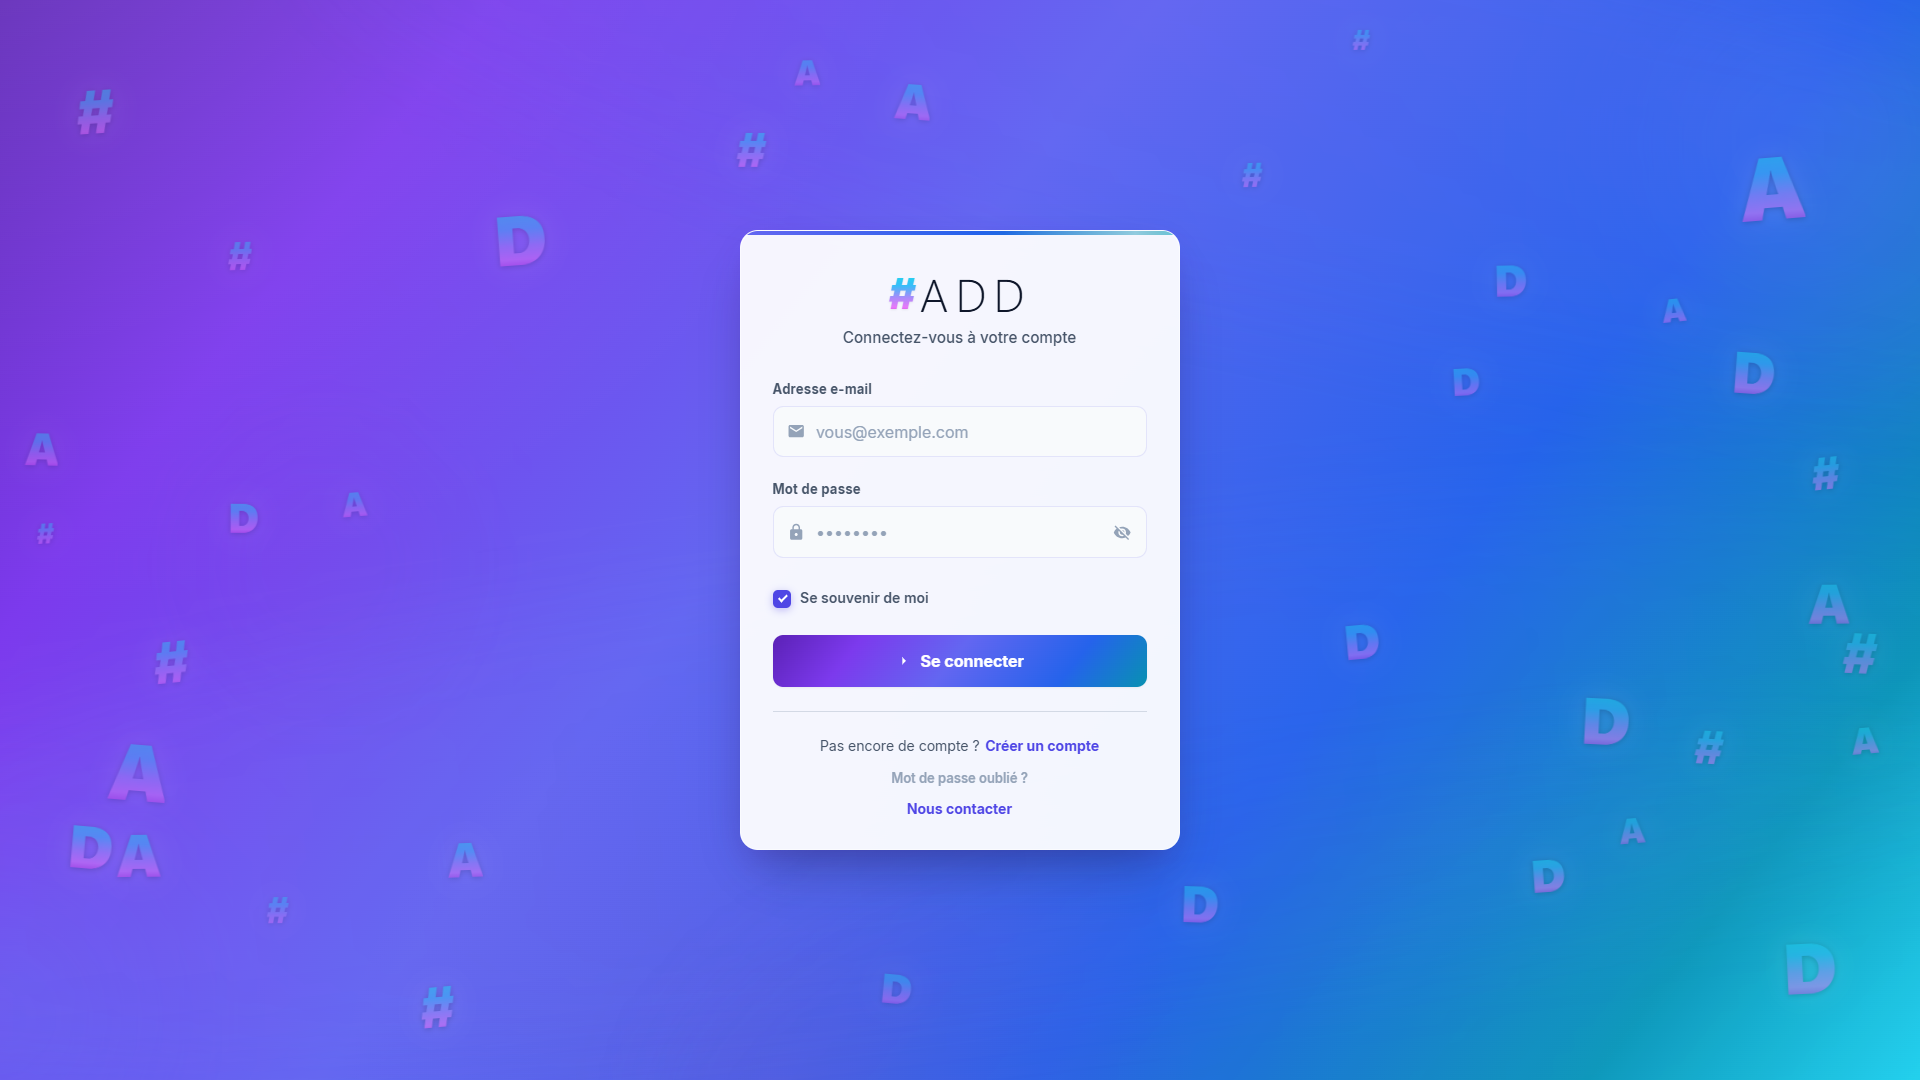
\includegraphics[width=0.9\textwidth]{auth-login.png}
\caption{Écran de connexion par adresse e-mail et mot de passe.}
\label{fig:auth-login}
\end{figure}

La figure~\ref{fig:auth-login} présente l'écran de connexion de la plateforme E-Services. Cette interface permet à l'utilisateur de saisir son adresse e-mail et son mot de passe afin d'accéder aux fonctionnalités correspondant à son rôle. Elle constitue le point d'entrée principal vers les espaces sécurisés de l'application et s'appuie sur le mécanisme d'authentification Laravel Sanctum décrit précédemment.

\subsubsection{Inscription}

\begin{figure}[H]
\centering
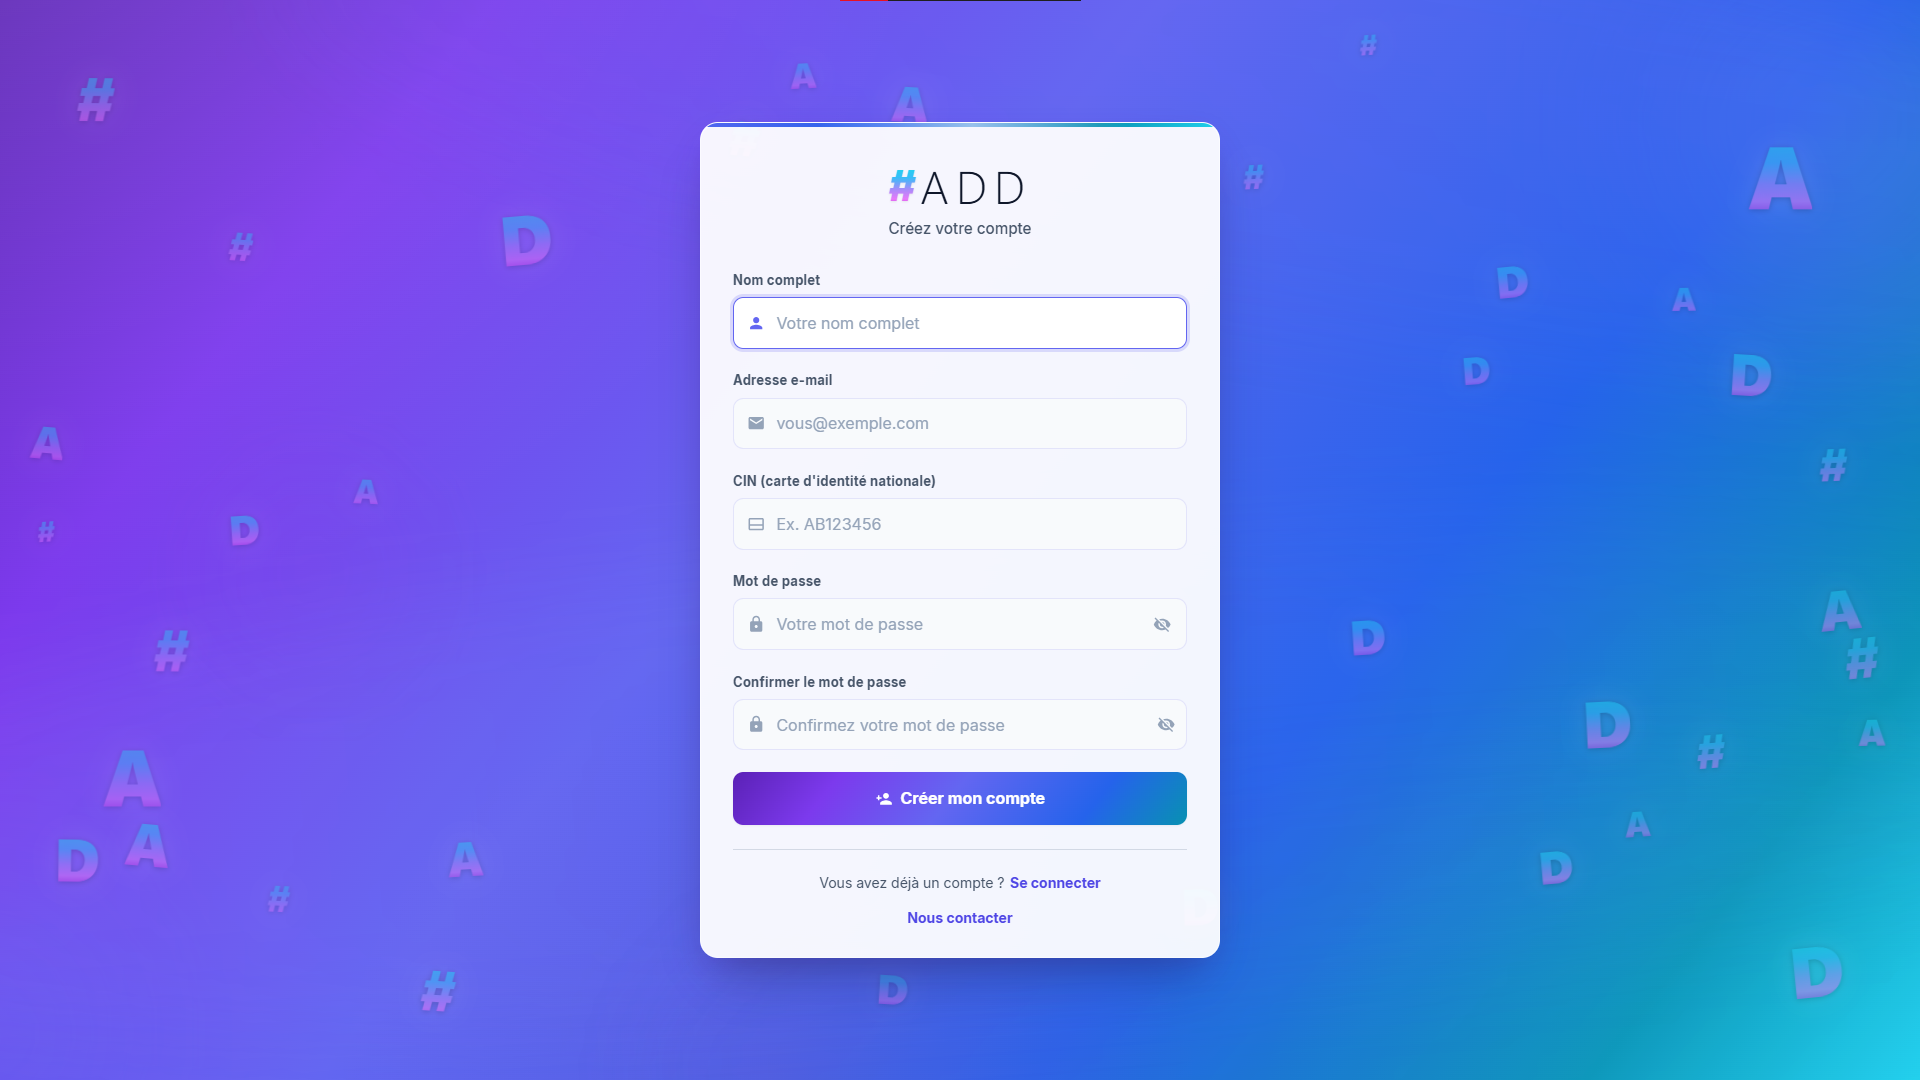
\includegraphics[width=0.9\textwidth]{auth-register.png}
\caption{Formulaire d'inscription d'un nouvel usager.}
\label{fig:auth-register}
\end{figure}

La figure~\ref{fig:auth-register} illustre le formulaire d'inscription destiné aux nouveaux usagers. Cette interface permet de collecter les informations nécessaires à la création d'un compte, notamment le nom complet, l'adresse e-mail, le CIN et le mot de passe. Les données saisies sont validées avant leur enregistrement afin de garantir leur cohérence et leur intégrité.

\newpage
\subsubsection{Récupération du mot de passe}

\begin{figure}[H]
\centering
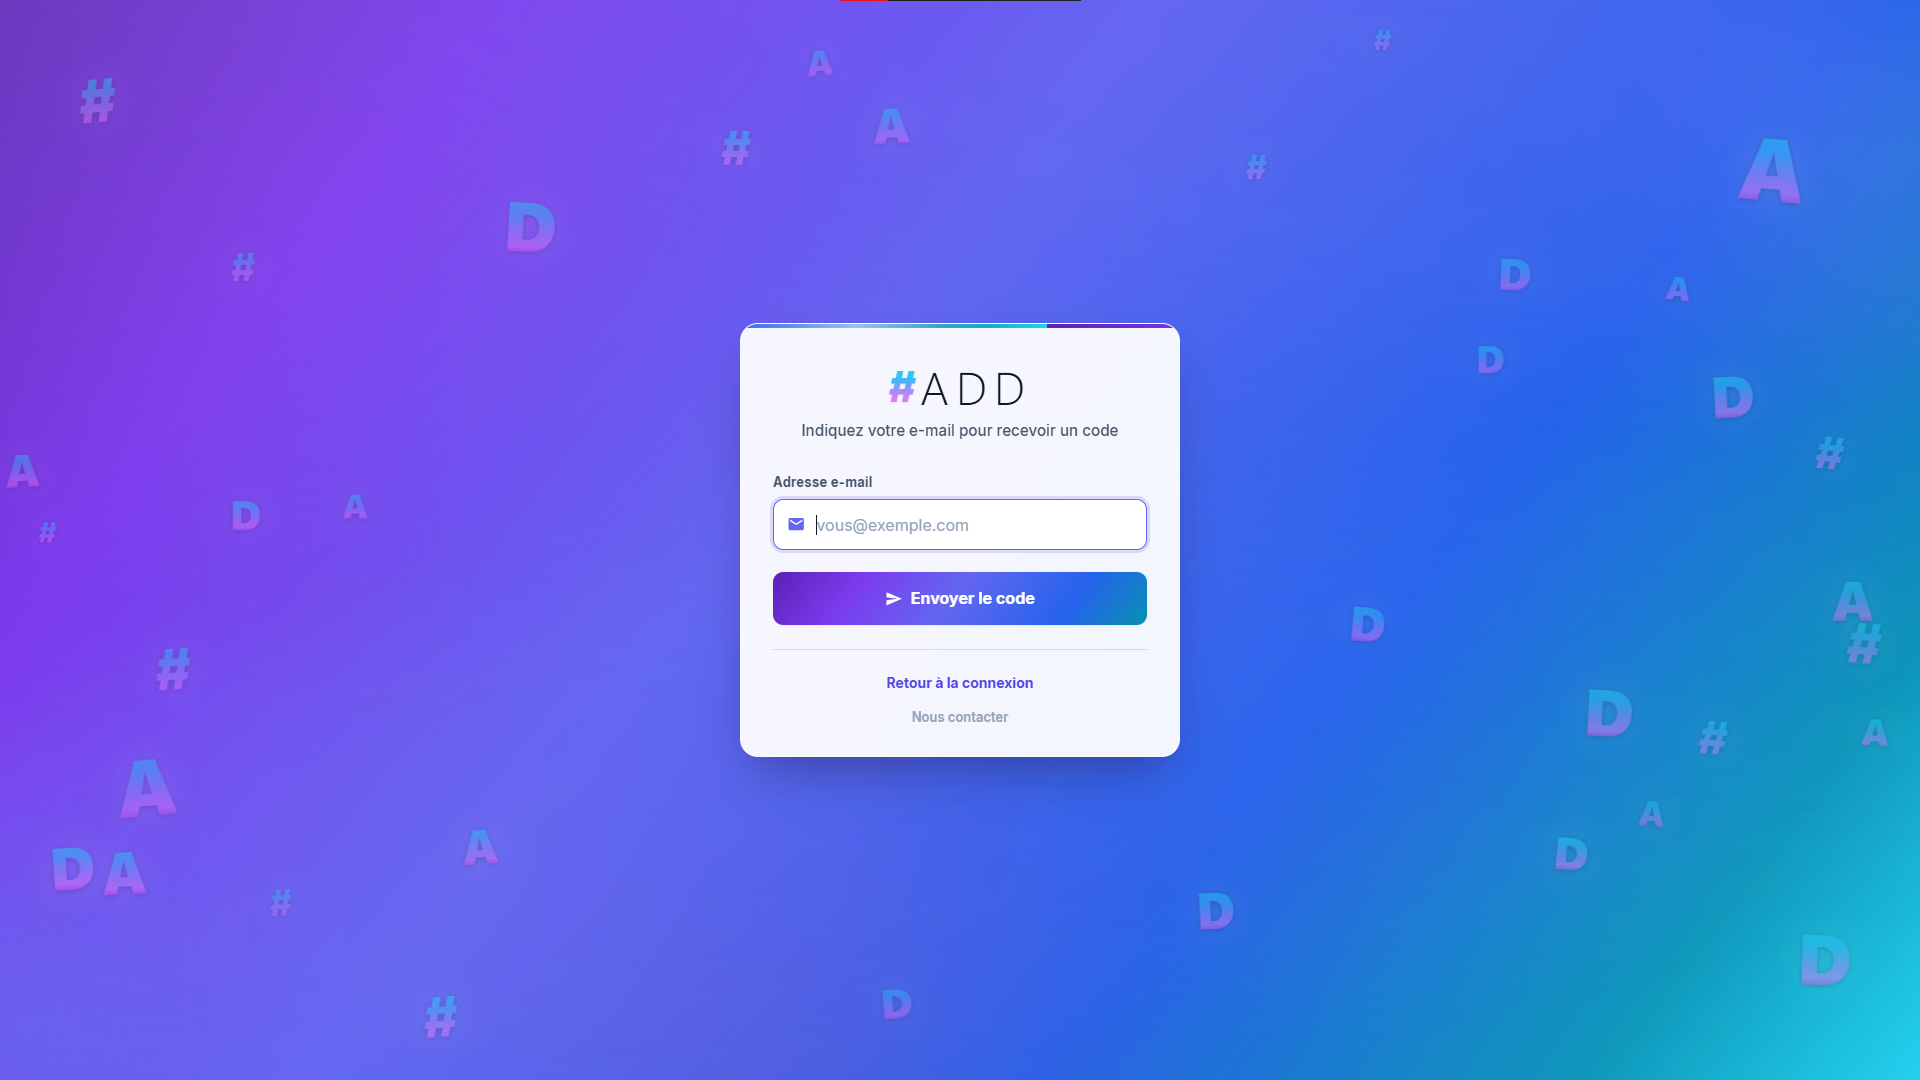
\includegraphics[width=0.9\textwidth]{auth-forgot-password.png}
\caption{Première étape de récupération du mot de passe oublié.}
\label{fig:auth-forgot-password}
\end{figure}

La figure~\ref{fig:auth-forgot-password} présente la première étape de récupération du mot de passe. L'utilisateur renseigne son adresse e-mail afin de recevoir un code de vérification. Cette fonctionnalité améliore l'autonomie de l'utilisateur tout en maintenant un niveau de sécurité adapté à la gestion des accès.
\newpage
\begin{figure}[H]
\centering
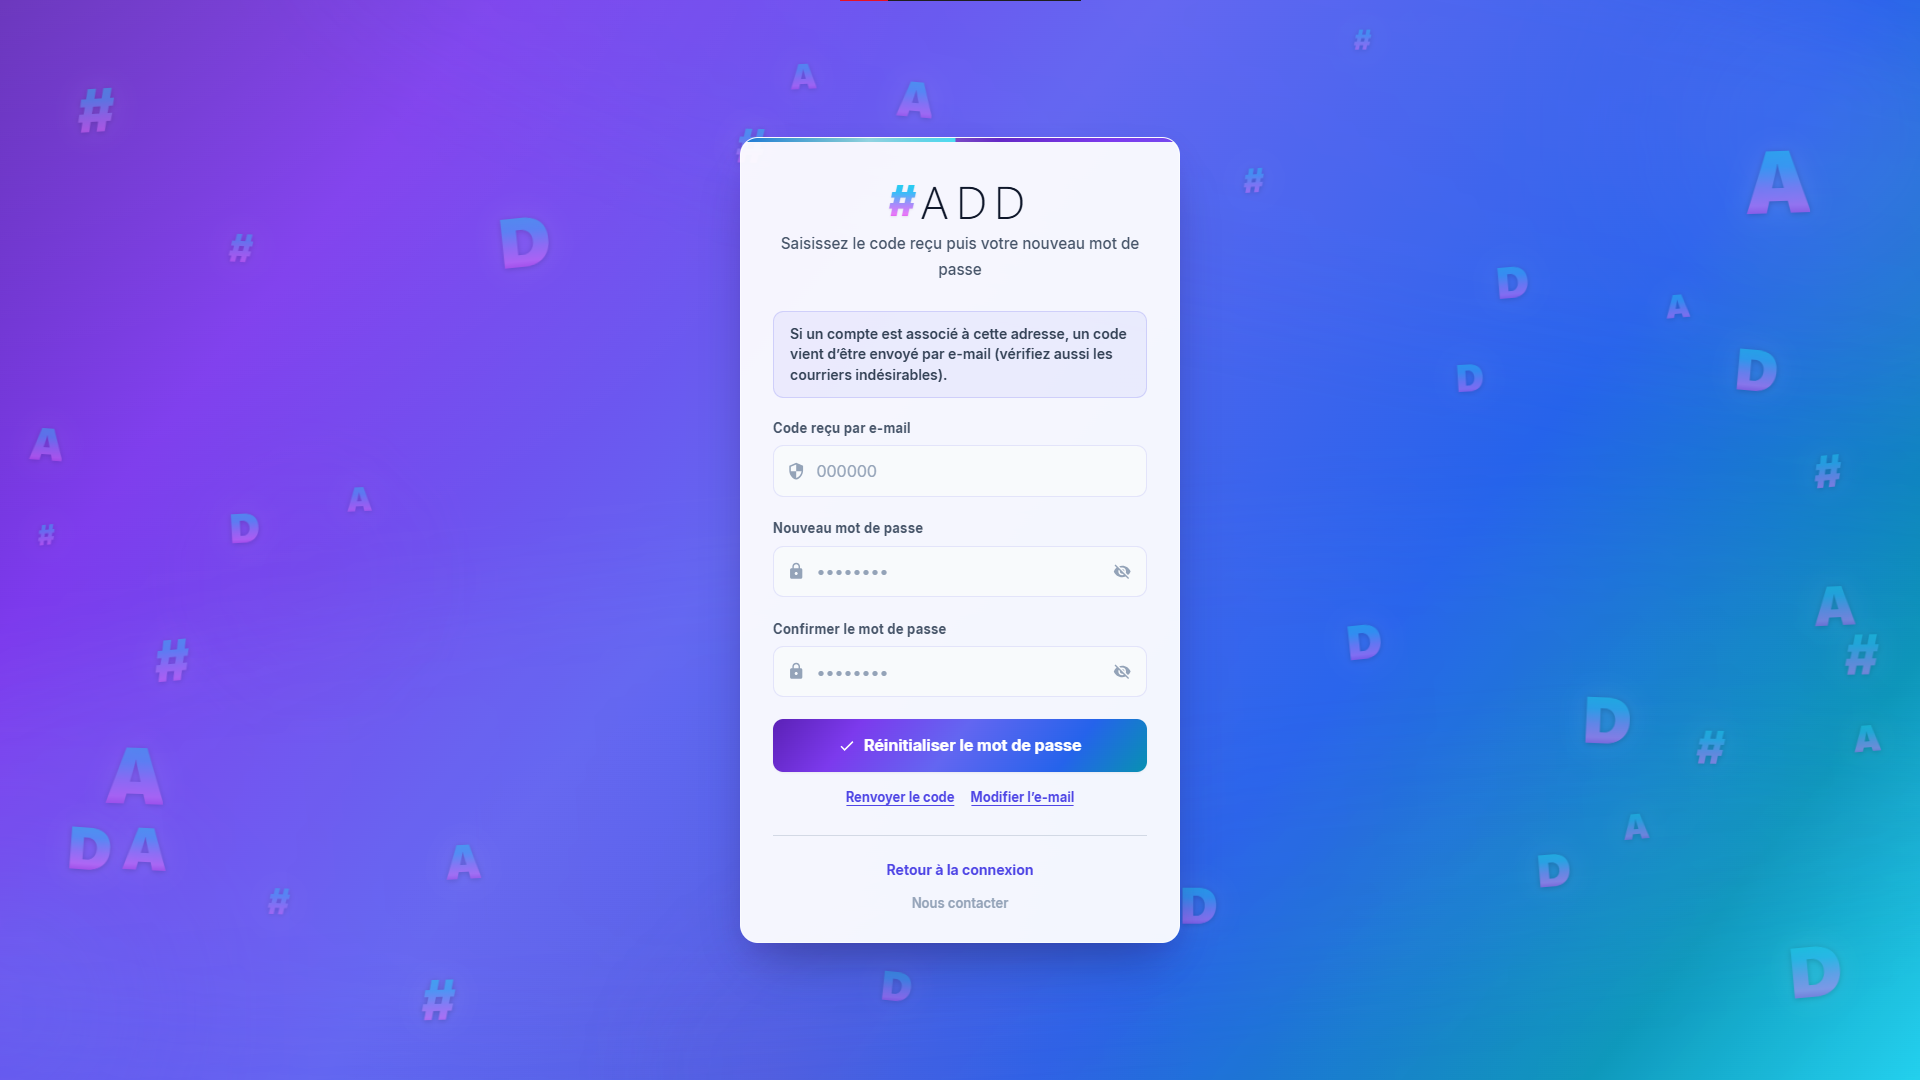
\includegraphics[width=0.9\textwidth]{auth-reset-password.png}
\caption{Seconde étape de réinitialisation du mot de passe.}
\label{fig:auth-reset-password}
\end{figure}

La figure~\ref{fig:auth-reset-password} montre la seconde étape du processus de réinitialisation. Après réception du code de vérification par e-mail, l'utilisateur peut définir un nouveau mot de passe. Le système vérifie la validité du code ainsi que la conformité des informations saisies avant la mise à jour des données d'authentification.

\newpage
\subsection{Interface générale du portail administrateur}

Le portail administrateur repose sur une interface structurée autour d'un menu latéral, d'un en-tête, d'une identité visuelle et d'un système de notifications. Ces éléments assurent une navigation claire entre les différents modules du back-office.

\subsubsection{Menu latéral}

\begin{figure}[H]
\centering
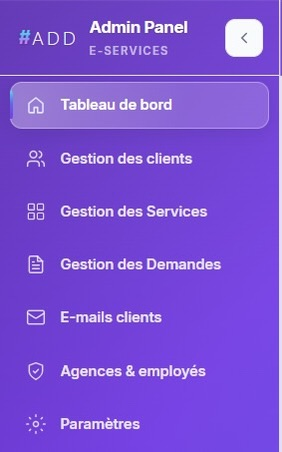
\includegraphics[width=0.45\textwidth]{admin-sidebar-expanded.jpeg}
\caption{Menu latéral du portail administrateur en mode développé.}
\label{fig:admin-sidebar-expanded}
\end{figure}

La figure~\ref{fig:admin-sidebar-expanded} présente le menu latéral du portail administrateur en mode développé. Il regroupe les principaux modules de gestion, notamment le tableau de bord, les clients, les services, les demandes, les e-mails, les agences, les employés et les paramètres.
\newpage
\subsubsection{En-tête et identité visuelle}

\begin{figure}[H]
\centering

\includegraphics[width=1\textwidth]{admin-header.png}
\caption{En-tête du portail administrateur avec titre, notifications et profil connecté.}
\label{fig:admin-header}
\end{figure}

La figure~\ref{fig:admin-header} présente l'en-tête du portail administrateur. Il affiche le titre de la page courante, l'accès aux notifications et un message d'accueil personnalisé indiquant l'utilisateur connecté.

\begin{figure}[H]
\centering

\includegraphics[width=1\textwidth]{admin-brand-mark.png}
\caption{Élément de marque \#ADD intégré dans l'en-tête.}
\label{fig:admin-brand-mark}
\end{figure}

La figure~\ref{fig:admin-brand-mark} met en évidence l'identité visuelle de la plateforme. L'intégration du logo \#ADD dans l'en-tête permet de renforcer la cohérence graphique de l'application et d'assurer une continuité visuelle entre les différents modules.

\newpage
\subsection{Tableau de bord administratif}

Le tableau de bord administratif constitue l'écran principal de supervision de la plateforme. Il offre à l'administrateur une vision globale sur les entités gérées, les demandes déposées et l'état général de l'activité.

\begin{figure}[H]
\centering
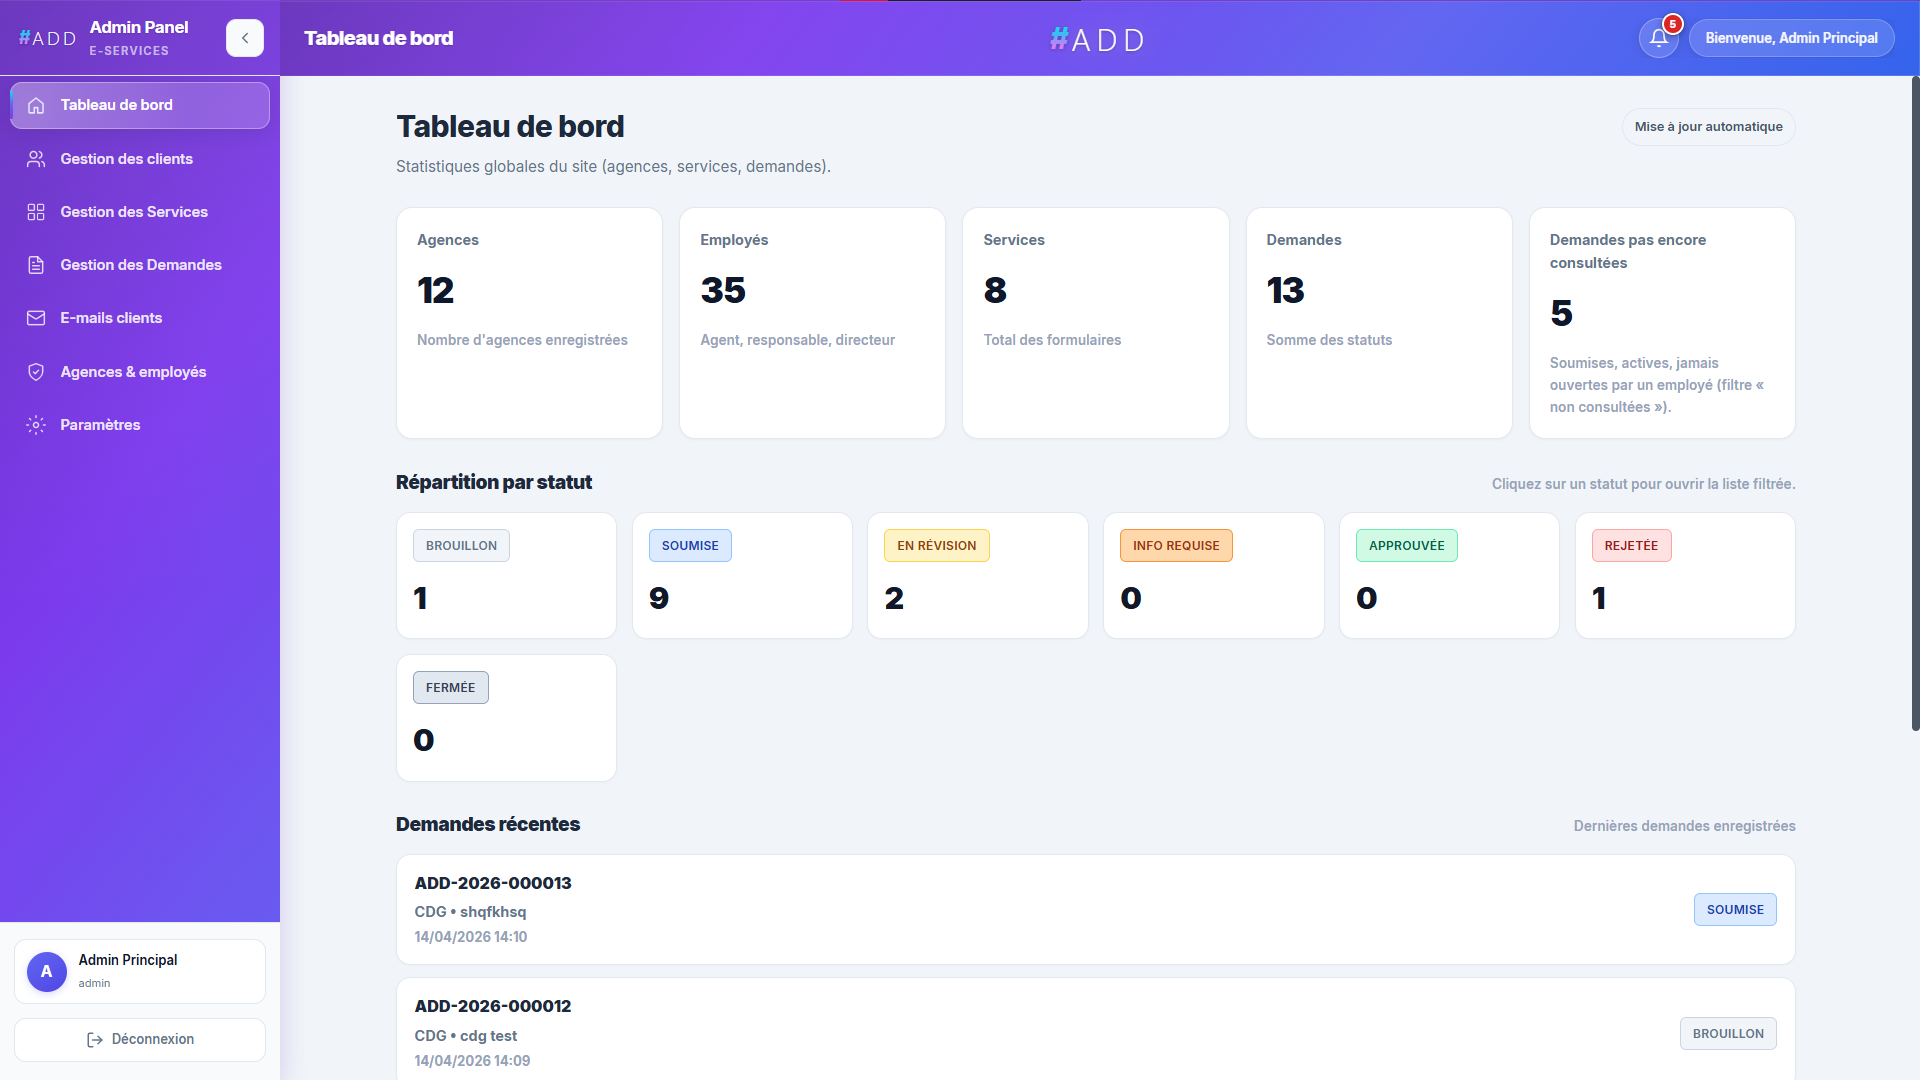
\includegraphics[width=0.95\textwidth]{admin-dashboard-top.png}
\caption{Tableau de bord administrateur avec indicateurs globaux et répartition des demandes par statut.}
\label{fig:admin-dashboard-top}
\end{figure}

La figure~\ref{fig:admin-dashboard-top} présente la partie supérieure du tableau de bord administrateur. Les cartes de synthèse affichent les principaux indicateurs du système, notamment le nombre d'agences, d'employés, de services, de demandes et de demandes non encore consultées. La répartition par statut permet de visualiser l'état d'avancement des dossiers selon le workflow implémenté.

\begin{figure}[H]
\centering
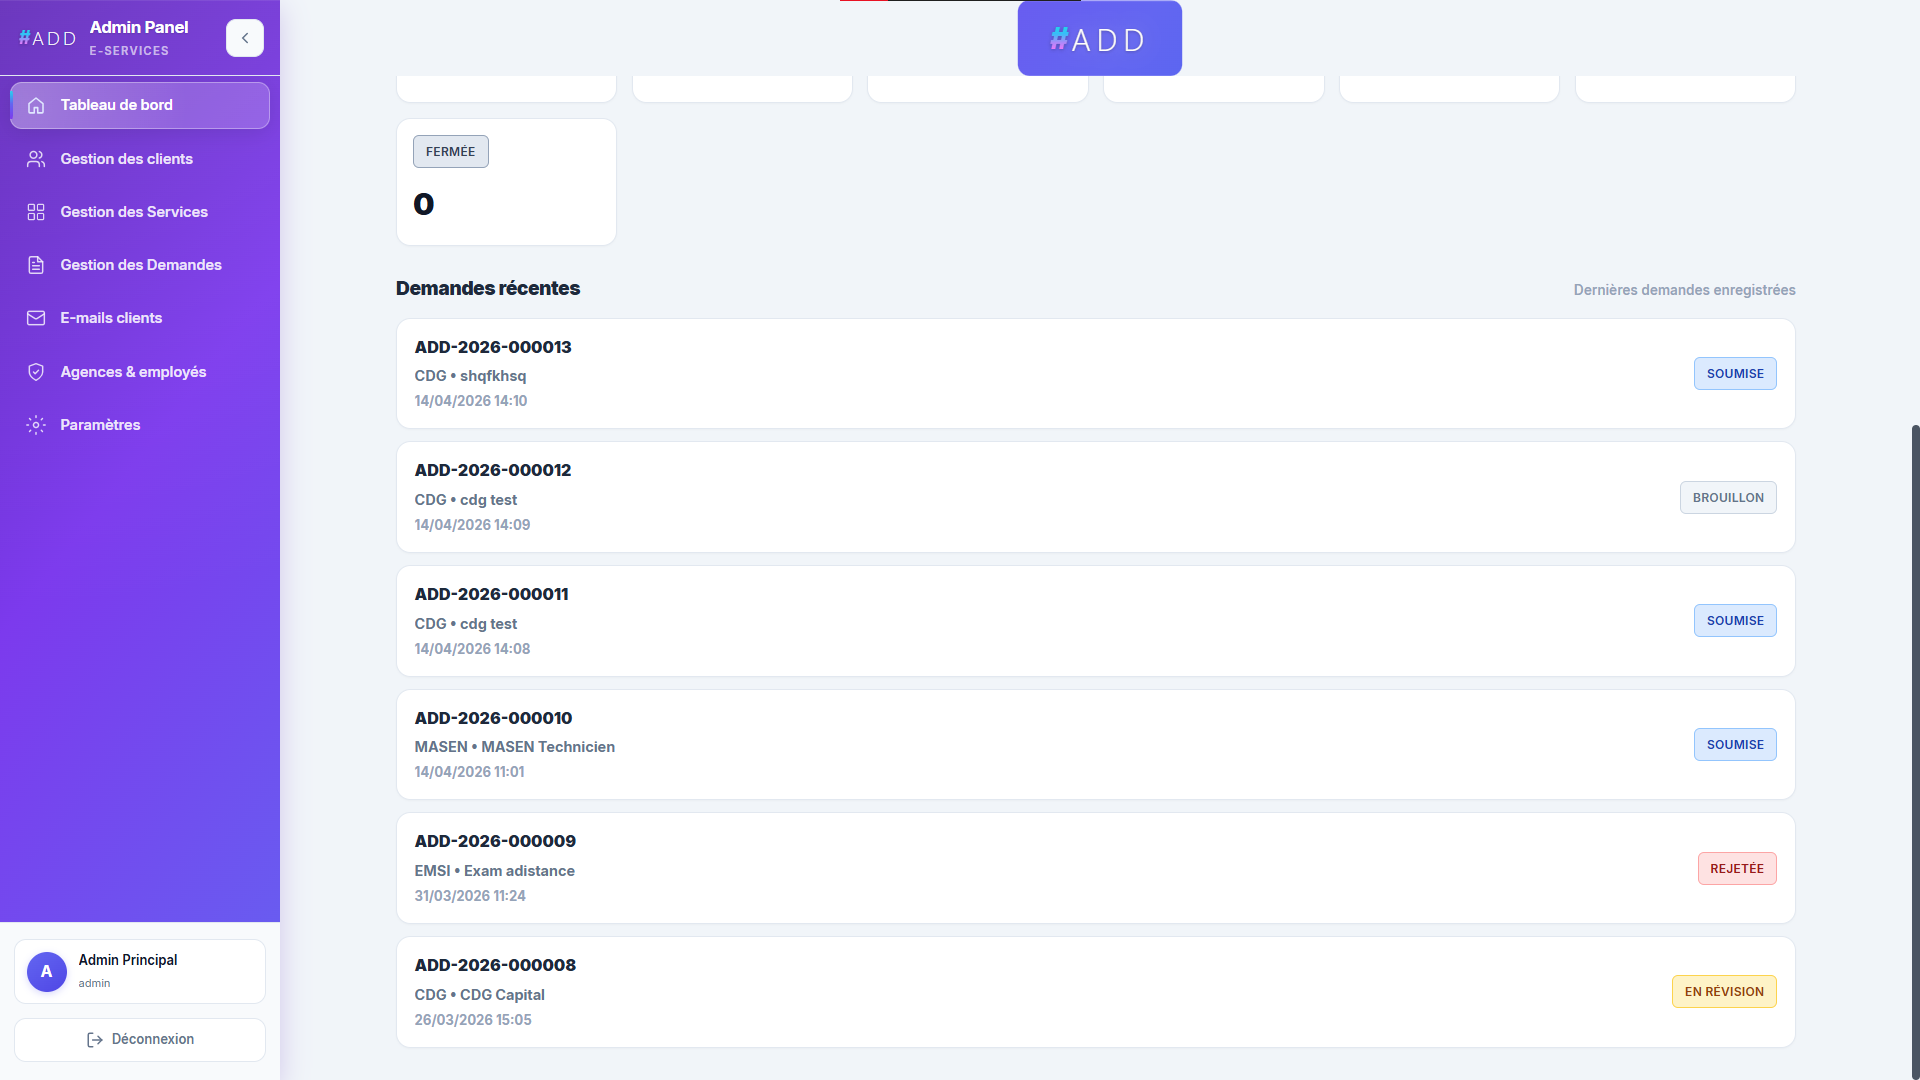
\includegraphics[width=0.95\textwidth]{admin-dashboard-buttom.png}
\caption{Liste des demandes récentes affichée dans le tableau de bord.}
\label{fig:admin-dashboard-buttom}
\end{figure}

La figure~\ref{fig:admin-dashboard-bottom} complète le tableau de bord en présentant les demandes les plus récentes. Chaque ligne affiche la référence métier, l'entité concernée, la date et l'état courant du dossier. Cette vue facilite le suivi quotidien de l'activité et permet d'identifier rapidement les demandes nécessitant une intervention.

\newpage
\subsection{Gestion des services}

Le module de gestion des services permet à l'administrateur de créer, modifier, consulter et organiser les services proposés par les agences. Il constitue un élément central de la plateforme, car il conditionne les formulaires disponibles pour les usagers.

\begin{figure}[H]
\centering
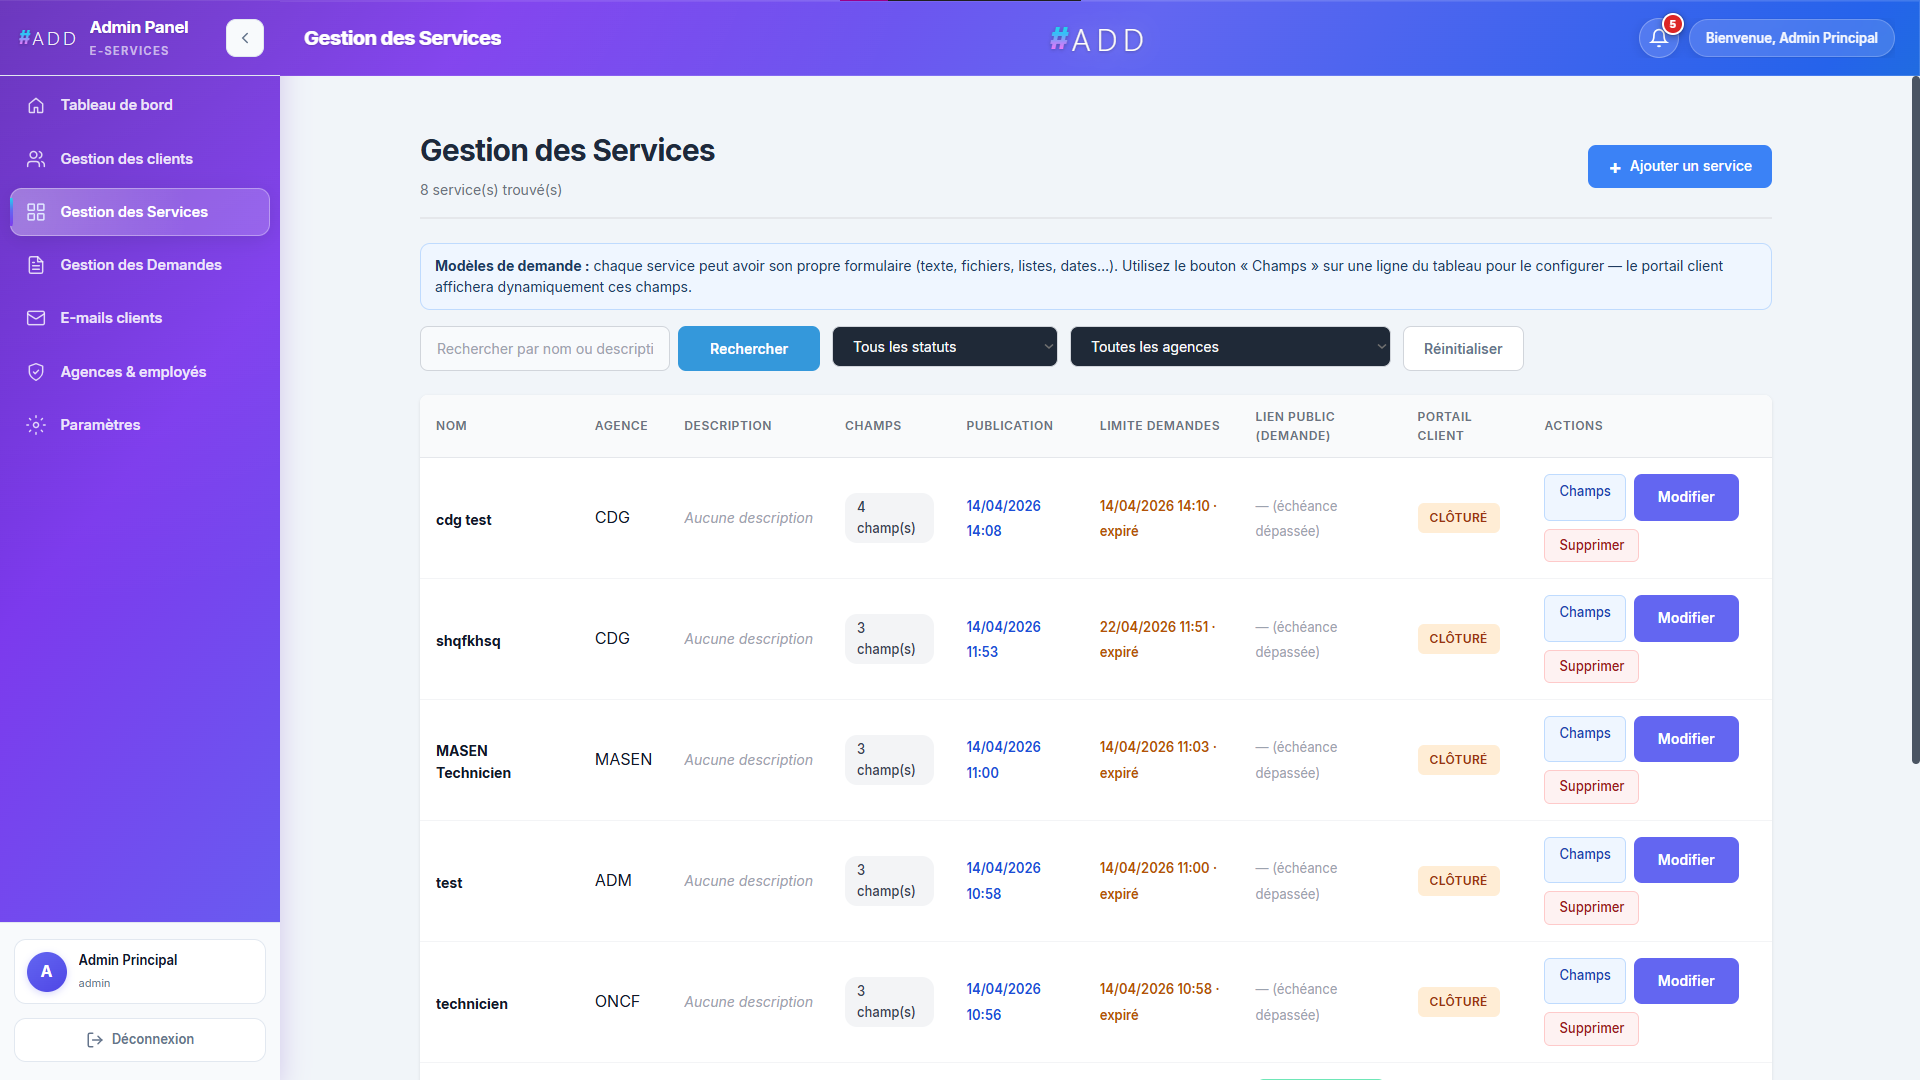
\includegraphics[width=0.95\textwidth]{admin-services-list.png}
\caption{Interface de consultation de la liste des services.}
\label{fig:admin-services-list}
\end{figure}

La figure~\ref{fig:admin-services-list} présente la liste des services disponibles dans la plateforme. Cette interface permet à l'administrateur de consulter les services existants, leurs informations principales et les actions de gestion associées.

\begin{figure}[H]
\centering
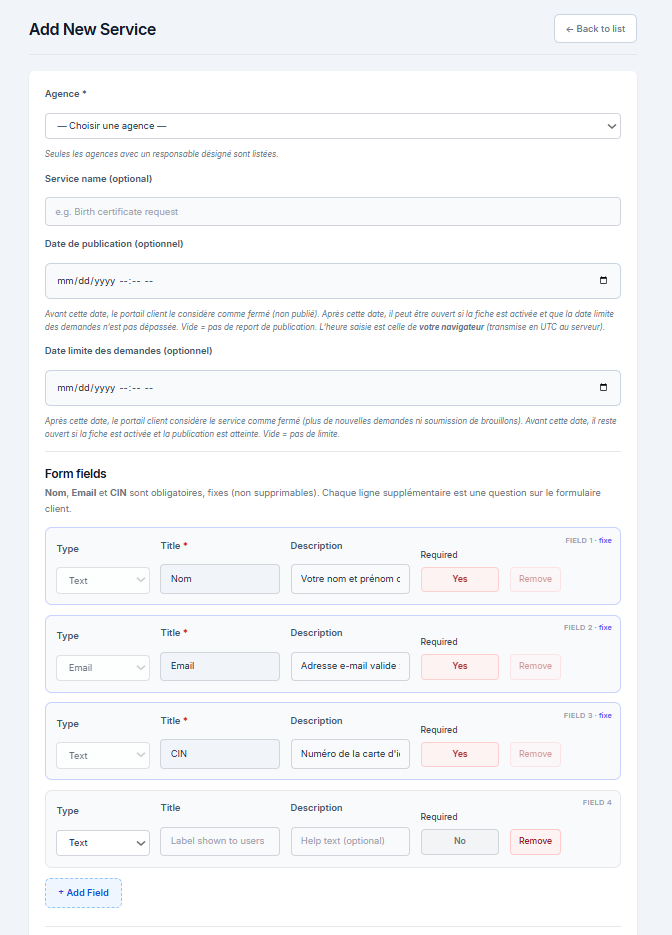
\includegraphics[width=0.95\textwidth]{admin-service-add.png}
\caption{Interface d'ajout d'un nouveau service.}
\label{fig:admin-service-add}
\end{figure}

La figure~\ref{fig:admin-service-add} illustre le formulaire d'ajout d'un nouveau service. Cette interface permet de renseigner les informations nécessaires à la publication du service et à la configuration de ses champs dynamiques.

\newpage
\subsection{Gestion des demandes}

Le module de gestion des demandes permet le suivi, l'affectation et le changement d'état des dossiers déposés par les usagers. Il assure la traçabilité du traitement et facilite la coordination entre les différents profils du back-office.

\begin{figure}[H]
\centering
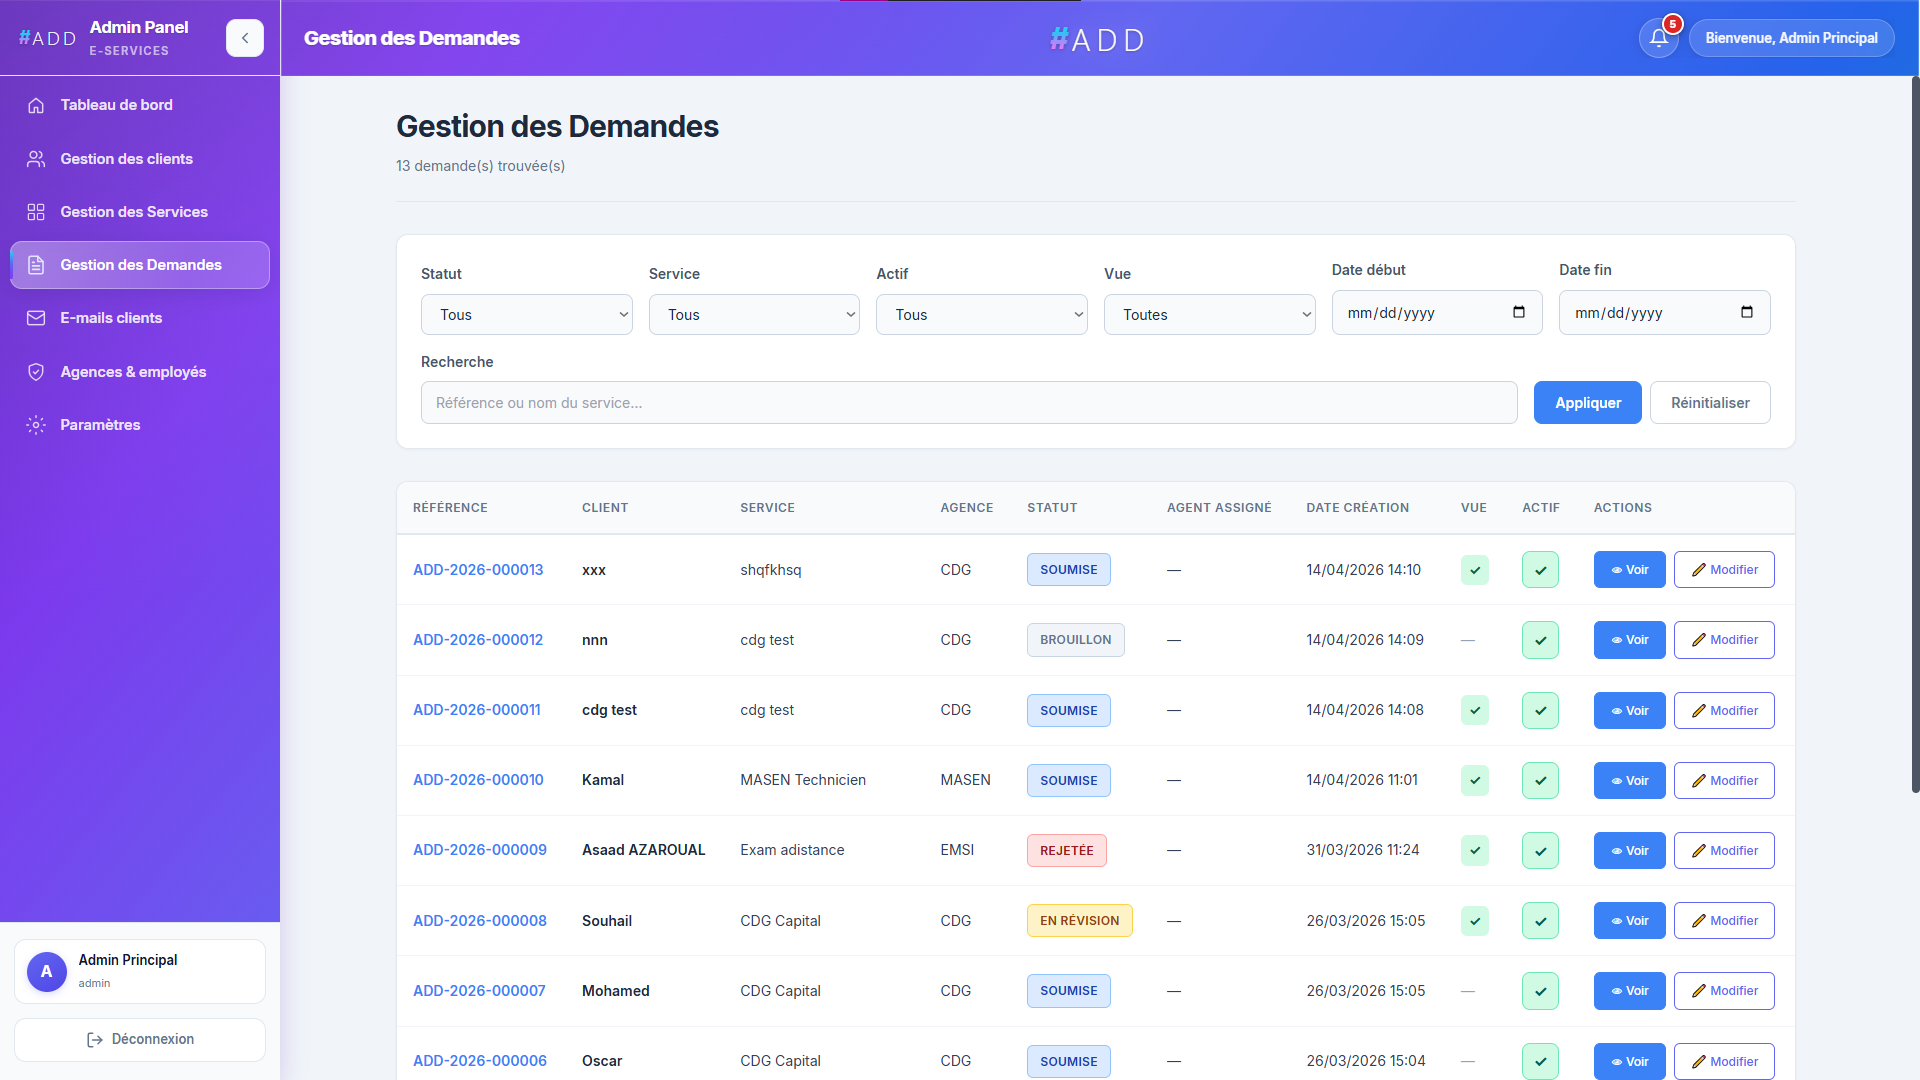
\includegraphics[width=0.95\textwidth]{admin-requests-list.png}
\caption{Interface de gestion et de suivi des demandes déposées.}
\label{fig:admin-requests-list}
\end{figure}

La figure~\ref{fig:admin-requests-list} présente la liste des demandes enregistrées dans le système. Elle permet de consulter les informations principales de chaque dossier, telles que la référence, le demandeur, le service concerné, la date et l'état de traitement.

\newpage
\subsection{Gestion des clients}

Le module de gestion des clients permet à l'administrateur de consulter les comptes clients et d'ajouter de nouveaux usagers à la plateforme.

\begin{figure}[H]
\centering
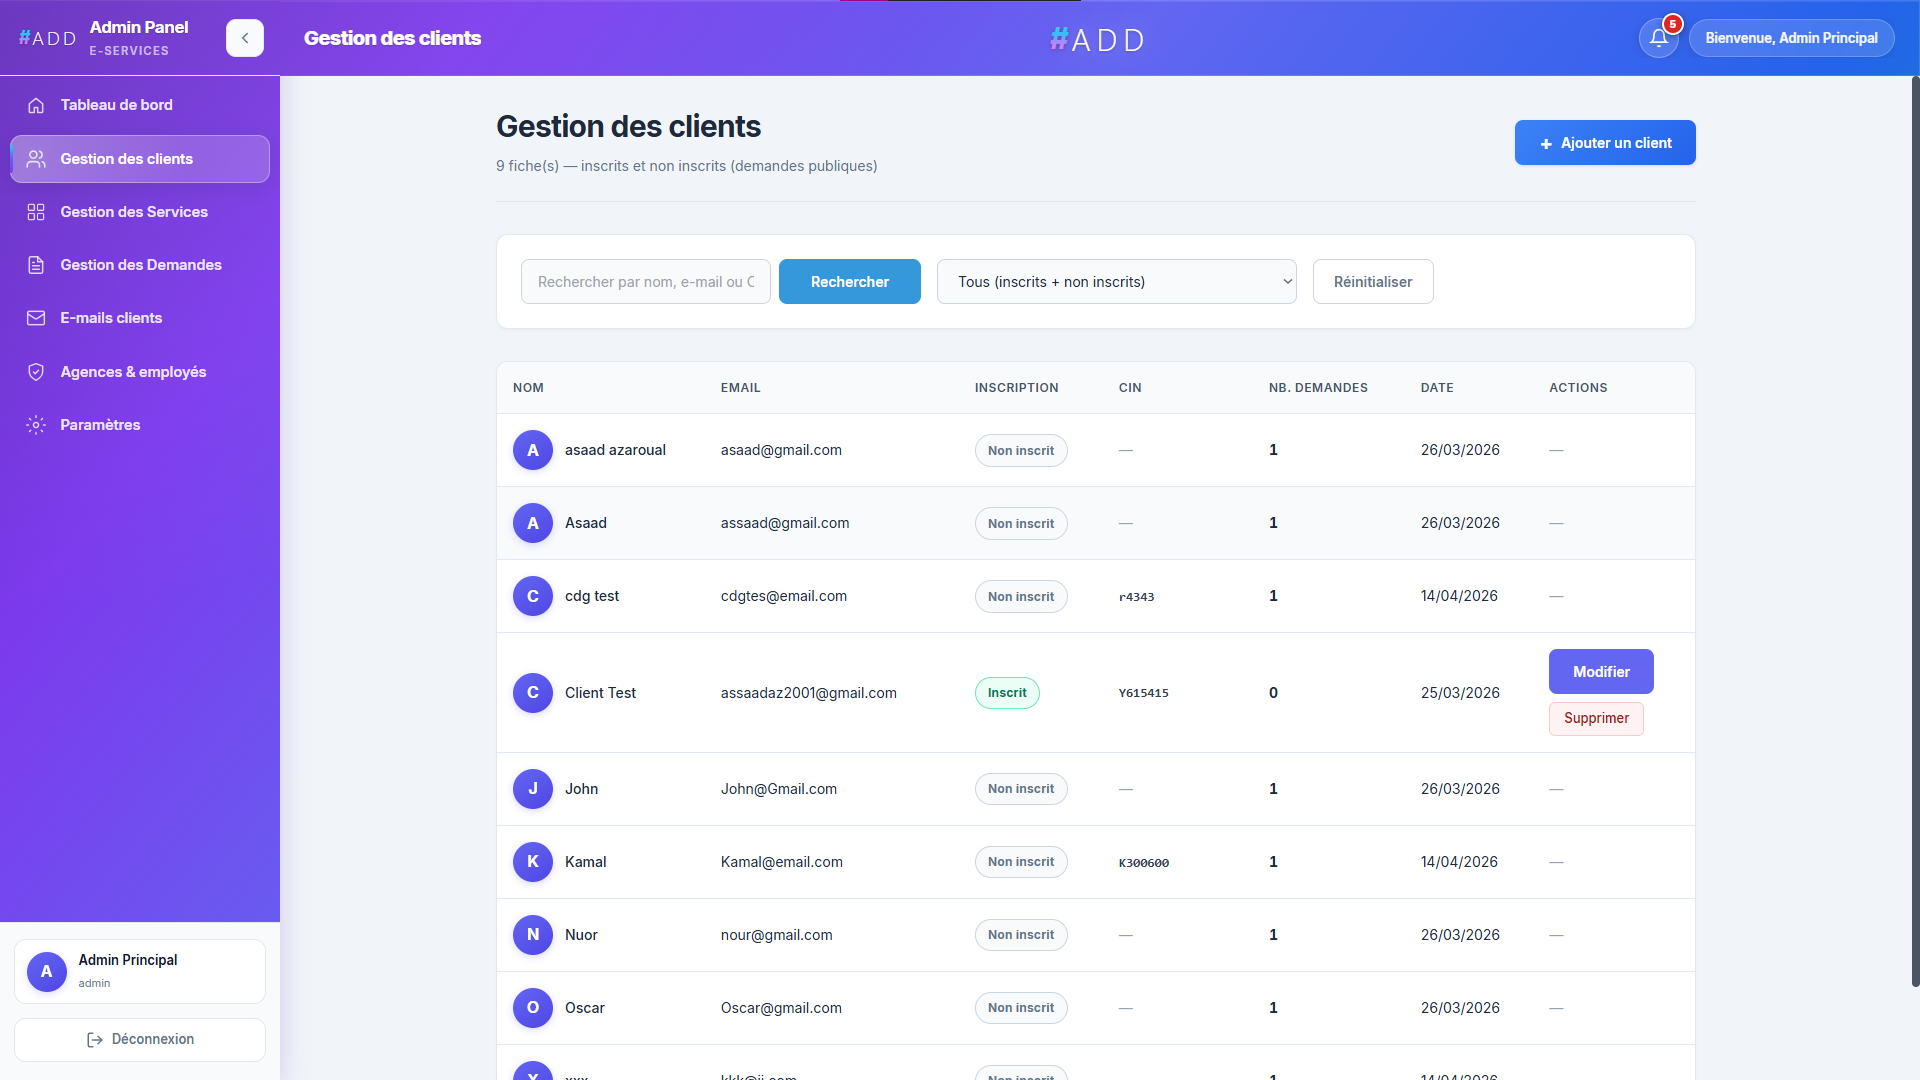
\includegraphics[width=0.95\textwidth]{admin-clients-list.png}
\caption{Interface de consultation de la liste des clients.}
\label{fig:admin-clients-list}
\end{figure}

La figure~\ref{fig:admin-clients-list} présente la liste des clients inscrits sur la plateforme. Cette interface facilite le suivi des comptes utilisateurs et permet à l'administrateur d'accéder rapidement aux informations essentielles relatives aux usagers.

\begin{figure}[H]
\centering
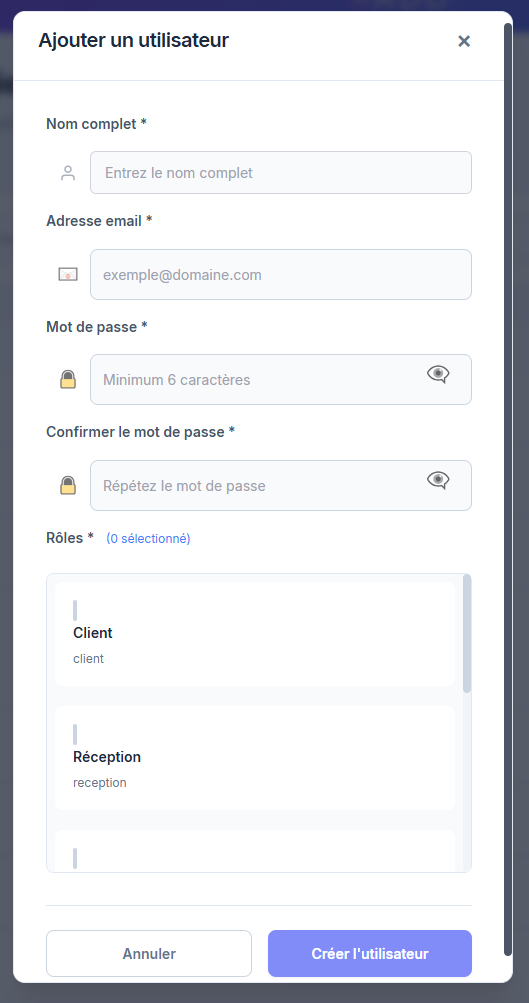
\includegraphics[width=0.7\textwidth]{admin-client-add.png}
\caption{Interface d'ajout d'un nouveau client.}
\label{fig:admin-client-add}
\end{figure}

La figure~\ref{fig:admin-client-add} illustre le formulaire d'ajout d'un nouveau client. L'administrateur peut y saisir les informations nécessaires à la création du compte utilisateur, ce qui permet d'assurer une gestion centralisée des usagers.

\newpage
\subsection{Gestion des agences}

Le module de gestion des agences permet d'administrer les entités institutionnelles participant à la plateforme. Chaque agence peut être associée à des services et à des employés.

\begin{figure}[H]
\centering
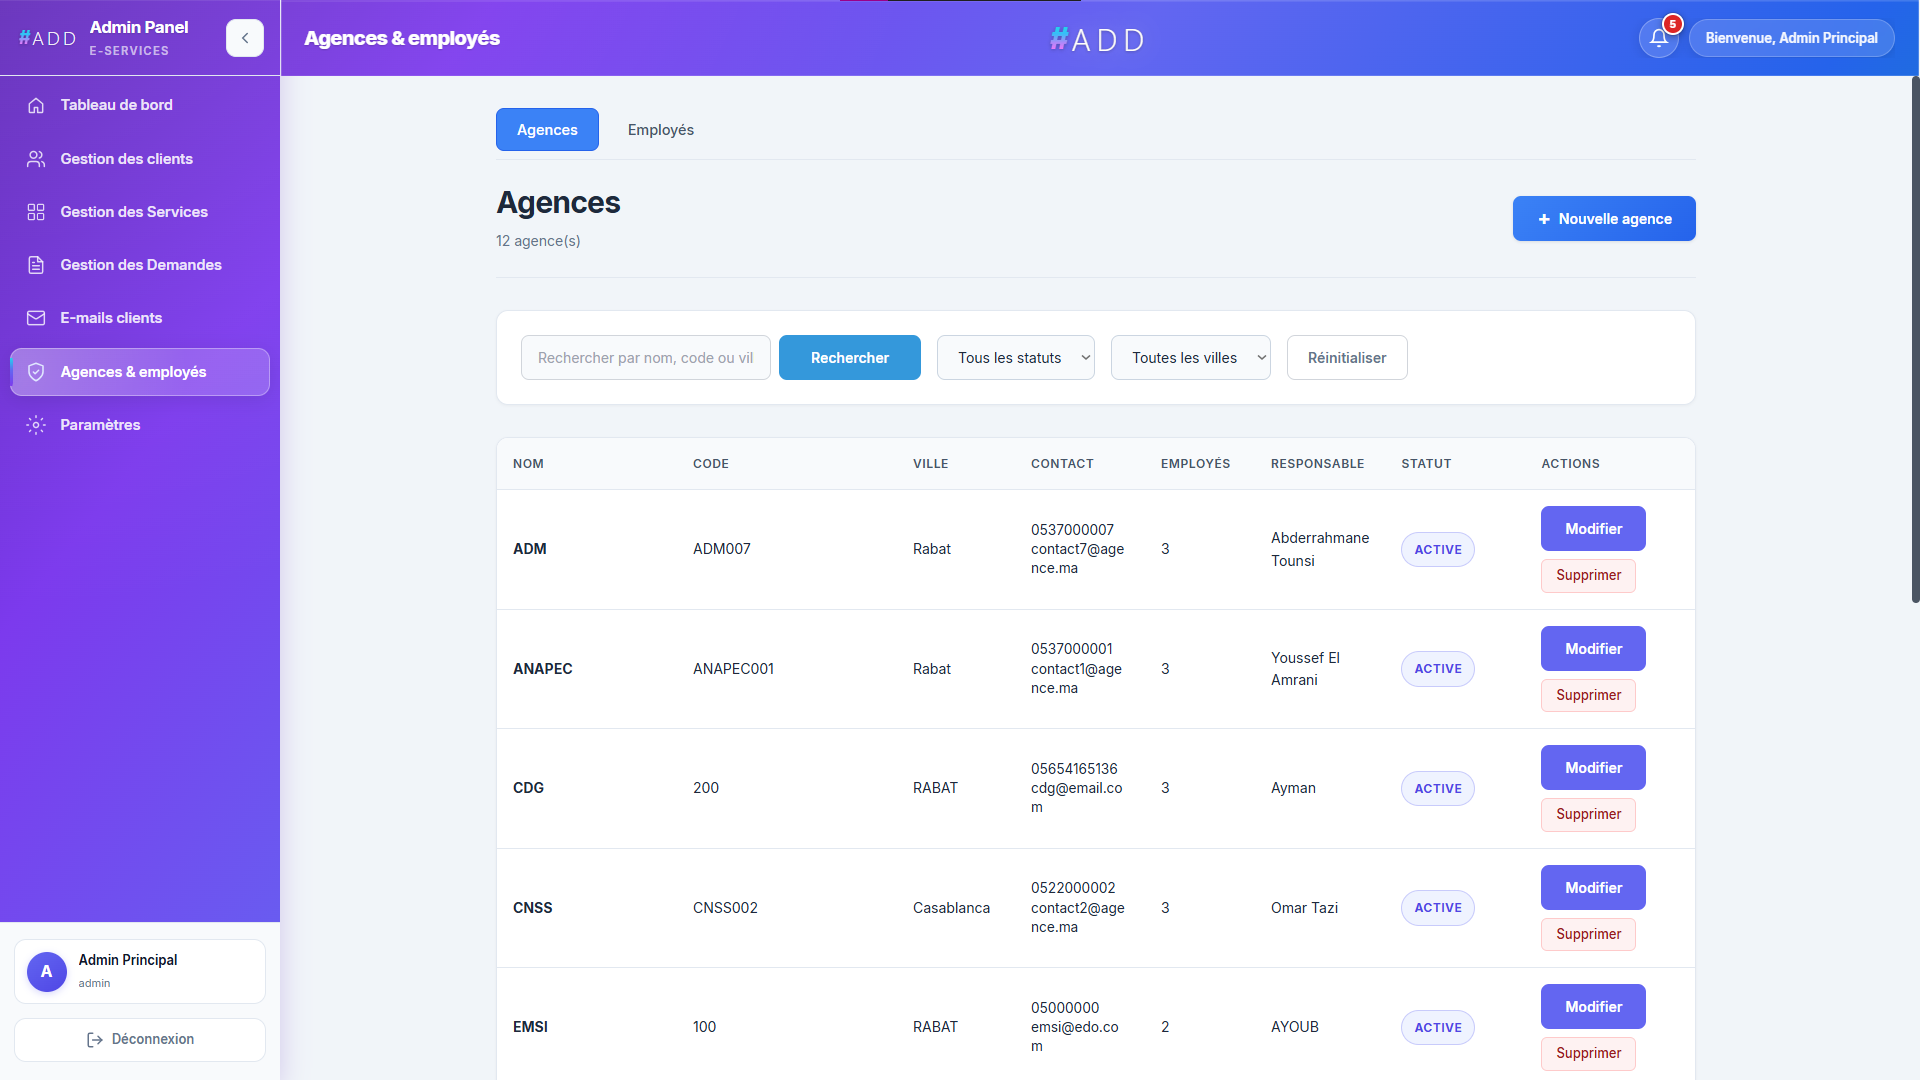
\includegraphics[width=0.95\textwidth]{admin-agencies-list.png}
\caption{Interface de consultation de la liste des agences.}
\label{fig:admin-agencies-list}
\end{figure}

La figure~\ref{fig:admin-agencies-list} présente la liste des agences enregistrées dans le système. Cette interface permet de consulter les informations principales de chaque agence et d'accéder aux actions de modification ou de gestion.

\begin{figure}[H]
\centering
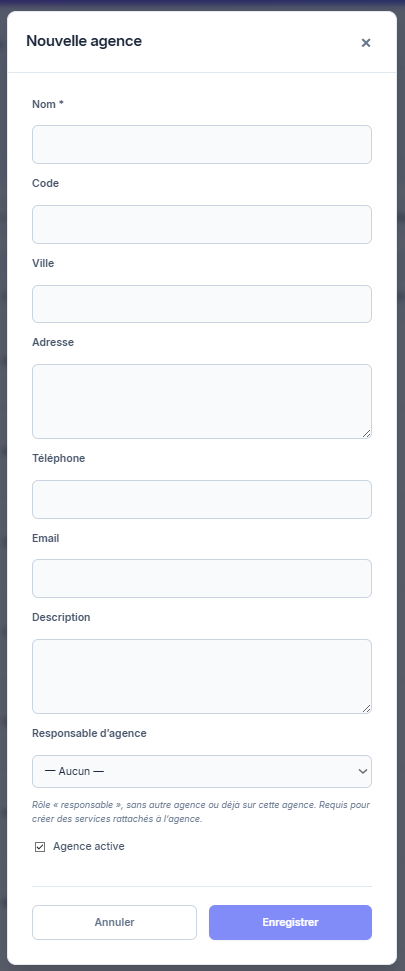
\includegraphics[width=0.5\textwidth]{admin-agency-add.png}
\caption{Interface d'ajout d'une nouvelle agence.}
\label{fig:admin-agency-add}
\end{figure}

La figure~\ref{fig:admin-agency-add} illustre le formulaire d'ajout d'une nouvelle agence. Cette fonctionnalité permet à l'administrateur d'enregistrer une nouvelle entité avec ses informations principales, afin de l'intégrer au processus de gestion des services et des demandes.

\newpage
\subsection{Gestion des employés}

Le module de gestion des employés permet d'administrer les comptes internes de la plateforme, notamment les agents, responsables et autres profils opérationnels. Chaque employé peut être associé à une agence et disposer d'un rôle adapté à ses responsabilités.

\begin{figure}[H]
\centering
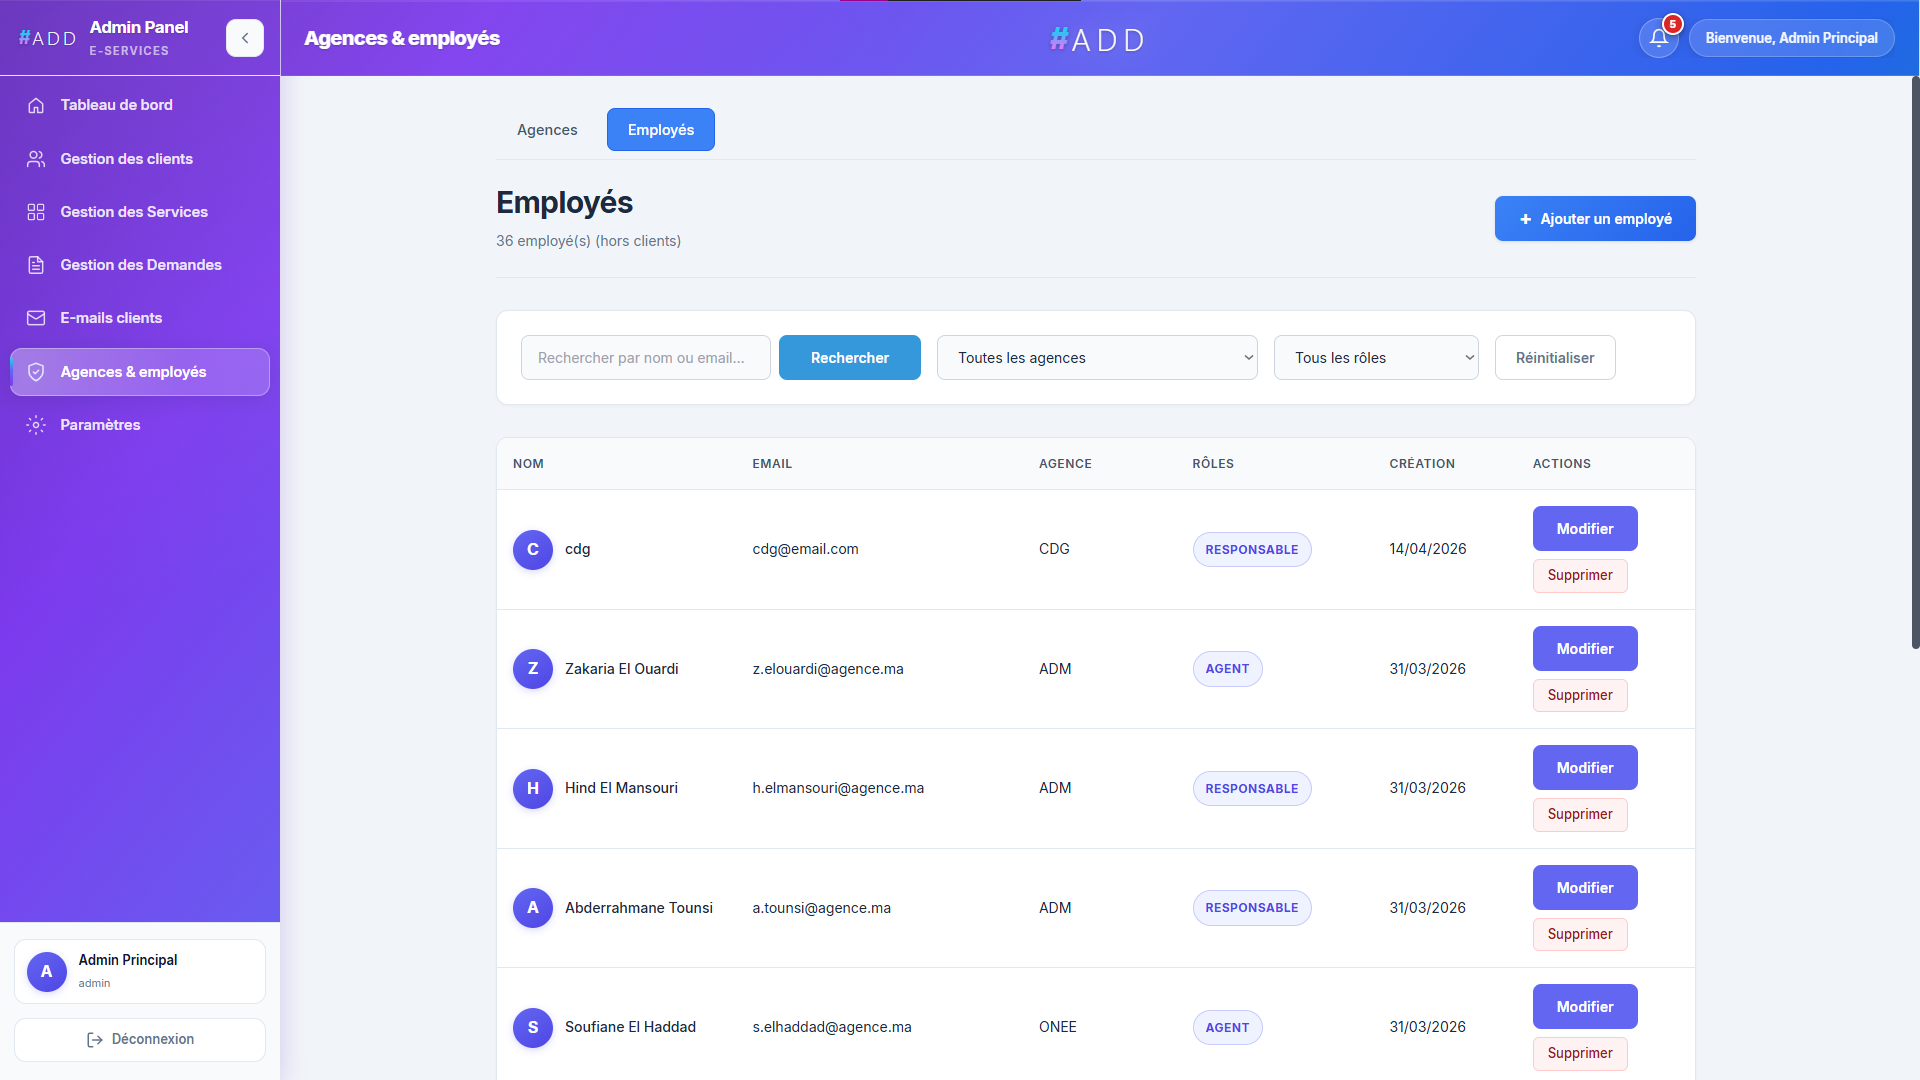
\includegraphics[width=0.95\textwidth]{admin-employees-list.png}
\caption{Interface de consultation de la liste des employés.}
\label{fig:admin-employees-list}
\end{figure}

La figure~\ref{fig:admin-employees-list} présente la liste des employés enregistrés dans le back-office. Cette interface facilite le suivi des comptes internes, de leurs rôles et de leur rattachement aux agences.

\begin{figure}[H]
\centering
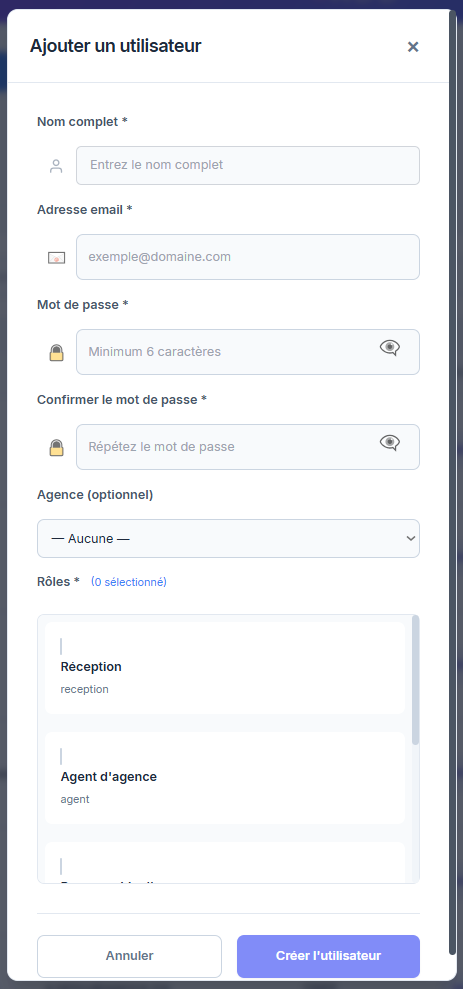
\includegraphics[width=0.6\textwidth]{admin-employee-add.png}
\caption{Interface d'ajout d'un nouvel employé.}
\label{fig:admin-employee-add}
\end{figure}

La figure~\ref{fig:admin-employee-add} illustre le formulaire d'ajout d'un nouvel employé. L'administrateur peut renseigner les informations personnelles, le rôle et l'agence de rattachement afin de créer un compte opérationnel conforme à l'organisation interne.

\newpage
\subsection{E-mails clients}

Le module des e-mails clients permet d'assurer la communication avec les usagers depuis le back-office. Il complète le système de notifications automatiques en offrant une interface dédiée aux échanges administratifs.

\begin{figure}[H]
\centering
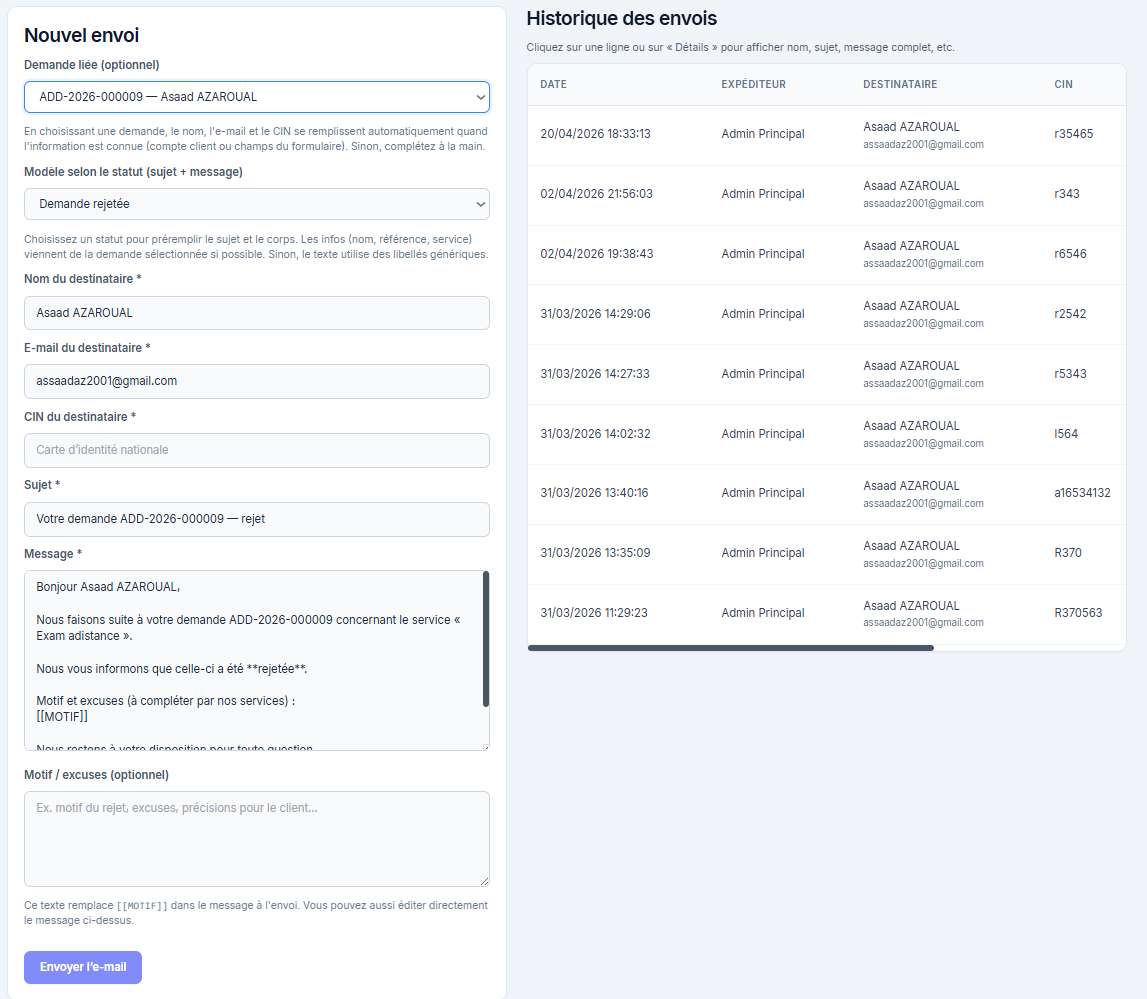
\includegraphics[width=1\textwidth]{admin-client-emails.png}
\caption{Interface de gestion des e-mails clients.}
\label{fig:admin-client-emails}
\end{figure}

La figure~\ref{fig:admin-client-emails} présente l'interface dédiée aux e-mails clients. Elle permet de centraliser les échanges avec les usagers et d'améliorer le suivi des communications liées aux demandes.

\newpage
\subsection{Notifications internes}

Les notifications internes permettent d'améliorer la réactivité des utilisateurs du back-office face aux nouvelles demandes soumises. Elles complètent les notifications envoyées par e-mail en offrant une alerte visuelle directement intégrée à l'interface.

\begin{figure}[H]
\centering

\includegraphics[width=0.15\textwidth]{notification-badge.png}
\caption{Badge de notification indiquant les demandes soumises non encore consultées.}
\label{fig:notification-badge}
\end{figure}

La figure~\ref{fig:notification-badge} montre le badge de notification intégré à l'en-tête du portail administratif. Le compteur indique le nombre de demandes soumises qui n'ont pas encore été consultées par un membre du personnel.

\begin{figure}[H]
\centering
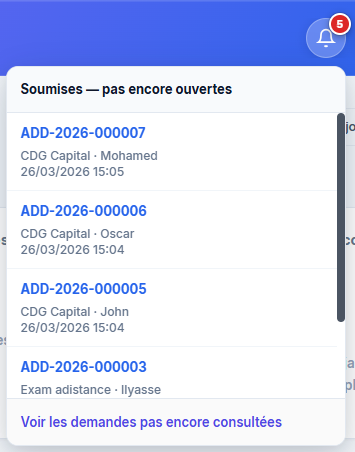
\includegraphics[width=0.4\textwidth]{notification-panel.png}
\caption{Panneau déroulant des notifications de demandes.}
\label{fig:notification-panel}
\end{figure}

La figure~\ref{fig:notification-panel} présente le panneau déroulant associé à l'icône de notification. Chaque entrée affiche les informations essentielles d'une demande, notamment sa référence, l'agence concernée, le demandeur et la date de soumission. Ce composant permet à l'administrateur ou à l'agent d'accéder rapidement aux nouvelles demandes sans quitter son contexte de travail.

\subsection{Paramètres utilisateur}

Le module des paramètres permet à l'utilisateur connecté de consulter et de modifier les informations liées à son profil. Cette fonctionnalité contribue à la personnalisation du compte et à la maintenance des données utilisateur.

\begin{figure}[H]
\centering
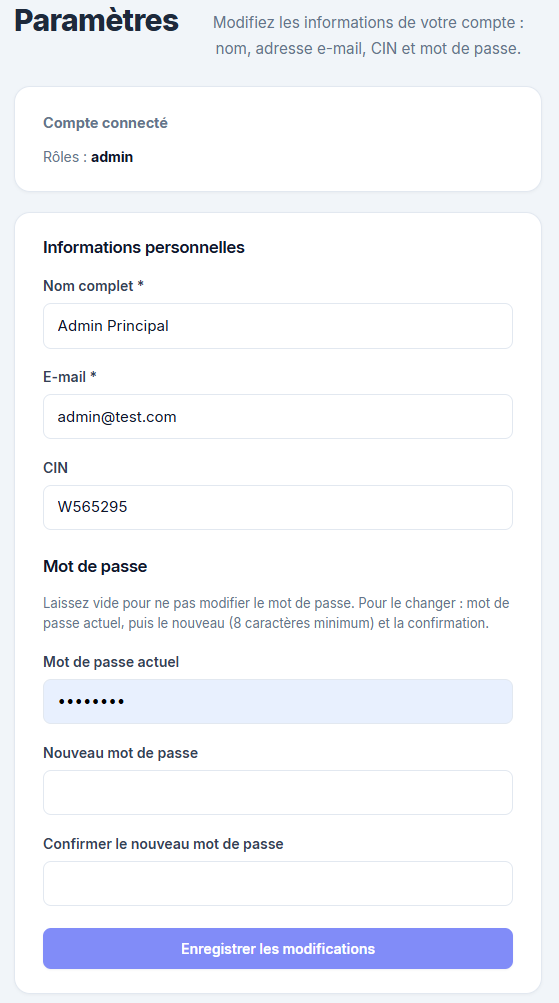
\includegraphics[width=0.6\textwidth]{admin-settings.png}
\caption{Interface de paramétrage du profil utilisateur.}
\label{fig:admin-settings}
\end{figure}

La figure~\ref{fig:admin-settings} présente l'écran des paramètres utilisateur. Cette interface permet la mise à jour des informations personnelles et contribue à la gestion autonome du profil.
```


\section{Interopérabilité et formats}

Les réponses d'erreur Laravel sont normalisées en JSON (messages de validation, codes HTTP). Les dates sont sérialisées en ISO-8601 côté API. La référence métier \texttt{ADD-AAAA-NNNNNN} est générée côté serveur pour les demandes \cite{owasp2021}.

\section{Journalisation et observabilité}

Laravel journalise via le canal configuré (\texttt{storage/logs/laravel.log} en développement). Les services métiers critiques (notifications) journalisent les succès et échecs d'envoi pour faciliter le diagnostic.

\section{Gestion des erreurs et robustesse}

Les contrôleurs s'appuient sur les exceptions HTTP de Laravel et sur les réponses structurées des Form Requests. Les transitions d'état vérifient le graphe autorisé avant persistance.

\section{Conclusion du chapitre}

L'implémentation décrite correspond au dépôt réalisé durant le stage : une API Laravel authentifiée par session Sanctum, un frontend React/Vite, une base PostgreSQL structurée par migrations, et des modules métiers (services dynamiques, demandes, agences, notifications). Le chapitre suivant présente les tests et la validation \cite{ieee1012,sommerville2016}.

\chapter{Tests et validation}
\label{chap:tests}

\section{Introduction}

Ce chapitre décrit la stratégie de tests, les niveaux de validation, les jeux d'essai, et la manière dont les résultats sont reliés aux critères d'acceptation \cite{ieee1012,sommerville2016}. L'objectif est de démontrer que les exigences critiques (sécurité, intégrité des dossiers, transitions d'état) sont effectivement vérifiées par des preuves reproductibles \cite{pressman2014,iso25010}.

\section{Stratégie de test}

La stratégie de test suit une approche en pyramide : nombre élevé de tests unitaires sur la logique métier, tests d'intégration sur les modules critiques (persistance, sécurité), tests fonctionnels sur parcours utilisateur via API, et enfin tests de charge légers pour valider l'absence de régressions grossières sur la latence \cite{sommerville2016,ieee1012}.

\section{Tests unitaires}

Les tests unitaires ciblent les services métier, notamment la machine d'états, la validation des transitions, et les règles d'accès aux données en fonction du rôle simulé \cite{sommerville2016}. Les dépendances externes sont mockées (repositories, horloge) lorsque nécessaire pour déterminisme \cite{gamma1994}.

\section{Tests d'intégration}

Les tests d'intégration s'appuient sur la base PostgreSQL de test configurée dans \texttt{phpunit.xml} (ou SQLite en mémoire si le projet l'active) via les traits Laravel (\texttt{RefreshDatabase}) \cite{postgresdoc,laraveldoc}. Ils vérifient les transactions, les contraintes d'intégrité référentielle, et le comportement des contrôleurs/API \cite{date2003}.

\section{Tests fonctionnels API}

Les tests fonctionnels enchaînent les appels : inscription, authentification, création de service par admin, création de demande, soumission, consultation agent, transition \cite{rfc7231}. Chaque étape vérifie codes HTTP et corps JSON \cite{ieee1012}.

\section{Tests de sécurité basiques}

Des tests automatisés vérifient qu'un client ne peut pas accéder au dossier d'un autre client, qu'un utilisateur sans session Sanctum ne peut pas appeler les routes protégées, et qu'un agent ne peut pas invoquer les endpoints réservés à l'administrateur \cite{owasp2021,sanctumdoc}.

\section{Tests de charge (ciblé)}

Un scénario de charge léger peut exercer les endpoints \texttt{/api/services} et \texttt{/api/admin/requests} avec concurrence modérée \cite{kleppmann2017}. L'objectif n'est pas d'établir un benchmark publication, mais de détecter verrous naïfs, requêtes N+1 évidentes, et fuites de connexions \cite{postgresdoc}.

\section{Jeux d'essai et données de test}

Des jeux de données représentatifs incluent plusieurs usagers, des services actifs/inactifs, des demandes dans chaque état, et des pièces jointes de tailles variées. Les cas limites incluent fichiers à la limite autorisée, caractères spéciaux dans commentaires, et tentatives de transitions interdites.

\section{Tableau de couverture des tests (synthèse)}

\begin{table}[htbp]
  \centering
  \small
  \caption{Plan de tests : exigences, méthode, résultat attendu.}
  \label{tab:tests}
  \begin{tabular}{@{}>{\raggedright\arraybackslash}p{2.4cm}>{\raggedright\arraybackslash}p{4.0cm}>{\raggedright\arraybackslash}p{5.8cm}@{}}
    \toprule
    \textbf{ID} & \textbf{Méthode} & \textbf{Résultat attendu} \\
    \midrule
    T-AUTH-01 & POST register invalide & 400, message validation \\
    T-AUTH-02 & POST login correct & 200, jeton présent \\
    T-AUTH-03 & GET protégé sans jeton & 401 \\
    T-DEM-01 & POST demande service désactivé & 409 ou 400 documenté \\
    T-DEM-02 & POST soumettre depuis BROUILLON & 200, état SOUMIS \\
    T-DEM-03 & POST soumettre depuis SOUMIS & 409 Business \\
    T-SEC-01 & GET dossier autrui (usager) & 403 \\
    T-SEC-02 & Upload MIME non autorisé & 415/400 selon politique \\
    T-PERF-01 & Charge légère liste & latence stable sans erreurs \\
    T-ADM-01 & Désactivation service & service absent catalogue \\
    \bottomrule
  \end{tabular}
\end{table}

\section{Validation par critères d'acceptation}

La validation croise les critères d'acceptation du cahier des charges avec les résultats de tests. Les écarts sont documentés : soit correction, soit limitation assumée avec justification (par exemple, absence d'envoi email hors périmètre).

\section{Retour d'expérience qualité}

Les défauts découverts en recette sont classés. Les défauts bloquants portent sur la sécurité ou la corruption de données ; les majeurs sur des parcours incomplets ; les mineurs sur l'ergonomie. Cette classification a guidé la priorisation des correctifs.

\section{Traçabilité vers les critères d'acceptation}

La traçabilité exige que chaque critère majeur du cahier des charges soit couvert par au moins un cas de test documenté, et que les écarts soient explicitement acceptés ou corrigés \cite{ieee1012,pressman2014}. Cette discipline est particulièrement utile en contexte de stage où les priorités peuvent évoluer rapidement \cite{sommerville2016}.

\section{Conclusion du chapitre}

Les tests et la validation confirment le respect des exigences critiques sur l'authentification, la confidentialité des dossiers, les transitions d'état, et la robustesse de base face aux entrées invalides \cite{owasp2021,iso25010}. Les tests de charge légers n'épuisent pas la question performance mais fournissent un filet de sécurité raisonnable pour un MVP \cite{kleppmann2017}. Le chapitre suivant détaille le déploiement et la reproductibilité opérationnelle \cite{dockerdoc,twelvefactor}.

\chapter{Déploiement}
\label{chap:deploiement}

\section{Introduction}

Ce chapitre décrit la stratégie de déploiement retenue pour démontrer la solution de bout en bout, en cohérence avec les pratiques d'industrialisation légère observées en agence \cite{dockerdoc,twelvefactor}. L'accent est mis sur la reproductibilité, la configuration externalisée, et la séparation des environnements \cite{bass2021,sommerville2016}.

\section{Objectifs opérationnels}

Le déploiement vise la reproductibilité : un nouvel intervenant doit pouvoir reconstruire l'environnement à partir du dépôt, des scripts, et d'un fichier d'exemple de variables \cite{twelvefactor}. L'objectif n'est pas une haute disponibilité industrielle complète, mais une chaîne claire : build, exécution conteneurisée, configuration externalisée, persistance des données, et procédures de mise à jour \cite{dockerdoc}.

\section{Environnements}

\subsection{Développement}

En développement, le backend peut s'exécuter localement avec une base Docker ou locale. Le frontend utilise un serveur de développement avec proxy vers l'API pour éviter les problèmes CORS.

\subsection{Recette / démonstration}

L'environnement de démonstration repose sur Docker Compose avec volumes nommés pour PostgreSQL et pour le stockage des pièces jointes. Les secrets sont injectés via variables d'environnement et ne sont pas commités.

\section{Build et artefacts}

Le backend Laravel est déployé via \texttt{composer install --optimize-autoloader --no-dev} puis \texttt{php artisan config:cache} sur l'environnement cible. Le frontend React est compilé par \texttt{npm run build} (Vite) et les fichiers statiques sont servis par Nginx ou directement par le CDN interne de l'hébergeur. Les tags d'image recommandent l'immuabilité : \texttt{e-services-api:2026-04-19} plutôt que \texttt{latest} pour les démonstrations sérieuses.

\section{Configuration et secrets}

Les paramètres sensibles incluent \texttt{APP\_KEY}, les identifiants PostgreSQL (\texttt{DB\_*}), les pilotes mail (\texttt{MAIL\_*}), les clés EmailJS lorsque ce connecteur est activé, et l'URL du frontend (\texttt{FRONTEND\_URL}) utilisée par Laravel pour les redirections web. La configuration non sensible (tailles max fichiers, URLs de services) réside dans \texttt{.env} et les fichiers \texttt{config/*.php}, conformément aux pratiques Twelve-Factor \cite{laraveldoc,twelvefactor}.

\begin{lstlisting}[caption={Exemple de paramètres externalisables (fichier \texttt{.env}, illustration).}, label={lst:env-example}]
APP_KEY=base64:...
DB_CONNECTION=pgsql
DB_HOST=127.0.0.1
DB_DATABASE=eservices
MAIL_MAILER=log
FRONTEND_URL=http://localhost:5174
SANCTUM_STATEFUL_DOMAINS=localhost:5174
SESSION_DOMAIN=localhost
\end{lstlisting}

\section{Réseau et exposition}

Le reverse proxy termine TLS lorsque des certificats sont disponibles. En local, on peut accepter HTTP strictement sur boucle locale. La surface d'exposition doit être minimale : seuls les ports nécessaires sont publiés.

\section{Sauvegarde et restauration}

La sauvegarde MVP recommande un dump SQL planifié et une copie du volume fichiers. La restauration doit être testée au moins une fois pour valider la procédure.

\section{Supervision minimale}

La supervision inclut la santé du conteneur API (endpoint \texttt{/actuator/health} si activé avec prudence), les logs agrégés, et l'espace disque du volume pièces jointes.

\section{Mise à jour et migrations}

Les mises à jour appliquent d'abord \texttt{php artisan migrate --force} sur l'instance cible, puis basculent le trafic vers la nouvelle version \cite{kleppmann2017,postgresdoc}. Pour un MVP mono-instance, la bascule est simplifiée mais la séquence reste documentée pour anticiper une montée en charge future \cite{newman2021}.

\section{CI/CD et automatisation (perspective industrielle)}

Même si le MVP ne met pas en œuvre une chaîne CI/CD complète, le dépôt est structuré pour accueillir build, tests et publication d'images \cite{sommerville2016}. Cette perspective est alignée avec les recommandations de séparation des configurations et d'automatisation des déploiements \cite{twelvefactor,dockerdoc}.

\section{Sécurité opérationnelle}

La sécurité opérationnelle inclut la gestion des secrets, la limitation des ports exposés, et la journalisation des déploiements \cite{owasp2021}. Les certificats TLS doivent être renouvelés selon une procédure documentée lorsque l'environnement est exposé sur Internet \cite{rfc7231}.

\begin{table}[htbp]
  \centering
  \caption{Check-list de déploiement (extraits).}
  \label{tab:checklist}
  \begin{tabular}{cp{12cm}}
    \toprule
    \textbf{OK} & \textbf{Contrôle} \\
    \midrule
    $\square$ & Variables d'environnement présentes et cohérentes. \\
    $\square$ & Migrations appliquées sans erreur. \\
    $\square$ & Volume fichiers accessible en écriture par l'API. \\
    $\square$ & HTTPS configuré ou périmètre réseau restreint. \\
    $\square$ & Sauvegarde DB testée récemment. \\
    \bottomrule
  \end{tabular}
\end{table}

\section{Conclusion du chapitre}

Le déploiement conteneurisé avec configuration externalisée offre une voie pragmatique pour démontrer le système de bout en bout tout en préparant une industrialisation future (CI/CD complet, secrets manager, observabilité avancée) \cite{bass2021,dockerdoc}. Le chapitre suivant synthétise les apports et propose des perspectives \cite{kleppmann2017,newman2021}.

\chapter{Conclusion générale et perspectives}
\label{chap:conclusion}

\section{Introduction}

Ce chapitre synthétise les apports du travail réalisé, en reliant explicitement les résultats techniques aux objectifs initiaux, au contexte de stage au sein de \#ADD, et aux exigences du cursus EMSI \cite{sommerville2016,bass2021}. Il propose ensuite des perspectives réalistes, classées par valeur ajoutée et complexité, afin d'éviter une liste de souhaits non fondée techniquement \cite{kleppmann2017,newman2021}.

\section{Bilan des objectifs}

Le travail réalisé couvre le cycle d'ingénierie d'une plateforme de services électroniques, depuis l'expression du besoin jusqu'à une proposition de déploiement reproductible \cite{pressman2014,ieee1012}. Les objectifs fonctionnels principaux — authentification, catalogue, cycle de vie de demande, rôles, notifications in-app — ont été traités de manière cohérente avec une architecture modulaire \cite{fowler2002,gamma1994}. Les objectifs non fonctionnels — sécurité de base, transactions, pagination, journalisation — ont guidé les choix d'implémentation et les tests associés \cite{owasp2021,iso25010}.

\section{Apports techniques}

Sur le plan technique, le projet démontre la maîtrise d'une stack moderne : Laravel pour une API structurée et une couche d'authentification SPA (Sanctum), React pour une interface interactive, PostgreSQL pour la persistance relationnelle, et Docker pour l'emballage lorsque l'environnement l'exige \cite{laraveldoc,sanctumdoc,reactdoc,postgresdoc,dockerdoc}. L'usage de migrations Artisan et de tests automatisés renforce la crédibilité de la démarche qualité \cite{kleppmann2017,sommerville2016}.

\section{Apports liés au stage chez \#ADD}

Le stage chez \#ADD a permis d'ancrer le projet dans des contraintes réelles : priorisation, validation par démonstration, collaboration avec l'équipe, et sensibilité à la maintenabilité \cite{bass2021}. L'encadrant de stage et l'équipe ont contribué à identifier tôt certains risques (transitions d'état, contrôle d'accès, gestion des fichiers) et à adopter des pratiques de revue utiles à la qualité finale \cite{pressman2014}.

\section{Limites reconnues}

Les limites incluent le périmètre volontairement réduit sur l'interopérabilité externe, l'absence de signature électronique qualifiée, et une politique de révocation JWT simplifiée pour démonstration \cite{rfc7519,owasp2021}. Les données réelles d'agence n'ont pas été exposées, ce qui limite certains indicateurs quantitatifs, mais respecte la confidentialité \cite{iso25010}.

\section{Leçons méthodologiques}

La leçon méthodologique majeure est l'intérêt d'une traçabilité continue entre besoins, conception et tests \cite{ieee1012,sommerville2016}. Lorsque cette traçabilité est tenue à jour, les arbitrages deviennent plus lisibles et la validation moins controversée \cite{pressman2014}. À l'inverse, lorsque les spécifications restent floues, le développement tend à improviser des règles métier implicites difficiles à maintenir \cite{fowler2002}.

\section{Perspectives fonctionnelles}

\subsection{Workflow avancé et paramétrage}

Une perspective majeure consiste à généraliser le moteur de workflow pour permettre des graphes d'états configurables par service, avec branches conditionnelles, SLA par étape, et escalades automatiques \cite{bass2021}. Cette évolution nécessite un meta-modèle plus riche et une interface d'administration dédiée \cite{sommerville2016}.

\subsection{Interopérabilité et intégrations}

L'intégration avec des annuaires d'identité fédérés, des bus d'événements, ou des API tierces permettrait de réduire la saisie et d'améliorer la fiabilité des référentiels \cite{kleppmann2017,newman2021}. L'interopérabilité impose une gouvernance contractuelle stricte (schémas, versionnement, résilience) \cite{fielding2000}.

\section{Perspectives techniques et opérationnelles}

\subsection{Observabilité et exploitation}

L'ajout de métriques, de traces distribuées, et de tableaux de bord améliorerait l'exploitabilité \cite{bass2021}. La corrélation logs/traces faciliterait le diagnostic des incidents en production \cite{iso25010}.

\subsection{Performance et scalabilité}

Au-delà des tests légers, une démarche de performance engineering pourrait inclure profilage JDBC, optimisation de requêtes, mise en cache sélective, et éventuellement lecture répliquée pour des usages analytiques \cite{kleppmann2017,postgresdoc}.

\subsection{Industrialisation CI/CD}

Une chaîne CI/CD complète pourrait intégrer : build parallèle, tests, analyse statique, publication d'images, déploiement sur environnement cloud, et stratégie blue/green ou canary selon criticité \cite{dockerdoc,twelvefactor,sommerville2016}.

\section{Perspectives sécurité et conformité}

Les perspectives sécurité incluent rotation automatique des clés, stockage des secrets dans un coffre, durcissement des en-têtes HTTP, politique CSP stricte côté frontend, scans de dépendances en CI, et modélisation explicite des menaces \cite{owasp2021}. Sur le plan conformité, une analyse RGPD détaillée devrait accompagner toute mise en production traitant des données personnelles \cite{iso25010}.

\section{Perspectives UX et accessibilité}

Des optimisations de performance perçue (pagination virtuelle, chargement paresseux) et un audit d'accessibilité (WCAG) renforceraient l'inclusivité et la qualité perçue \cite{pressman2014,iso25010}.

\section{Ouverture recherche et innovation}

Des pistes de recherche incluent l'usage d'assistants décisionnels pour trier certaines demandes simples, sous réserve d'encadrement humain et de conformité réglementaire \cite{sommerville2016}. Une telle perspective dépasse le MVP et nécessite une gouvernance éthique rigoureuse \cite{iso25010}.

\section{Conclusion finale}

En synthèse, le mémoire a proposé une solution complète sur le plan documentaire et technique, ancrée dans des technologies éprouvées, avec une attention particulière portée à la sécurité des accès et à l'intégrité des transitions d'état \cite{owasp2021,date2003}. Le dispositif constitue une base solide pour des extensions fonctionnelles et opérationnelles, en prolongeant les apprentissages du stage au sein de \#ADD et les exigences de formation de l'EMSI Rabat \cite{bass2021,sommerville2016}.


\appendix
\cleardoublepage
\phantomsection
\chapter*{Glossaire}
\addcontentsline{toc}{chapter}{Glossaire}

\begin{description}[style=nextline,leftmargin=0.8cm]
  \item[\#ADD] Agence d'accueil du stage : structure de services numériques et d'ingénierie logicielle (marque \#ADD, dénomination telle qu'utilisée dans le rapport).
  \item[API] Application Programming Interface : interface de programmation exposant des opérations via réseau, ici de style REST.
  \item[Authentification] Mécanisme permettant de prouver l'identité d'un utilisateur ; ici login/mot de passe puis session Laravel sécurisée par cookies Sanctum.
  \item[Autorisation] Mécanisme déterminant les actions permises à une identité authentifiée (RBAC).
  \item[Artisan] Interface en ligne de commande Laravel (migrations, caches, tâches planifiées).
  \item[CI/CD] Intégration continue et déploiement continu : automatisation build/test/déploiement.
  \item[CORS] Cross-Origin Resource Sharing : mécanisme navigateur encadrant les requêtes inter-origines.
  \item[CSRF] Cross-Site Request Forgery : attaque exploitant une session navigateur ; mitigation via cookie \texttt{XSRF-TOKEN} synchronisé avec l'en-tête \texttt{X-XSRF-TOKEN} côté SPA.
  \item[DTO] Data Transfer Object : objet transportant des données à la frontière API sans exposer le modèle persistant.
  \item[Docker] Plateforme de conteneurisation permettant d'empaqueter une application et ses dépendances.
  \item[Docker Compose] Outil de description multi-conteneurs pour environnements locaux ou de démonstration.
  \item[Endpoint] URL logique d'une API associée à une méthode HTTP et un contrôleur.
  \item[Eloquent] ORM inclus dans Laravel pour manipuler les tables relationnelles via des modèles PHP.
  \item[HTTPS] HTTP sur TLS : chiffrement et authentification du transport (selon configuration).
  \item[JWT] JSON Web Token : jeton signé souvent utilisé pour authentification stateless (non retenu comme mécanisme principal dans ce projet).
  \item[MVP] Minimum Viable Product : version minimale utilisable pour valider l'approche.
  \item[ORM] Object-Relational Mapping : correspondance automatique entre objets et relations.
  \item[Pagination] Découpage des résultats en pages pour limiter charge et latence.
  \item[PostgreSQL] Système de gestion de base de données relationnelle open source.
  \item[RBAC] Role-Based Access Control : contrôle d'accès basé sur rôles applicatifs.
  \item[React] Bibliothèque JavaScript pour interfaces utilisateur par composition de composants.
  \item[Repository] Couche d'accès aux données encapsulant requêtes et opérations CRUD.
  \item[REST] Style architectural fondé sur ressources, verbes HTTP et représentations (souvent JSON).
  \item[RGPD] Règlement européen sur la protection des données (contexte général des obligations).
  \item[SLA] Service Level Agreement : accord sur niveaux de service (ici souvent indicatif).
  \item[SPA] Single Page Application : application web naviguant sans rechargement complet systématique.
  \item[Laravel] Framework PHP full stack incluant routage, ORM, authentification, files d'attente et mail.
  \item[Sanctum] Package Laravel pour authentifier des SPA via cookies de session et garde-fous CSRF.
  \item[TLS] Transport Layer Security : protocole sécurisant les communications.
  \item[Transaction] Unité ACID garantissant cohérence lors d'opérations multiples sur la base.
  \item[Vite] Outil de build frontend utilisé pour compiler le projet React (JavaScript/JSX).
  \item[UUID] Identifiant universel unique, souvent utilisé comme clé primaire non séquentielle.
  \item[UML] Langage de modélisation unifié pour représenter structure et comportement logiciel.
  \item[UTC] Temps universel coordonné : référence recommandée pour stocker les timestamps.
  \item[Validation métier] Contrôles dépassant le simple formatage (cohérence fonctionnelle, états, règles).
\end{description}

\vspace{1cm}

\phantomsection
\section*{Lexique des états de demande (implémentation)}
\addcontentsline{toc}{section}{Lexique des états de demande (implémentation)}

\begin{description}[style=nextline,leftmargin=0.8cm]
  \item[\texttt{DRAFT}] Brouillon : saisie et pièces jointes encore modifiables avant soumission.
  \item[\texttt{SUBMITTED}] Soumise : dossier pris en compte pour instruction.
  \item[\texttt{IN\_REVIEW}] En révision : traitement actif par un agent.
  \item[\texttt{NEEDS\_INFO}] Informations complémentaires demandées au déposant.
  \item[\texttt{APPROVED}] Approuvée : issue favorable.
  \item[\texttt{REJECTED}] Rejetée : issue défavorable.
  \item[\texttt{CLOSED}] Fermée : cycle terminé.
\end{description}

\cleardoublepage
\phantomsection
% \chapter*{Bibliographie}
\addcontentsline{toc}{chapter}{Bibliographie}
\small
\footnotesize
\begin{thebibliography}{99}

\bibitem{springbootdoc}
Spring Team,
\emph{Spring Boot Reference Documentation},
\url{https://spring.io/projects/spring-boot}, consultée en 2026.

\bibitem{reactdoc}
Meta Open Source,
\emph{React Documentation},
\url{https://react.dev/}, consultée en 2026.

\bibitem{postgresdoc}
PostgreSQL Global Development Group,
\emph{PostgreSQL Documentation},    
\url{https://www.postgresql.org/docs/}, consultée en 2026.

\bibitem{dockerdoc}
Docker Inc.,
\emph{Docker Documentation},
\url{https://docs.docker.com/}, consultée en 2026.

\bibitem{twelvefactor}
A. Wiggins,
\emph{The Twelve-Factor App},
\url{https://12factor.net/}, 2012.

\bibitem{fielding2000}
R. Fielding,
\emph{Architectural Styles and the Design of Network-based Software Architectures},
thèse de doctorat, University of California, Irvine, 2000.

\bibitem{rfc7231}
R. Fielding, J. Reschke,
\emph{Hypertext Transfer Protocol (HTTP/1.1): Semantics and Content},
IETF RFC 7231, 2014.

\bibitem{rfc7519}
M. Jones, J. Bradley, N. Sakimura,
\emph{JSON Web Token (JWT)},
IETF RFC 7519, 2015.

\bibitem{owasp2021}
OWASP Foundation,
\emph{OWASP Top Ten (2021)},
\url{https://owasp.org/www-project-top-ten/}, consultée en 2026.

\bibitem{iso25010}
ISO/IEC 25010:2011,
\emph{Systems and software engineering -- Systems and software Quality Requirements and Evaluation (SQuaRE) -- System and software quality models},
2011.

\bibitem{ieee1012}
IEEE,
\emph{IEEE 1012 -- Standard for System, Software, and Hardware Verification and Validation},
2016.

\bibitem{sommerville2016}
I. Sommerville,
\emph{Software Engineering},
10e éd., Pearson, 2016.

\bibitem{pressman2014}
R. S. Pressman,
\emph{Software Engineering: A Practitioner's Approach},
8e éd., McGraw-Hill, 2014.

\bibitem{booch2005}
G. Booch, J. Rumbaugh, I. Jacobson,
\emph{The Unified Modeling Language User Guide},
2e éd., Addison-Wesley, 2005.

\bibitem{gamma1994}
E. Gamma, R. Helm, R. Johnson, J. Vlissides,
\emph{Design Patterns: Elements of Reusable Object-Oriented Software},
Addison-Wesley, 1994.

\bibitem{fowler2002}
M. Fowler,
\emph{Patterns of Enterprise Application Architecture},
Addison-Wesley, 2002.

\bibitem{bass2021}
L. Bass, P. Clements, R. Kazman,
\emph{Software Architecture in Practice},
4e éd., Addison-Wesley, 2021.

\bibitem{newman2021}
S. Newman,
\emph{Building Microservices},
2e éd., O'Reilly, 2021.

\bibitem{kleppmann2017}
M. Kleppmann,
\emph{Designing Data-Intensive Applications},
O'Reilly, 2017.

\bibitem{date2003}
C. J. Date,
\emph{An Introduction to Database Systems},
8e éd., Addison-Wesley, 2003.

\bibitem{laraveldoc}
Laravel LLC,
\emph{Laravel Documentation},
\url{https://laravel.com/docs}, consultée en 2026.

\bibitem{sanctumdoc}
Laravel LLC,
\emph{Laravel Sanctum (SPA authentication)},
\url{https://laravel.com/docs/sanctum}, consultée en 2026.

\bibitem{vitedoc}
Vite Team,
\emph{Vite Guide},
\url{https://vitejs.dev/guide/}, consultée en 2026.

\end{thebibliography}


\end{document}
